%\documentclass[final,5p,times,twocolumn]{elsarticle}
%\documentclass[3pd]{elsarticle}
\documentclass{elsarticle}
 % The package hyperref provides LaTeX the ability to create hyperlinks within the document. Comment out the next line to load document onto the arXiv.
\usepackage{hyperref}    

%\usepackage{draftwatermark}

% Use the option doublespacing or reviewcopy to obtain double line spacing
% \documentclass[doublespacing]{elsart}

%\documentclass[<options>]{elsarticle}
%where the options can be the following:
%(1) preprint ? default option which formats the document for submission to
%Elsevier journals. 
%(2) review ? similar to preprint option, but increases the baselineskip to facilitate easier review process.
%(3) 1p ? formats the article to the look and feel of the final format of model 1+ journals. This is always single column style.
%(4) 3p ? formats the article to the look and feel of the final format of model 3+ journals. If the journal is a two column model, use twocolumn option in combination.
%(5) 5p ? formats for model 5+ journals. This is always two column style.
% etc., see http://www.elsevier.com/framework_authors/misc/elsdoc.pdf

% if you use PostScript figures in your article
% use the graphics package for simple commands      
%\usepackage{graphics}
% or use the graphicx package for more complicated commands
\usepackage{graphicx}

% The amssymb package provides various useful mathematical symbols
\usepackage{amssymb}
% The amsmath package provides miscellaneous enhancements for improving the information structure and printed output of documents that contain mathematical formulas.
\usepackage{amsmath}
% The amsthm package provides an enhanced version of LATEX?s \newtheorem command for defining theorem-like environments. 
%\usepackage{amsthm}
\usepackage{multirow}
\newcommand\EatDot[1]{}

% The package lineno adds line numbers to LaTeX documents.
\usepackage{lineno}

\begin{document}  

\def \cebaf {{\textsc{cebaf}}}
\def \GX    {{\textsc{GlueX}}}
\def \gx    {{\textsc{GlueX}}}
\def \jlab  {{JLab}}

  
\begin{frontmatter} 

% Title, authors and addresses   

\title{The GlueX Beam Line and Detector}

\author[odu]{S.~Adhikari}
\author[gsi]{A.~Ali}
\author[odu]{M.~Amaryan}
\author[uofa]{E.G.~Anassontzis}
\author[cmu]{A.~Austregesilo}
\author[jlab]{F.~Barbosa}
\author[fsu]{J.~Barlow}
\author[uconn]{A.~Barnes}
\author[fsu]{E.~Barriga}
\author[iu]{R.~Barsotti}
\author[uofr]{T.D.~Beattie}
\author[iu]{D.W.~Bennett}
\author[cua,mephi]{V.V.~Berdnikov}
\author[uncw]{T.~Black}
\author[fiu]{W.~Boeglin}
\author[gwu]{W.J.~Briscoe}
\author[jlab]{T.~Britton}
\author[jlab]{J.~Brock}
\author[usm]{W.K.~Brooks}
\author[fsu]{B.E.~Cannon}
\author[jlab]{C.~Carlin}
\author[jlab]{D.S.~Carman}
\author[ihep]{N.~Cao}
\author[itep]{O.~Chernyshov}
\author[jlab]{E.~Chudakov}
\author[asu]{S.~Cole}
\author[gwu]{O.~Cortes}
\author[fsu]{V.~Crede}
\author[jlab]{M.M.~Dalton}
\author[uncw]{T.~Daniels}
\author[jlab]{A.~Deur}
\author[jlab]{C.~Dickover}
\author[fsu]{S.~Dobbs}
\author[itep]{A.~Dolgolenko}
\author[fiu]{R.~Dotel}
\author[asu]{M.~Dugger}
\author[gsi]{R.~Dzhygadlo}
\author[iu]{A.~Dzierba\fnref{f0}}
\fntext[f0]{Current address: Dzierba.}
\author[jlab]{H.~Egiyan}
\author[fiu]{T.~Erbora}
\author[fsu]{A.~Ernst}
\author[fsu]{P.~Eugenio}
\author[mit]{C.~Fanelli}
\author[gwu]{S.~Fegan\fnref{f1}}
\fntext[f1]{Current address: University of York, York YO10 5DD, United Kingdom.}
\author[uofr]{A.M.~Foda}
\author[iu]{J.~Foote}
\author[iu]{J.~Frye}
\author[jlab]{S.~Furletov}
\author[uncw]{L.~Gan}
\author[ncatsu]{A.~Gasparian}
\author[itep]{A.~Gerasimov}
\author[yerevan]{N.~Gevorgyan}
\author[iu]{C.~Gleason}
\author[gsi]{K.~Goetzen}
\author[fsu]{A.~Goncalves}
\author[itep]{V.S.~Goryachev}
\author[fiu]{L.~Guo}
\author[usm]{H.~Hakobyan}
\author[gsi]{A.~Hamdi}
\author[mit]{J.~Hardin}
\author[fsu]{A.~Henderson}
\author[uofr]{C.L.~Henschel\fnref{f2}}
\fntext[f2]{Current address:Henschel.}
\author[uofr]{G.M.~Huber}
\author[wm]{A.~Hurley}
\author[glasgow]{D.G.~Ireland}
\author[jlab]{M.M.~Ito}
\author[cmu]{N.S.~Jarvis}
\author[uconn]{R.T.~Jones}
\author[yerevan]{V.~Kakoyan}
\author[uofr]{S. ~Katsaganis\fnref{f3}}
\fntext[f3]{Current address: Katsaganis.}
\author[cua]{G.~Kalicy}
\author[fiu]{M.~Kamel}
\author[jlab]{C.D.~Keith}
\author[cua]{F.J.~Klein\fnref{f4}}
\fntext[f4]{Current address: Office of Academic Computing Services, University of Maryland, College Park, MD 20742.}
\author[gsi]{R.~Kliemt}
\author[uofr]{D.~Kolybaba}
\author[uofa]{C.~Kourkoumelis}
\author[uofr]{S.T.~Krueger\fnref{f5}}
\fntext[f5]{Current address: Krueger.}
\author[usm]{S.~Kuleshov}
\author[iu]{M.~Lara\fnref{f6}}
\fntext[f6]{Current address: Lara.}
\author[umass,itep]{I.~Larin}
\author[jlab]{D.~Lawrence}
\author[iu]{J.P.~Leckey\fnref{f7}}
\fntext[f7]{Current address: NASA.}
\author[fsu]{D.I.~Lersch}
\author[uofr]{B.D.~Leverington\fnref{f8}}
\fntext[f8]{Current address: Leverington.}
\author[cmu]{W.I.~Levine}
\author[wm]{W.~Li}
\author[ihep]{B.~Liu}
\author[glasgow]{K.~Livingston}
\author[uofr]{G.J.~Lolos}
\author[tomsk,tomskb]{V.~Lyubovitskij}
\author[jlab]{D.~Mack}
\author[yerevan]{H.~Marukyan}
\author[jlab]{P.T.~Mattione\fnref{f9}}
\fntext[f9]{Current address: Deep Silver Volition, 1 E Main St., Champaign, IL 61820.}
\author[itep]{V.~Matveev}
\author[jlab]{M.~McCaughan}
\author[cmu]{M.~McCracken}
\author[cmu]{W.~McGinley}
\author[uconn]{J.~McIntyre}
\author[jlab]{D.~Meekins}
\author[usm]{R.~Mendez}
\author[cmu]{C.A.~Meyer}
\author[umass]{R.~Miskimen}
\author[iu]{R.E.~Mitchell}
\author[uconn]{F.~Mokaya}
\author[asu]{K.~Moriya}
\author[gsi]{F.~Nerling}
\author[fsu]{L.~Ng}
\author[gwu]{H.~Ni}
\author[uofr]{N.~Ochoa}
\author[fsu]{A.I.~Ostrovidov}
\author[uofr]{Z.~Papandreou}
\author[mit]{M.~Patsyuk}
\author[fiu]{C.~Paudel}
\author[glasgow]{P.~Pauli}
\author[ncatsu]{R.~Pedroni}
\author[jlab]{L.~Pentchev}
\author[gsi]{K.J.~Peters}
\author[gwu]{W.~Phelps}
\author[jlab]{J.~Pierce\fnref{f10}}
\fntext[f10]{Current address: Oak Ridge National Laboratory, Oak Ridge, TN 37831.}
\author[uofr]{E.L.~Plummer\fnref{f11}}
\fntext[f11]{Current address: Plummer.}
\author[jlab]{E.~Pooser}
\author[uconn]{B.~Pratt}
\author[jlab]{Y.~Qiang\fnref{f12}}
\fntext[f12]{Current address: Toshiba Medical Research Institute USA, Inc., 706 N Deerpath Dr, Vernon Hills, IL 60061.}
\author[nw]{N.~Qin}
\author[jlab]{V.~Razmyslovich\fnref{f13}}
\fntext[f13]{Current address: Razmyslovich.}
\author[fsu]{J.~Reinhold}
\author[asu]{B.G.~Ritchie}
\author[juelich]{J.~Ritman}
\author[nw]{L.~Robison}
\author[mephi]{D.~Romanov}
\author[usm]{C.~Romero}
\author[nsu]{C.~Salgado}
\author[jlab]{N.~Sandoval}
\author[wm]{A.M.~Schertz}
\author[juelich]{S.~Schadmand}
\author[cmu]{R.A.~Schumacher}
\author[gsi]{C.~Schwarz}
\author[gsi]{J.~Schwiening}
\author[uofr]{A.Yu.~Semenov}
\author[uofr]{I.A.~Semenova}
\author[nw]{K.K.~Seth}
\author[ihep]{X.~Shen}
\author[iu]{M.R.~Shepherd}
\author[jlab]{E.S.~Smith\corref{cor}}
\cortext[cor]{Corresponding author: Tel.: +1 757 269 7625.}  
\ead{elton@jlab.org}
\author[cua]{D.I.~Sober}
\author[jlab]{A.~Somov}
\author[mephi]{S.~Somov}
\author[usm]{O.~Soto}
\author[asu]{N.~Sparks}
\author[cmu]{M.J.~Staib}
\author[jlab]{C.~Stanislav}
\author[wm]{J.R.~Stevens}
\author[gwu]{I.I.~Strakovsky}
\author[iu]{A.~Subedi}
\author[uofr]{K.~Suresh}
\author[itep]{V.V.~Tarasov}
\author[jlab]{S.~Taylor}
\author[uofr]{L.A.~Teigrob\fnref{f15}}
\fntext[f15]{Current address: Teigrob.}
\author[uofr]{A.~Teymurazyan}
\author[glasgow]{A.~Thiel}
\author[mephi]{I.~Tolstukhin\fnref{f16}}
\fntext[f16]{Current address: Argonne National Lab.}
\author[nw]{A.~Tomaradze}
\author[usm]{A.~Toro}
\author[fsu]{A.~Tsaris}
\author[cmu]{Y.~Van~Haarlem\fnref{f17}}
\fntext[f17]{Current address: Commonwealth Scientific and Industrial Research Organisation, Lucas Heights, NSW~2234, Australia.}
\author[uofa]{G.~Vasileiadis}
\author[usm]{I.~Vega}
\author[iu]{G.~Visser}
\author[uofa]{G.~Voulgaris}
\author[cua]{N.K.~Walford\fnref{f18}}
\fntext[f18]{Current address: AbbVie Deutschland GmbH, Knollstrasse 67061, Ludwigshafen, Germany.}
\author[glasgow]{D.~ Werthm\"uller\fnref{f19}}
\fntext[f19]{Current address: University of York, York YO10 5DD, United Kingdom.}
\author[jlab]{T.~Whitlatch}
\author[odu]{N.~Wickramaarachchi}
\author[mit]{M.~Williams}
\author[jlab]{E.~Wolin\fnref{f20}}
\fntext[f20]{Current address: 2808 Linden Ln, Williamsburg, VA 23185.}
\author[nw]{T.~Xiao}
\author[mit]{Y.~Yang}
\author[uofr]{J.~Zarling}
\author[wuhan]{Z.~Zhang}
\author[ihep]{Q.~Zhou}
\author[wuhan]{X.~Zhou}
\author[jlab]{B.~Zihlmann}
\address[asu]{Arizona State University, Tempe, Arizona 85287, USA}
\address[uofa]{National and Kapodistrian University of Athens, 15771 Athens, Greece}
\address[cmu]{Carnegie Mellon University, Pittsburgh, Pennsylvania 15213, USA}
\address[cua]{Catholic University of America, Washington, D.C. 20064, USA}
\address[uconn]{University of Connecticut, Storrs, Connecticut 06269, USA}
\address[fiu]{Florida International University, Miami, Florida 33199, USA}
\address[fsu]{Florida State University, Tallahassee, Florida 32306, USA}
\address[gwu]{The George Washington University, Washington, D.C. 20052, USA}
\address[glasgow]{University of Glasgow, Glasgow G12 8QQ, United Kingdom}
\address[gsi]{GSI Helmholtzzentrum f\"ur Schwerionenforschung GmbH, D-64291 Darmstadt, Germany}
\address[iu]{Indiana University, Bloomington, Indiana 47405, USA}
\address[ihep]{Institute of High Energy Physics, Beijing 100049, People's Republic of China}
\address[itep]{Alikhanov Institute for Theoretical and Experimental Physics NRC (Kurchatov Institute), Moscow, 117218, Russia}
\address[jlab]{Thomas Jefferson National Accelerator Facility, Newport News, Virginia 23606, USA}
\address[juelich]{Forschungszentrum Juelich}
\address[umass]{University of Massachusetts, Amherst, Massachusetts 01003, USA}
\address[mit]{Massachusetts Institute of Technology, Cambridge, Massachusetts 02139, USA}
\address[mephi]{National Research Nuclear University Moscow Engineering Physics Institute, Moscow 115409, Russia}
\address[nsu]{Norfolk State University, Norfolk, Virginia 23504, USA}
\address[ncatsu]{North Carolina A\&T State University, Greensboro, North Carolina 27411, USA}
\address[uncw]{University of North Carolina at Wilmington, Wilmington, North Carolina 28403, USA}
\address[nw]{Northwestern University, Evanston, Illinois 60208, USA}
\address[odu]{Old Dominion University, Norfolk, Virginia 23529, USA}
\address[uofr]{University of Regina, Regina, Saskatchewan, Canada S4S 0A2}
\address[usm]{Universidad T\'ecnica Federico Santa Mar\'ia, Casilla 110-V Valpara\'iso, Chile}
\address[tomsk]{Tomsk State University, 634050 Tomsk, Russia}
\address[tomskb]{Tomsk Polytechnic University, 634050 Tomsk, Russia}
\address[yerevan]{A. I. Alikhanian National Science Laboratory (Yerevan Physics Institute), 0036 Yerevan, Armenia}
\address[wm]{College of William and Mary, Williamsburg, Virginia 23185, USA}
\address[wuhan]{Wuhan University, Wuhan, Hubei 430072, People's Republic of China}
%  
% \collaboration{The \sc{GlueX} Collaboration}
%




\begin{abstract}
***DRAFT place holder***\\
The GlueX experiment was designed to study photoproduction reactions with a 9-GeV linearly polarized beam. The energy and time of beam photons are tagged using a scintillator
hodoscope and scintillating fiber array. The flux is determined using a pair spectrometer and its polarization is determined using a triplet polarimeter. 
Charged particle tracks are analyzed in solenoidal field using a central straw tube
drift chamber and six packages planar chambers with cathode strips and drift wires. Electromagnetic showers are reconstructed in a cylindrical scintillating fiber calorimeter inside the magnet and
a lead glass array downstream. Charged particle identification is achieved by measuring energy loss in the wire chambers and using the flight time of particles between the target and outside 
detectors. The signals from all detectors are recorded with flash ADCs or pipeline TDCs into memories allowing trigger decisions with a latency of 4 $\mu$s. The detector operates routinely at
trigger rates of 50 kHz. We describe the photon beam, the GlueX detector components, electronics, data-acquisition and monitoring, and the performance of the system during the first three 
years of operation.
\end{abstract}   

%\begin{keyword}
% keywords here, in the form: keyword \sep keyword
% electromagnetic calorimeter \sep sampling calorimeter \sep scintillating fibers  \sep silicon photomultipliers \sep MPPC \sep GlueX
% PACS codes here, in the form: \PACS code \sep code
% \PACS 29.40.Mc \sep 29.40.Vj 
% \end{keyword}

\end{frontmatter}

% \linenumbers    
  
   

%===============================+================================
%============    Project Background  and Detector Requirements =============
%================================================================

\newpage 

\tableofcontents

%=======================+=========================
%================  Introduction  ================
%=================================================
\section[The \gx{} experiment]{\label{sec:gluexexperiment} The \gx{} experiment}
The search for Quantum ChromoDynamics (QCD) exotics has been ongoing for several decades and uses data from a wide range of experiments and production mechanisms. Historically, such searches have looked for the gluonic excitations of mesons, searching for both states of pure glue, glueballs, and hybrid mesons where the gluonic field binding the quark-anti-quark pair has been excited. Reviews of searches for glueballs~\cite{Crede:2008vw} show that most experiments looked for scalar glueballs, where the searches rely on over population of nonets, as well as unusual meson decay patterns. In the search for hybrid mesons~\cite{Meyer:2010ku,Meyer:2015eta}, efforts have focused on particles with non-quark-anti-quark (exotic) quantum numbers; good evidence exists for an isospin $1$ state, the $\pi_{1}(1600)$. Looking collectively at past studies, data from high-statistics photoproduction experiments in the energy range above $6$~GeV is lacking. 

\begin{figure}[hbt]\centering
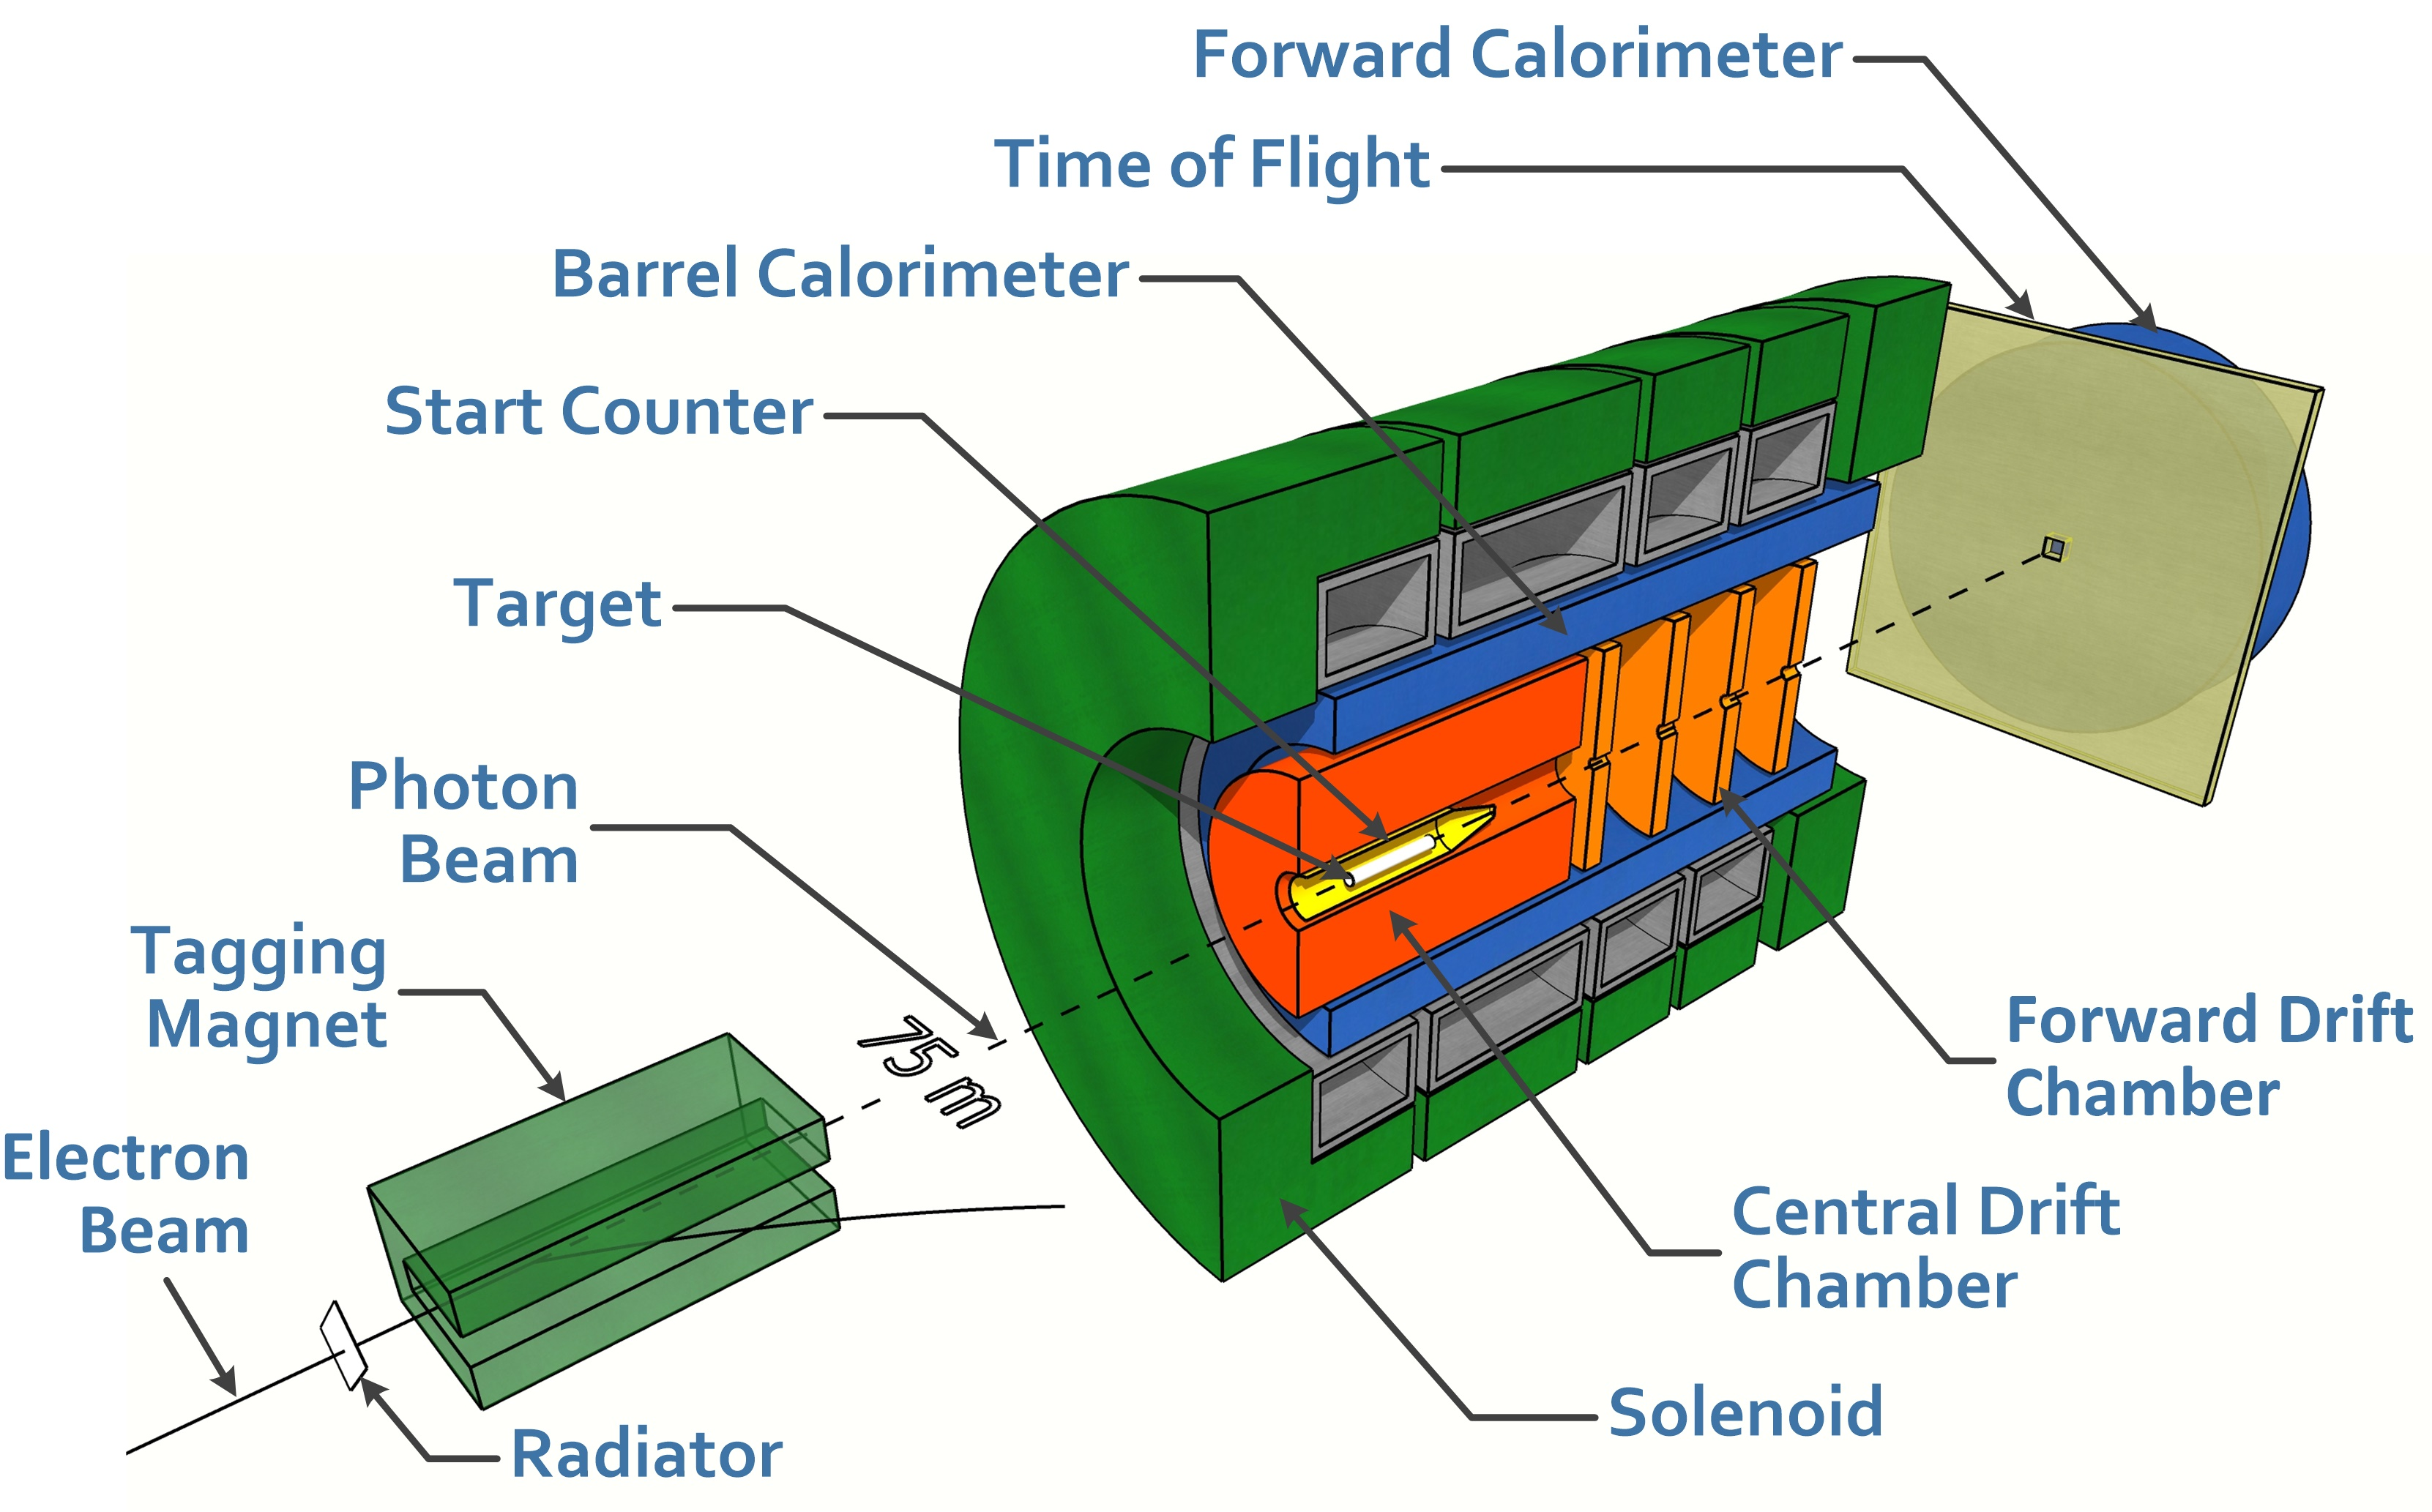
\includegraphics[width=0.75\textwidth]{figures/GlueX-graphic.jpg}
\caption[]{\label{fig:gluex_cut-away}(Color online)A cut-away drawing of the \GX{} detector in Hall D, not to scale.}
\end{figure}
The \emph{Glu}onic \emph{Ex}citation (\gx{}) experiment at the 
US Department of Energy's Thomas Jefferson National Accelerator Facility (JLab)\footnote{Thomas Jefferson National Accelerator Facility, 12000 Jefferson Ave., Newport News, VA 23606, https://www.jlab.org.} has been built to both search for and map out the spectrum of exotic hybrid mesons using a high-energy (9~GeV) linearly-polarized photon beam incident on a proton target\cite{gluex-ref}. The \gx{} detector and beamline are shown schematically in Figure~\ref{fig:gluex_cut-away}. The detector is nearly hermetic for both charged particles and photons arising from reactions in the crygenic target at the center of the detector, allowing for reconstruction of exclusive final states. A 2-T solenoidal magnet surrounds the drift-chamber based tracking. Two electromagnetic calorimeters cover the central and forward regions, and a scintillation detector downstream provides particle-identification capability through time-of-flight measurements. 


\subsection[The Hall-D complex]{The Hall-D complex \label{sec:gluexexperiment:complex}}
The \gx{} experiment is housed in the Hall-D complex at JLab (see Fig.\ref{fig:CEBAF-graphic}). This new facility starts with an extracted electron beam at the north end of the Continuous Electron Beam Accelerator Facility (CEBAF) \cite{Leemann:2001dg}; this electron beam has the highest-energy electrons at the lab, up to 12~GeV, due to an extra one-half pass of acceleration relative to three other experimental halls (A, B and C). The electron beam enters the Tagger Hall and produces linearly polarized photons through coherent bremsstrahlung on a 50~$\mu$m thick diamond crystal radiator.
The scattered electrons pass through a tagger magnet and are bent into tagging detectors. A high-resolution scintillating-fiber tagging array covers the 8 to 9~GeV energy range, and a tagger hodoscope covers photon energies both from 9~GeV to the endpoint, and from 8~GeV to 3~GeV. Those electrons not interacting in the diamond are directed into a 60 kW electron beam dump. The tagged photons pass through a tunnel to the Hall-D experimental hall. The distance from the radiator to the 5~mm diameter primary collimator, which removes off-axis incoherent photons, is 75 m. The front face of the collimator is instrumented with an active collimator to aid in beam tuning.  The beamline and tagging system are described below in Section\,\ref{sec:beamline}.

Downstream of the primary collimator is a thin beryllium radiator used by both the Triplet Polarimeter, which measures the linear polarization of the photons, and a Pair Spectrometer, which is used to measure the flux of the photons. More information on the production, tagging and monitoring of the photon beam can be found in Section~\ref{sec:beamline}. The photons then pass through a 30-cm-long liquid hydrogen target at the heart of the \gx{} detector. Photons which did not interact in the central target travel to the end of the experimental hall where they enter the photon beam dump.

\begin{figure}[tbp]\centering
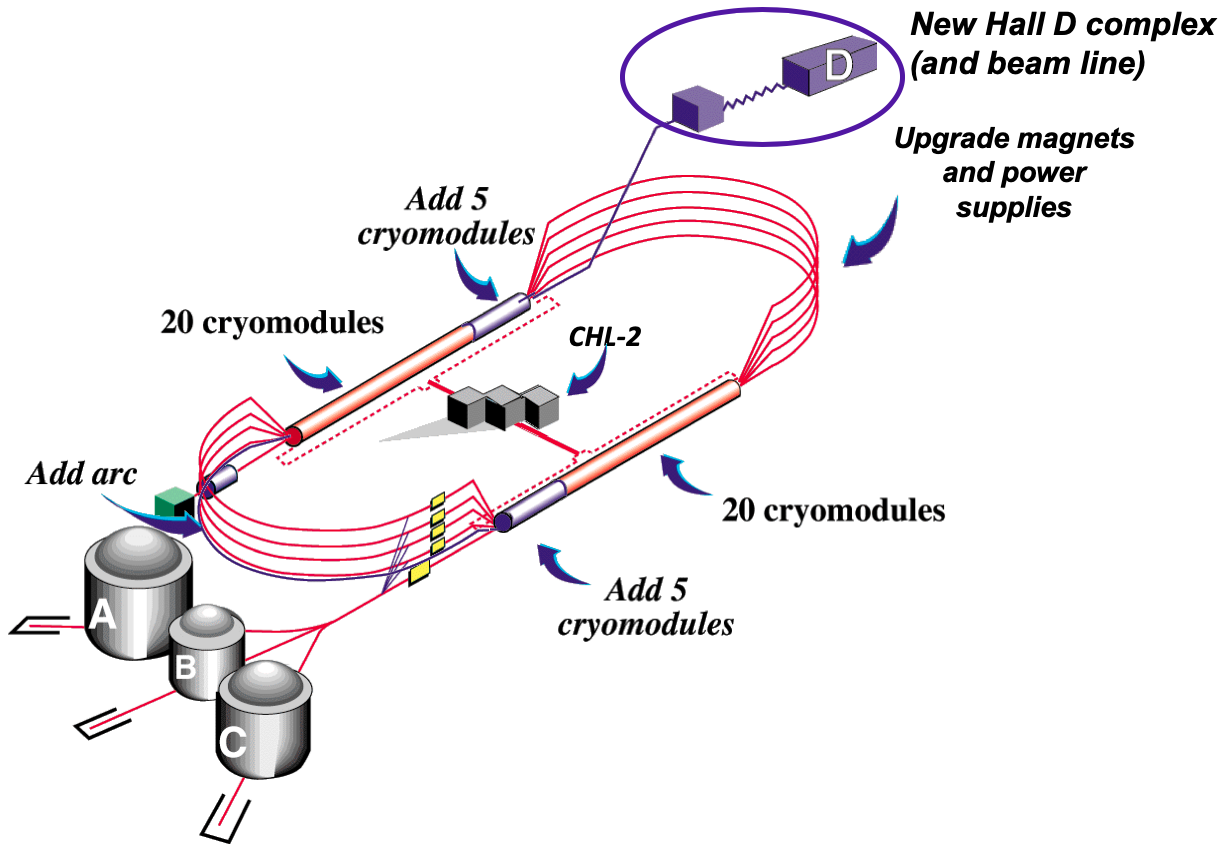
\includegraphics[width=0.75\textwidth]{figures/CEBAF-graphic.png}
\caption[]{\label{fig:CEBAF-graphic}(Color online) Schematic of the CEBAF accelerator showing the additions made during the 12-GeV project. The Hall D complex is located at the north-east end.}
\end{figure}

The \gx{} detector is based on a 4-m-long solenoidal magnet that is operated at a maximum field of 2~T. The layout of the detector is shown in Fig.~\ref{fig:layout_spectrometer}, while more information on the solenoid is provided in Section~\ref{sec:solenoid}. The liquid-hydrogen target is located 65~cm inside the upstream bore of the magnet. This target consists of a 2-cm-diameter, 29.25-cm-long volume of hydrogen, as described in Section~\ref{sec:target}. Surrounding the target is the Start Counter, which consists of 30 thin scintillator paddles that bend to a nose on the down-stream end of the hydrogen target. The Start Counter is the primary detector that identifies the radio-frequency (RF) bunch containing the incident electron associated with the tagged photon yielding the interaction. More information on the scintillator detector can be found in Section~\ref{sec:scintillators}. 

% ======================================================================================

\begin{figure*}[tbp]
\centering
  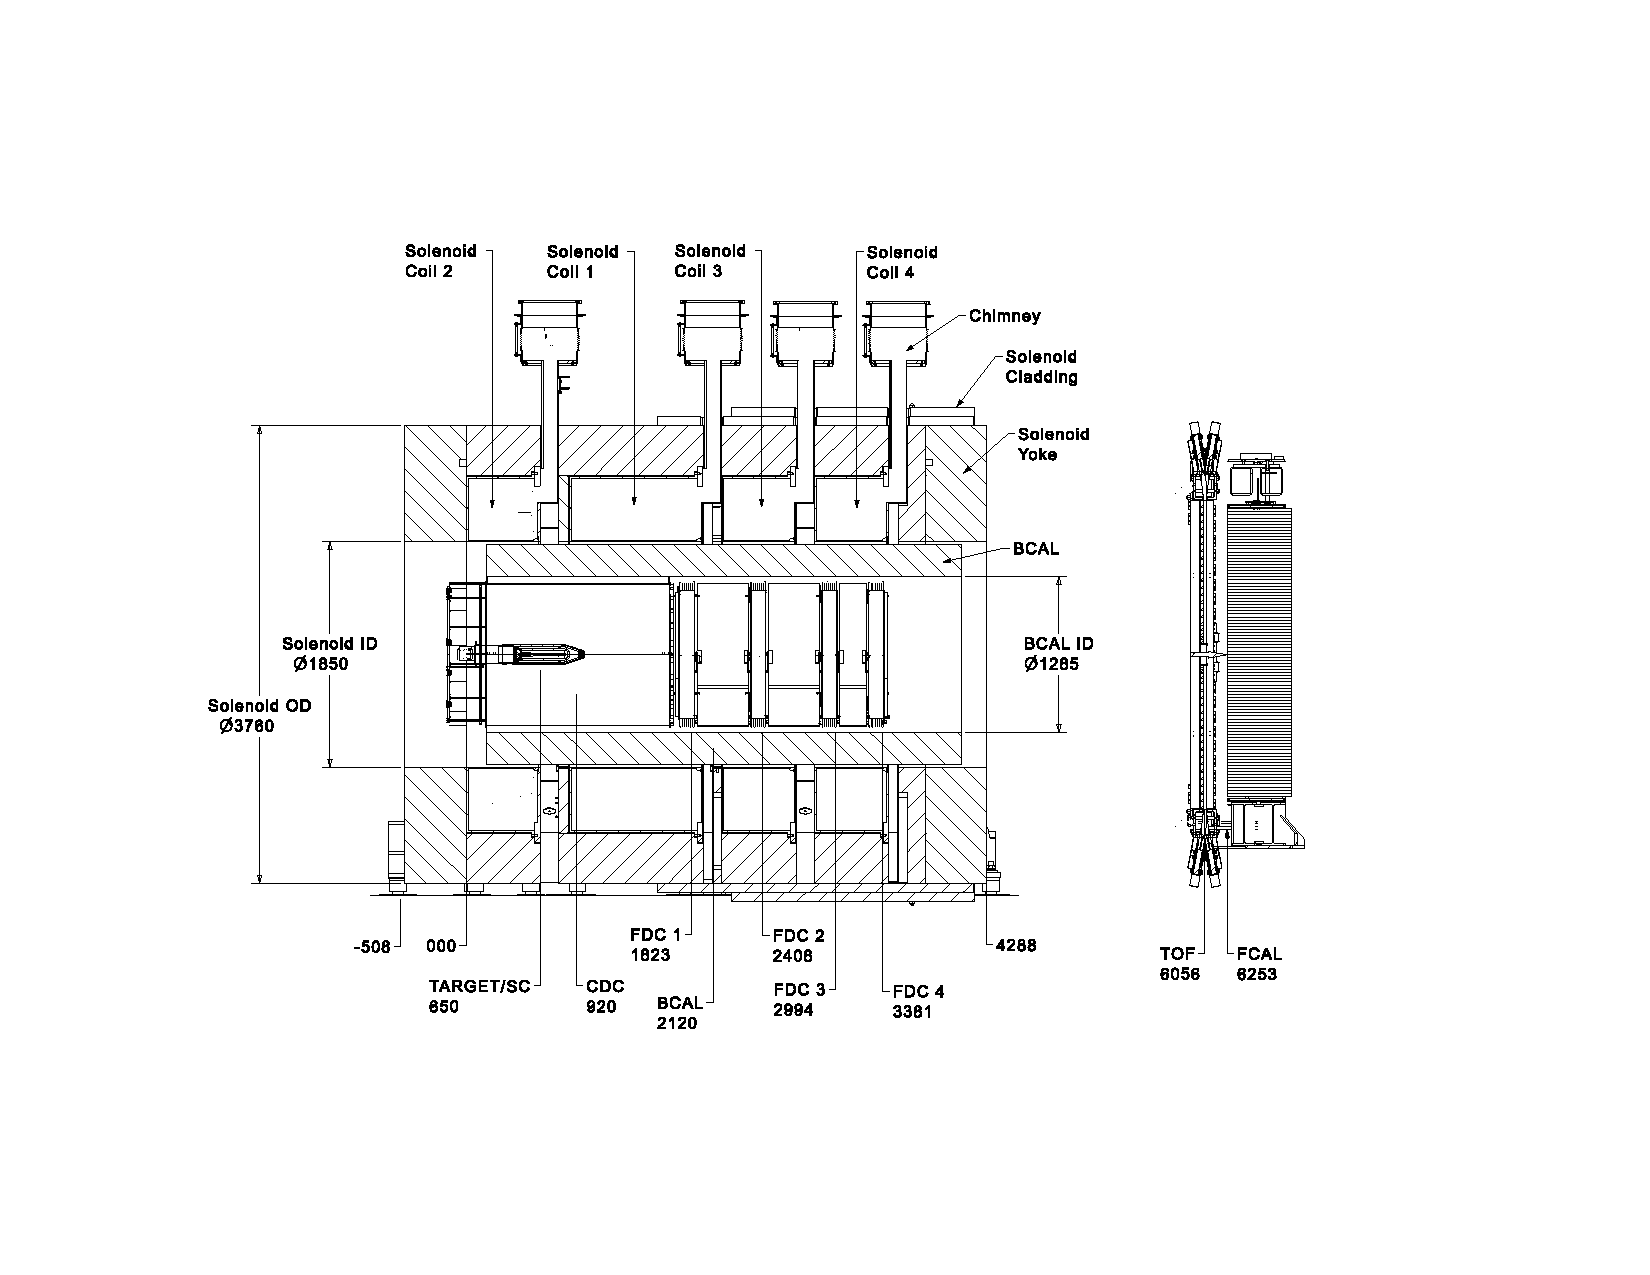
\includegraphics[angle=0,viewport=95 115 628 500,clip,width=1.0\linewidth]{figures/gluex_spectrometer_drawing_01_bw}%
  \caption[layout]{GlueX spectrometer layout. Dimensions are given in mm. The
    numbers show the Z-coordinates of the detectors' centers, or of
    the front face of the calorimeter modules in case of the FCAL.
    Glossary: 
              SC  - Start Counter (Section \ref{sec:st}), 
              CDC - Central Drift Chamber (Section \ref{sec:cdc}), 
              FDC - Forward Drift Chamber (Section \ref{sec:fdc}),
              BCAL - Barrel Calorimeter (Section \ref{sec:bcal}), 
              TOF -  Time-of-Flight hodoscope (Section \ref{sec:tof}), 
              FCAL - Forward Calorimeter (Section \ref{sec:fcal}).
%
%    \begin{tabular}{lll}
%       Name  & Detector & Section \\ \hline
%              SC  & Start Counter & \ref{sec:st} \\ 
%              CDC & Central Drift Chamber  & \ref{sec:cdc} \\ 
%              FDC & Forward Drift Chamber  & \ref{sec:fdc} \\ 
%              BCAL & Barrel Calorimeter    & \ref{sec:bcal} \\ 
%              TOF &  Time-of-Flight hodoscope & \ref{sec:tof} \\ 
%              FCAL & Forward Calorimeter    & \ref{sec:fcal} \\ 
%    \end{tabular}
    \label{fig:layout_spectrometer}
  }
\end{figure*}

% ======================================================================================


%\begin{figure}[htbp]\centering
%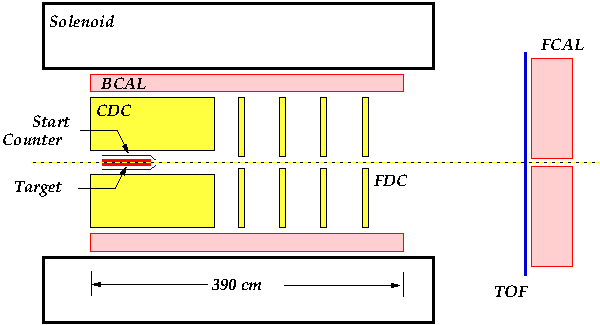
\includegraphics[width=0.7\textwidth]{figures/GlueX_Sketch.pdf}  
%\caption{\label{fig:gluexsketch} (Color online)         
%Sketch of GlueX detector.  The main systems of the detector are the Start %Counter \cite{Pooser:2019rhu}, the Central Drift Chamber (CDC) %\cite{VanHaarlem:2010yq} the Forward Drift Chamber (FDC) \cite{Pentchev2017281}, %a scintillator-based Time of Flight (TOF) wall and a lead-glass Forward %Calorimeter (FCAL) \cite{MORIYA201360}. The Barrel Calorimeter (BCAL) is %sandwiched between the drift chambers and the inner radius of the solenoid.}   
%\end{figure}

Starting at a radius of 10~cm from the beam line is the Central Drift Chamber, a cylindrical straw-tube detector. The active volume of the chamber extends from 48~cm upstream to 102~cm downstream of the target center, and from 10~cm to 56~cm in radius. The Central Drift Chamber consists of 28 layers of straw tubes in axial and two stereo orientations. Downstream of the central tracker is the Forward Drift Chamber, which consists of four packages, each containing 6 planar layers in alternating $u$-$y$-$v$ orientations. Both cathodes and anodes in the Forward Drift Chamber are read out, providing three-dimensional space point measurements. More details on the tracking system are provided in Sections~\ref{sec:tracking} and \ref{sec:trackingperformance}. 

Downstream of the magnet is the Time-of-Flight wall. This system consists of two layers of scintillator paddles in a crossed pattern, and, in conjunction with the Start Counter, is used to measure the flight time of charged particles. More information on the time-of-flight system is provided in Section~\ref{sec:scintillators}. 
Photons arising from interactions within in the \gx{} target are detected by two calorimeter systems. The Barrel Calorimeter, located inside the solenoid, consists of layers of scintillating fibers alternating with lead sheets. The Forward Calorimeter is downstream of the Time-of-Flight wall, and consists of $2800$ lead-glass blocks. More information on the the calorimeters can be found in Section~\ref{sec:calorimeters}.

\subsection[Experimental Requirements]{Experimental Requirements \label{sec:intro:requirements}}
In order to reconstruct exclusive final states, the \gx{} detector must be able to reconstruct both charged particles ($\pi^{\pm}$, $K^{\pm}$ and $p/\bar{p}$) and particles decaying into photons ($\pi^{\circ}$, $\eta$, $\omega$ and $\eta^{\prime}$). For this capability, the charged particles and photons must be reconstructed with good momentum and energy resolution. The experiment must also be able to reconstruct the energy of the incident photon (8 to 9~GeV) with high accuracy ($0.1$\%) and have knowledge of the linear polarization (maximum $\sim$40\%) of the photon beam to an absolute precision of 1\%. Finally, many interesting final states involve more than five particles. Thus, the \gx{} detector must also be nearly hermetic for both charged particles and photons, with an acceptance that is reasonably uniform, well understood, and accurately modeled in simulation.

In practice, the typical momentum resolution for charged particles is $1$--$3\%$, while for very-forward high-momentum particles the resolution is somewhat worse at around $8$-$9\%$. For most charged particles, the tracking system has nearly hermetic acceptance for polar angles in the lab from about $1^\circ-2^{\circ}$ to $150^{\circ}$. Due to the thickness of the hydrogen target, protons with momenta below about 250~MeV/c are not detected, and pions with momenta under 200~MeV/c can have spiraling trajectories in the detector, making reconstruction challenging. Energy loss ($dE/dx$) measured in the Central Drift Chamber can separate pions and protons up to about 800~MeV/c, while time-of-flight can separate forward-going pions and kaons up to about 2~GeV/c.

For photons produced from the decays of reaction products, the typical energy resolution is 5 to 6\%$/\sqrt{E_{\gamma}}$. Some variation exists in the Barrel Calorimeter resolution depending on the incident angle of the photon, but generally, photons above about 60~MeV can be detected. The interaction point along the beam direction is determined by comparing the information from the readouts on the upstream and downstream ends of the detector. The Forward Calorimeter can reconstruct photons whose energy is larger than 100~MeV, with uniform resolution across the face of the detector. There is a gap region between the calorimeters at around $11^{\circ}$, where energy can be lost due to leakage. Both photon detection efficiency and energy resolution are degraded in this region. 
 
\subsection{Data Requirements \label{sec:intro:data_requirements}}
To be able to carry out the physics analyses in small bins of energy and momentum transfer, the detector not only must have the ability to reconstruct exclusive final states but also collect sufficient statistics. While exact cross sections are not known, the cross sections of interest will be in the 10~nb range, with the largest cross sections of interest around 1~$\mu$b are expected. 

In operating the initial phase, the \GX{} experiment has run with a data acquisition system capable of collecting data using photon beams of a few $10^{7}~\gamma/$s in the coherent peak (8.4-9 GeV), with an expectation to run with about 2.5 times higher rates in the future. %\textcolor{blue}{(Do we want to mention the total photon flux above some cutoff energy? This may be better in the beamline section.)}
The data acquisition system ran routinely at 40\,kHz with raw event sizes of $15-20$ kilobytes, collecting about 600~megabytes of data per second. With trigger improvements, future running is expected at about 90 kHz and about 1~gigabyte per second. Details of the trigger and data acquisition are presented in Sections~\ref{sec:trig} and \ref{sec:daq}.

\subsection{Coordinate system \label{sec:intro:coordinates}}
For reference, we introduce here the overall experiment coordinate system, which is used in this document and throughout the analysis.
The experimental area is located 
off the northeast corner of the accelerator. The z-axis is defined along the nominal beamline increasing downstream (toward the east). The coordinate system 
is right-handed with the y-axis pointing vertically up and the x-axis pointing approximately north. 
The origin is located 50.8\,cm (20 inches) downstream of the upstream side of the upstream endplate of the solenoid, placing the nominal center of the target at (0,0,65\,cm).

\section[The coherent photon source and beamline]{The coherent photon source and beamline \label{sec:beamline}}
%{\color{red}General comment: As we haggle in the beamline group over the level of detail required for this section, it is worth bearing in mind that a longer-form paper dedicated to the beamline is also on our to-do list.  Material and detail felt to be excessive for this document can spill over into that paper}

\begin{table}[tbp]
\begin{center}
\caption
[Design properties of the electron beam]
{Electron beam parameters. 
The emittance, energy spread and       
related parameters are estimates
based on a model of the transport line from
the accelerator to the Hall D radiator.
The dimensions of the beam spot at the position of 
the radiator are directly measured, and vary around the
stated values by $\pm 30\%$
depending on beam conditions. 
Values for image size at collimator,
obtained by projection of the electron beam
spot convergence forward to the position of
the primary photon collimator, have relative
uncertainties of 50\%.
\label{tab:elecprop}}  
\begin{tabular}{|l|c|}
\hline\hline
parameter & design results \\
\hline
energy & 12~GeV \\ 
%electron polarization & available \\
energy spread, RMS & $2.2$~MeV \\
transverse $x$ emittance & 2.7~mm$\cdot\mu$rad \\
transverse $y$ emittance & 1.0~mm$\cdot\mu$rad \\
$x$ spot size at radiator, RMS & 1.1~mm \ \\
$y$ spot size at radiator, RMS & 0.7~mm \ \\
$x$ image size at collimator, RMS & 0.5~mm \\
$y$ image size at collimator, RMS & 0.5~mm \\
image offset from collimator axis, RMS & 0.2~mm \\
distance radiator to collimator & 75.3~m \\
\hline\hline
\end{tabular}
\end{center}
\end{table}

\subsection{CEBAF electron beam \label{sec:ebeam}}
CEBAF has a race track configuration with two parallel linear accelerators based on superconducting radio frequency (RF) technology \cite{Leemann:2001dg}. The machine operates at 1.497 GHz and delivers beam to Hall D at 249.5~MHz.\footnote{Hall D beam at 499 MHz is possible, but not the norm.} Precise timing signals for the accelerator beam bunches are available to the experiment and are used to determine the time that individual photon bunches pass through the target. The nominal properties for the CEBAF electron beam to the Tagger Hall are listed in Table\,\ref{tab:elecprop}.
\begin{figure}[t]
\begin{center}
%   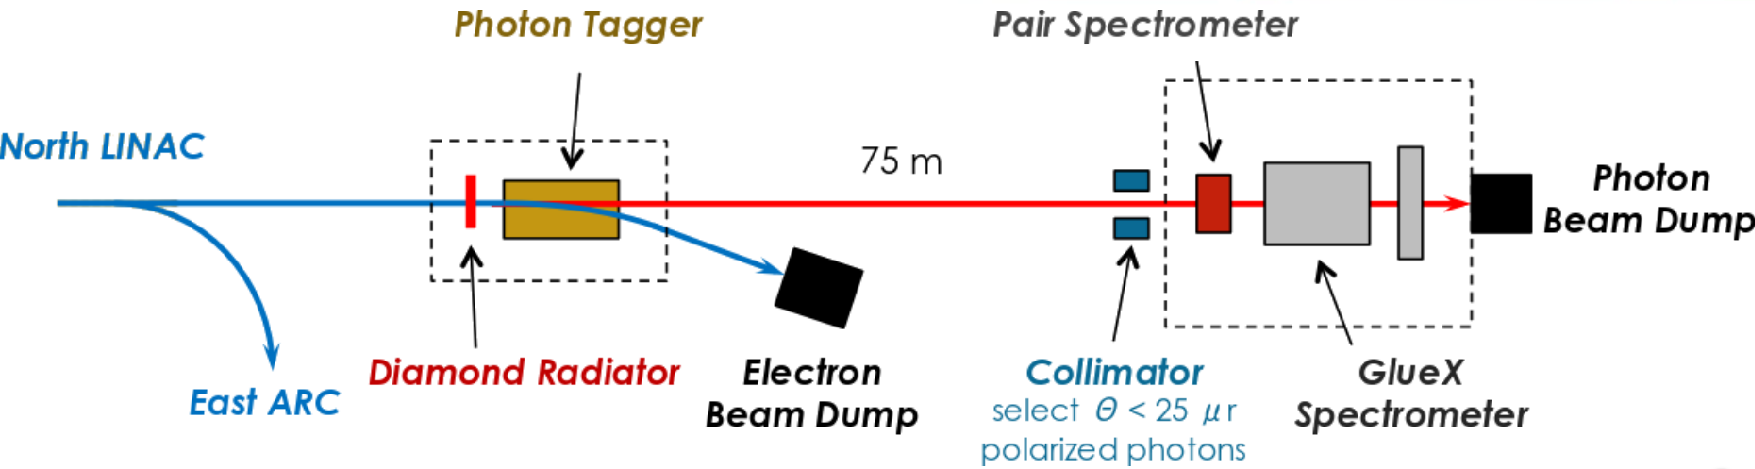
\includegraphics[clip=true,width=0.98\linewidth]{figures/gx_beamline_0}https://www.overleaf.com/6913428728kzgcdrhmtbjj
 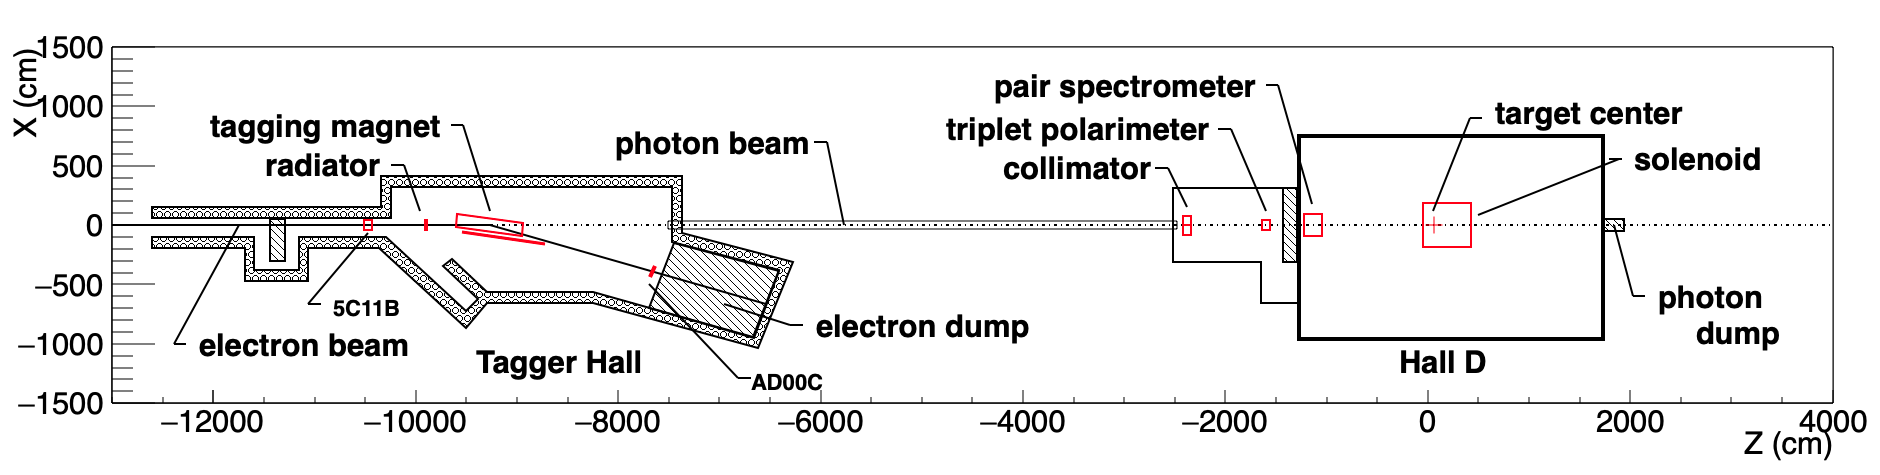
\includegraphics[clip=true,width=0.98\linewidth]{figures/Draw_beamline.png}
\end{center}
\caption{Schematic layout of the Hall-D complex, showing the Tagger Hall, Hall D, and
several of the key beamline devices.
Also indicated are the locations of the 5C11B and AD00C beam position monitors.
        }
\label{fig:beam:Draw_beamline} 
\end{figure}

\subsection{Hall-D photon beam \label{sec:gbeam}}
The Hall-D complex, described in Section \ref{sec:gluexexperiment:complex} and shown schematically in Fig.~\ref{fig:beam:Draw_beamline}, includes a dedicated Tagger Hall, an associated collimator cave, and Experimental Hall D itself. A linearly-polarized photon beam is created using the process of coherent bremsstrahlung \cite{timm1969,LIVINGSTON2009205} when the electron beam passes through an oriented diamond radiator at the upstream end of the Tagger Hall.
The electron beam position at the radiator is monitored and controlled using beam position monitors (5C11 and 5C11B) which are located at the end of the accelerator tunnel just upstream of the Tagger Hall (see Fig.\,\ref{fig:beam:Draw_beamline}.)
%The position of the beam on the collimator is initially set by adjusting small corrector magnets at this location.
The CEBAF electron beam is tuned to converge as it passes through the radiator, ideally
so that the electron beam forms a virtual focus at the collimator 
located 75\,m downstream of the radiator.
At the collimator, the virtual spot size of 0.5\,mm is small compared to the cm-scale size of the photon beam on the front face of the collimator,
such that a cut on photon position at the collimator is effectively a cut on photon emission angle at the radiator. 
The convergence properties of the electron beam are measured by scanning the beam profile with vertical and horizontal wires. The wire scanners are referred to as "harps."
Examples of the horizontal and vertical convergence of the electron beam envelope (undeflected by the tagger magnet)
measured using harp scans and projected downstream along the beamline are shown in Fig.\,\ref{fig:beam:convergence}.

\begin{figure}[tbp]
\begin{center}
 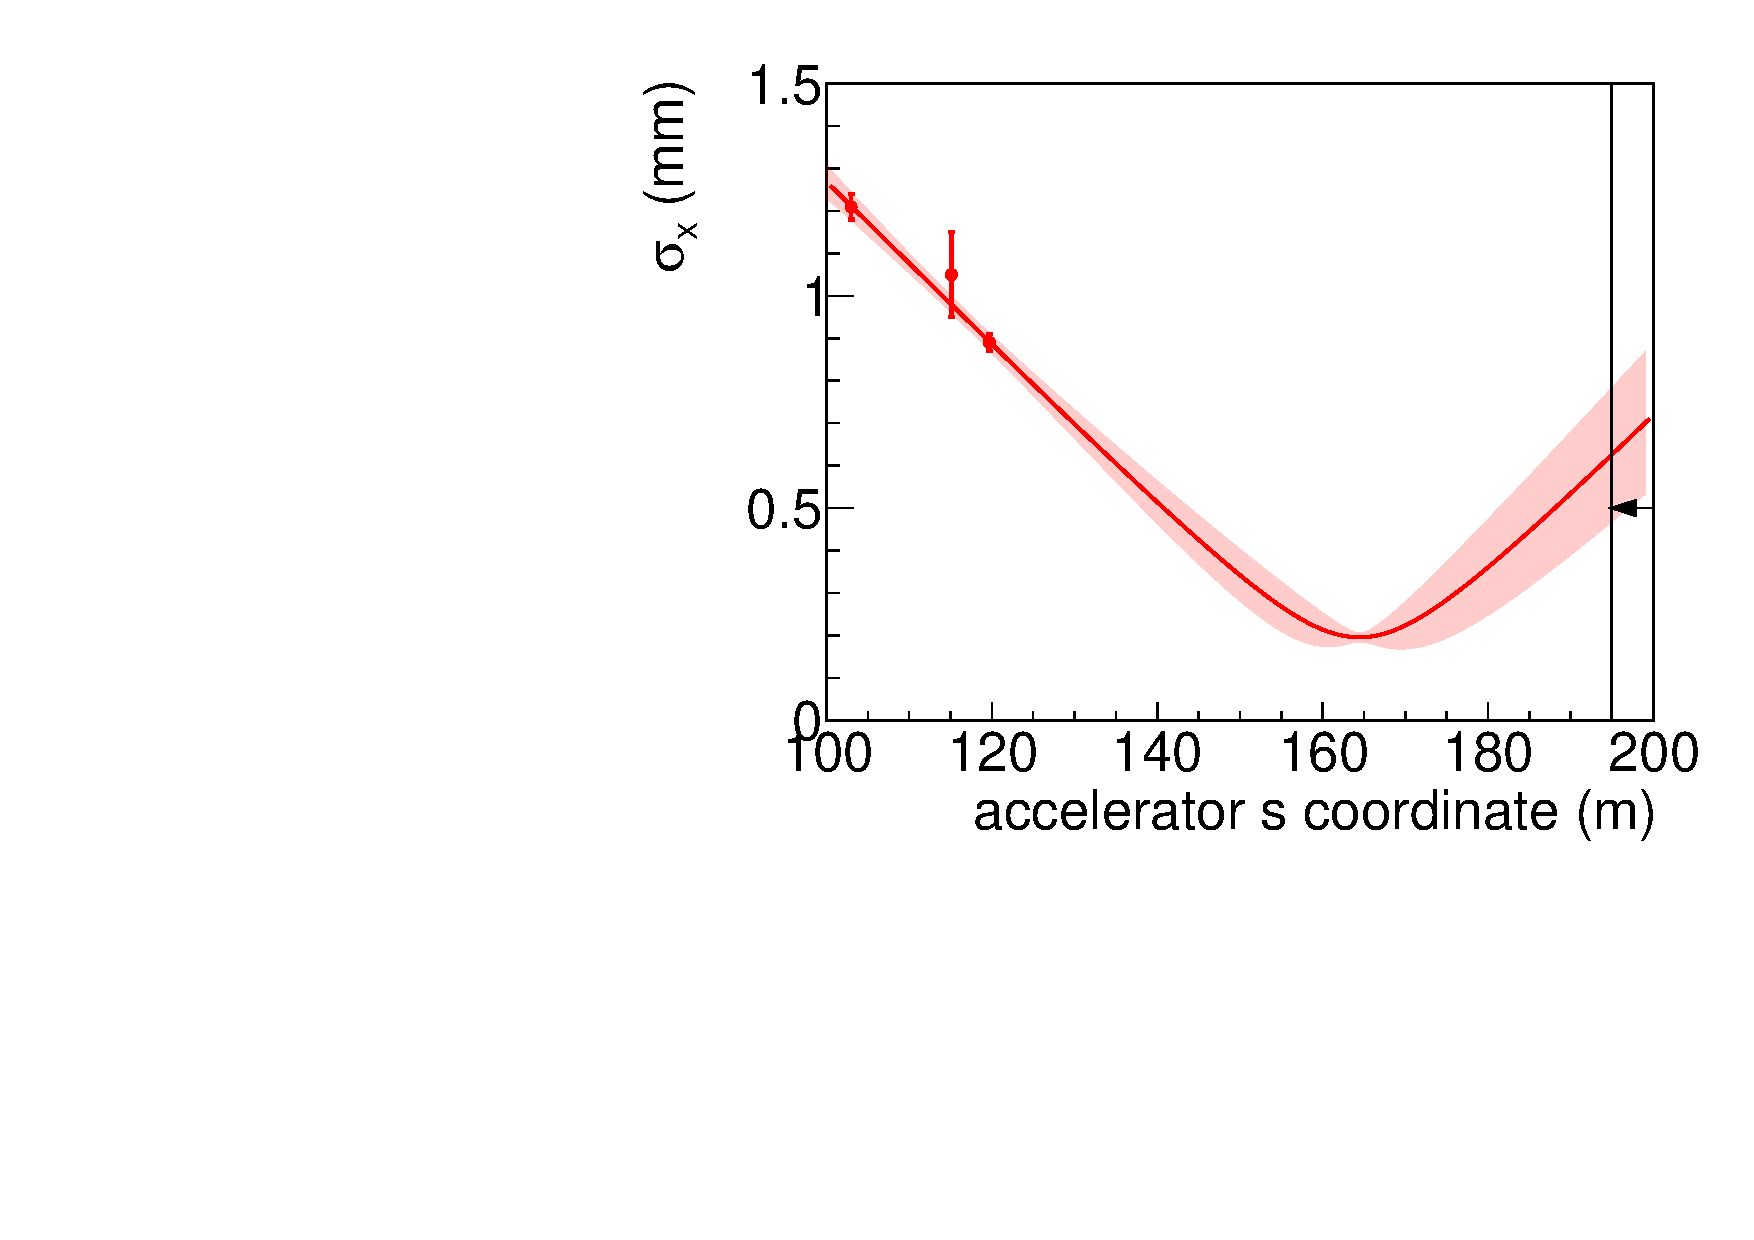
\includegraphics[clip=true,width=0.49\linewidth]{figures/harp-x-767755.pdf}
 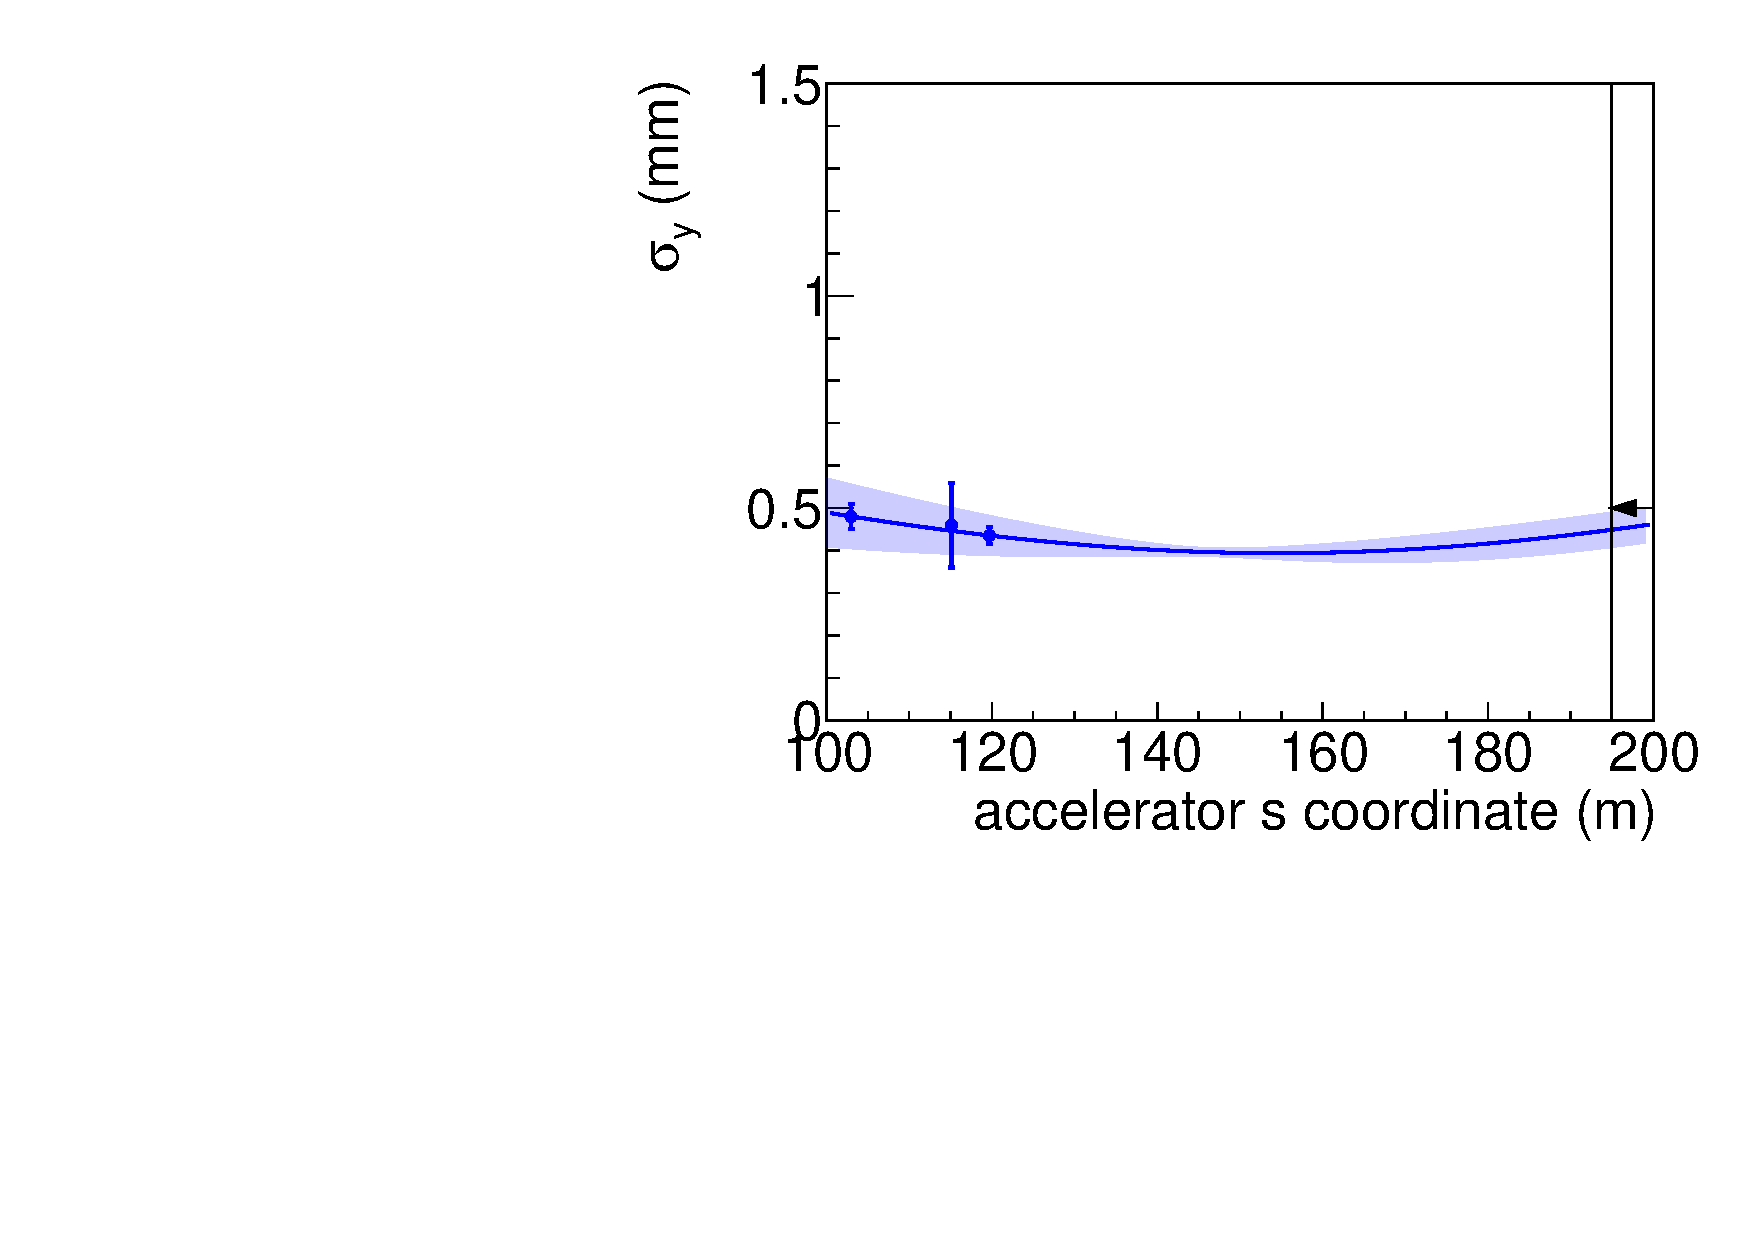
\includegraphics[clip=true,width=0.49\linewidth]{figures/harp-y-767755.pdf}
\end{center}
\caption{(Color online) Measurements of the root-mean-square width of the electron beam 
in horizontal (left)
and vertical (right) projections as a function of position along the beamline, based on
harp scans (data points) of the electron beam. The radiator position is just upstream
of the third data point. The primary collimator position is marked by the vertical line
indicated by the arrow. The curve downstream of the radiator is an extrapolation from
the measured data points, with extrapolation uncertainty indicated by the shaded regions.
        }
\label{fig:beam:convergence} 
\end{figure}

The photon beam position on the collimator is monitored using an active collimator positioned just upstream of the primary photon beam collimator
(described below in section \ref{sec:coll}). 
The position stability of the photon beam is maintained during normal
operation by a feedback system that locks the position of the electron
beam at the 5C11B beam position monitor and, consequently, the photon beam at the active collimator. The stability of the electron
beam current and position is monitored using an independent beam position monitor
(AD00C in Fig.\,\ref{fig:beam:Draw_beamline}) 
located immediately upstream of the electron dump.

%\begin{figure}[t]
%\begin{center}
%   %\includegraphics[viewport=1 1 790 %540,clip,angle=0,width=0.98\linewidth]{figs/mainmachine_beamline_dwg}
%\end{center}
%\caption{Schematics of the accelerator and the beam extraction system.
%        }
%\label{fig:beam:cebaf-dwg} 
%\end{figure}



The linearly-polarized photon beam is produced via a radiator placed in the electron beam just upstream of the
Tagger (section \ref{sec:tag}). A properly aligned 20--60\,$\mu$m thick diamond crystal
radiator produces
linearly polarized photons via coherent brems\-strah\-lung in enhancements \cite{timm1969,LIVINGSTON2009205},
that appear as peaks at certain energies in the brems\-strah\-lung intensity spectrum (Fig.\,\ref{fig:beam:gx3102_pi0etaAsym2016_fig0_beam}), superimposed upon the ordinary  continuum brems\-strah\-lung spectrum.
The energies of the coherent photon peaks and the degree of polarization in each of those peaks depend on the crystal orientation with respect to the incident electron beam.
Adjustment of the orientation of the diamond crystal with respect to the incoming
electron beam permits production of essentially any coherent photon peak energy up to that of the energy of the incident electron beam, as well as the
degree or direction of linear polarization.
A choice of 9 GeV for the primary peak energy, corresponding to 40\% peak linear polarization,
was found to be optimum for the \GX{} experiment with a 12-GeV incident electron beam.

\begin{figure}[tbp]
\begin{center}
 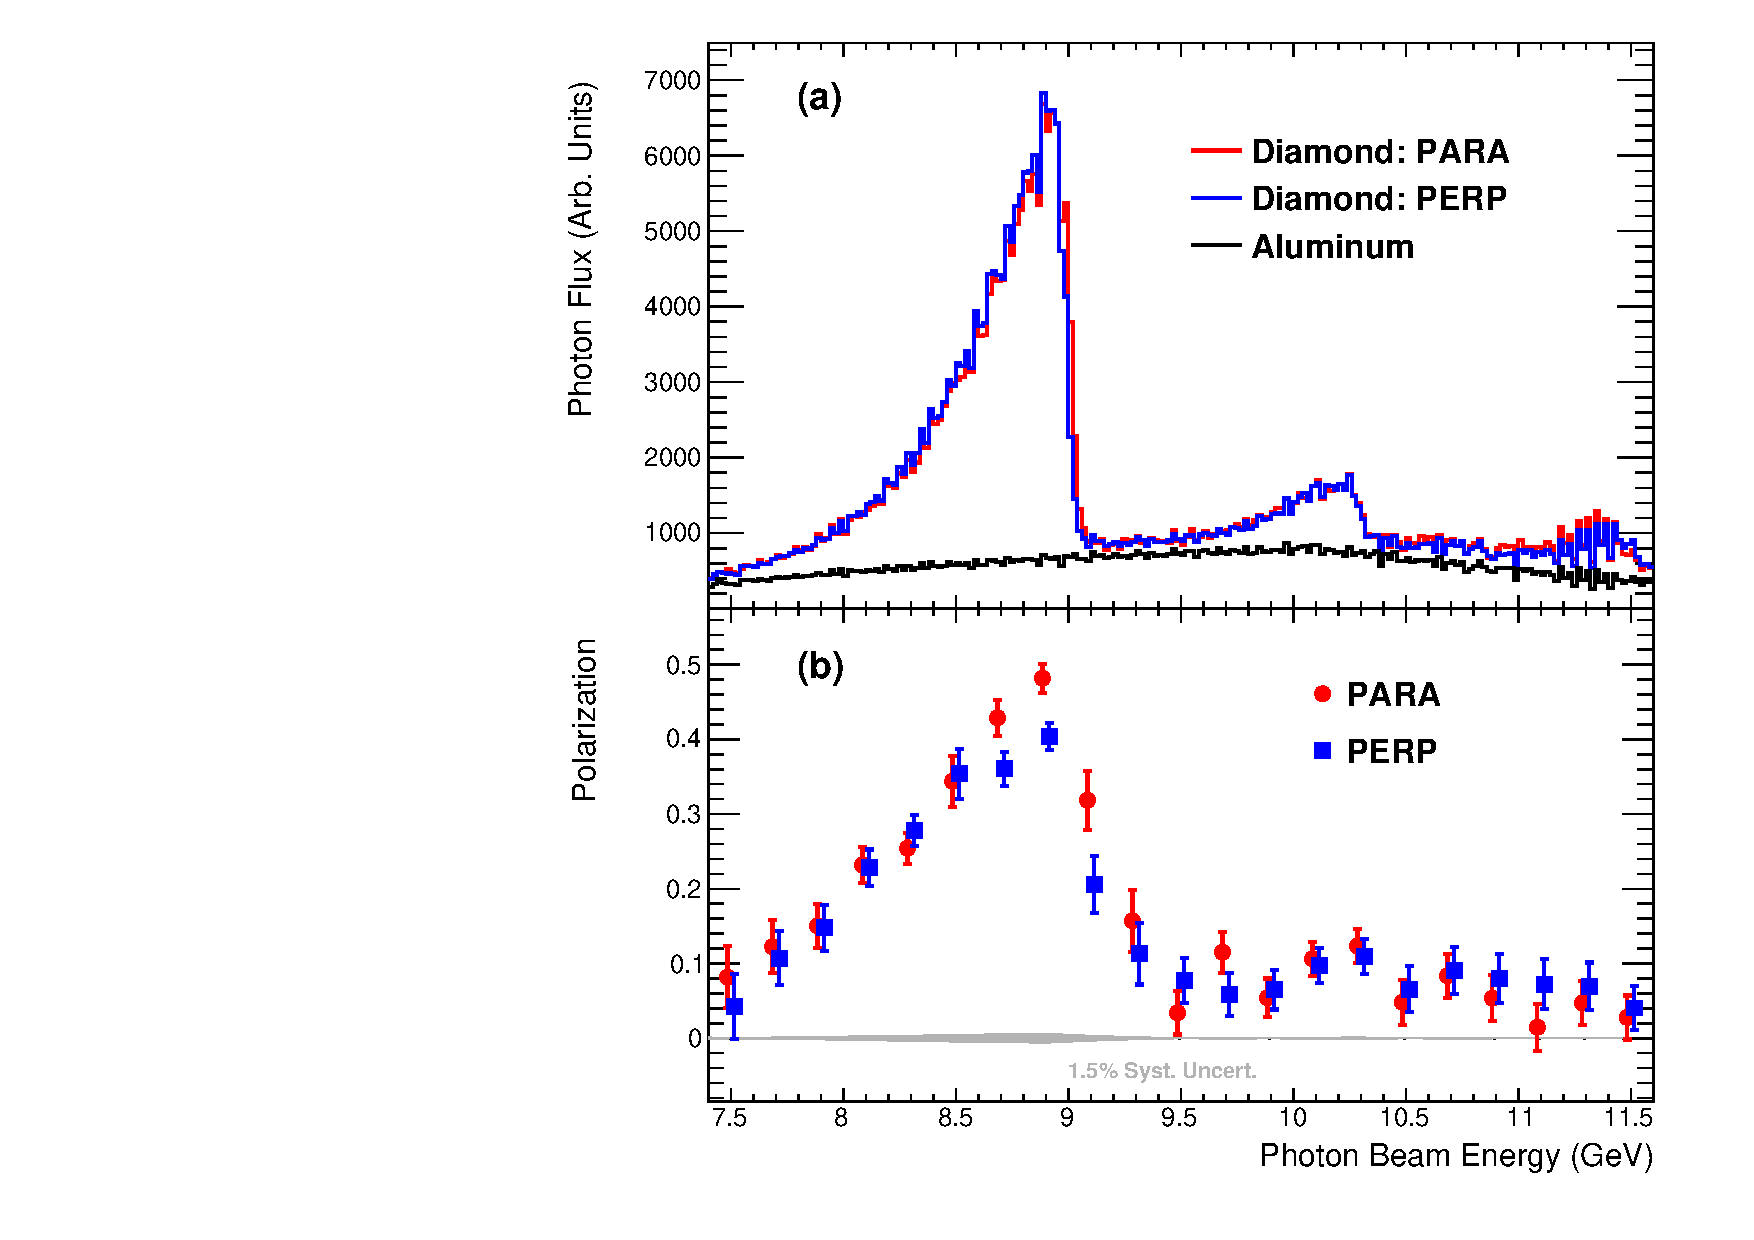
\includegraphics[clip=true,width=0.5\linewidth]{figures/gx3102_pi0etaAsym2016_fig0_beam.pdf}
\end{center}
\caption{(color online) (a) Photon beam intensity versus energy as measured by the Pair Spectrometer
(not corrected for instrumental acceptance).  (b) Photon beam polarization as a function of beam energy,
as measured by the Triplet Polarimeter, with data points offset horizontally by $\pm0.015$~GeV for clarity.
The labels PARA and PERP refer to orientations of the diamond radiator that result in polarization
planes that are parallel and perpendicular to the horizontal, respectively.
        }
\label{fig:beam:gx3102_pi0etaAsym2016_fig0_beam} 
\end{figure}

The degree of polarization for a coherent bremsstrahlung beam is greatest for photons emitted at small
angles with respect to the incident electron direction. Collimation of the photon beam to a fraction
of the characteristic brems\-strah\-lung angle exploits this correlation to significantly enhance
the average polarization of the beam. 
In the nominal \GX{} beamline configuration, a 5.0-mm-diameter collimator
\footnote{A 3.4\,mm collimator is also available, and has been used for some physics production runs
with the thinnest (20 $\mu m$) diamond.}
positioned 75\,m downstream of the radiator is used, corresponding to a cut at approximately
1/2 $m/E$ in characteristic angle, where $m$ is the electron rest mass and
$E$ is the energy of the incident electron. 
The photon beam energy spectrum and photon flux after collimation are measured
by the Pair Spectrometer (section \ref{sec:ps}), located downstream of the collimator in Hall D. 

An example of the measured photon spectrum and degree of polarization with a 12-GeV electron beam is
shown in Fig.\,\ref{fig:beam:gx3102_pi0etaAsym2016_fig0_beam}. The spectrum labeled ``Aluminum" in 
Fig.\,\ref{fig:beam:gx3102_pi0etaAsym2016_fig0_beam}(a) is shown to indicate the shape of the 
Pair Spectrometer acceptance folded with the spectrum of ordinary (incoherent) brems\-strah\-lung,
normalized to the approximate thickness of the diamond radiator in terms of radiation lengths.
The expected degree of linear polarization in the energy range of 8.4--9.0~GeV is $\sim$40\% after
collimation.  The photon beam polarization is directly measured by the triplet polarimeter (section \ref{sec:tpol})
located just upstream of the pair spectrometer. The stability of the beam polarization is independently
monitored via the observed azimuthal asymmetry in various photoproduction reactions, particularly that for $\rho$ photoproduction \cite{gx3076}.

Typical values for parameters and properties of the photon beam are given in Table\,\ref{tab:operates}.
In the sections that follow, we describe in more detail how the linearly-polarized photon beam
is produced, how the photon energy is determined using the tagging spectrometer, how the photon beam polarization
spectrum and flux are measured with the Pair Spectrometer and Triplet Polarimeter, and how the photon
flux is calibrated using the Total Absorption Counter.

\begin{table}[btp]
\begin{center}
\caption[Typical parameters for the \GX{} photon beam]{\label{tab:operates}
Typical parameters for the \GX{} photon beam,
consistent with the electron beam properties listed in Table \ref{tab:elecprop},
a diamond radiator of thickness 50~$\mu$m, and the standard primary collimator of diameter 5.0~mm
located at the nominal position. The electron beam current incident on the radiator is taken to  be $150$~nA.
The hadronic rates are calculated for the \GX{} 30~cm liquid hydrogen target.}
%\begin{tabular}{|l|c|c|c|c|}
%\hline\hline
%$E$ upper edge of the peak & 8~GeV & 9~GeV & 10~GeV & 11~GeV \\
%Peak FWHM & 1140~MeV & 900~MeV & 600~MeV & 240~MeV \\
%$N_{\gamma}$ in the peak & 185~MHz & 100~MHz & 45~MHz & 15~MHz \\
%polarization in the peak & 0.54 & 0.41 & 0.27 & 0.11 \\
%%\multicolumn{1}{c}{(F.W.H.M.)} & (1140 \Meunit) & (900 \Meunit) & (600 \Meunit) & (240 \Meunit) \\
%%(F.W.H.M.) & (1140) & (900 \Meunit) & (600 \Meunit) & (240 \Meunit) \\
%peak tagging efficiency & 0.55 & 0.50 & 0.45 & 0.29 \\
%%\multicolumn{1}{c}{(F.W.H.M.)} & (720 \Meunit) & (600 \Meunit) & (420 \Meunit) & (300 \Meunit) \\
%(F.W.H.M.) & (720 \Meunit) & (600 \Meunit) & (420 \Meunit) & (300 \Meunit) \\
%power on collimator & 5.3 W & 4.7 W & 4.2 W & 3.8 W \\
%power on target & 810 mW & 690 mW & 600 mW & 540 mW \\
%total hadronic rate & 385 kHz & 365 kHz & 350 kHz & 345 kHz \\
%tagged hadronic rate & 26 kHz & 14 kHz & 6.3 kHz & 2.1 kHz \\

% The number I entered came from the Bremstrahlung calculator, sometimes estimating averages from the plots
% Power and rates were taken from original table and reduced by a factor of 5.  ES 10/9/2019
\begin{tabular}{|l|r|}
\hline\hline
$E$ upper edge of the coherent peak & 9~GeV \\
Coherent peak effective range       & 8.4 - 9.0~GeV\\
Net tagger rate in the coherent peak range & 45~MHz  \\
$N_{\gamma}$ in the peak range after collimator & 24~MHz  \\
Maximum polarization in the peak, after collimator & 40\% \\
Mean polarization in the peak range, after collimator & 35\% \\
Power absorbed on collimator & 0.60~W \\
Power incident on target & 0.23~W \\
Total hadronic rate & 70 kHz \\
Hadronic rate in the peak range & 3.7 kHz \\
\hline\hline
\end{tabular}
\end{center}
\end{table}


\subsection{Goniometer and radiators \label{sec:radiators}}
For the linearly-polarized photon beam normally used in \GX{} production running, diamond radiators 
are used to produce a coherent bremsstrahlung beam. This requires precise alignment of the diamond
radiator, in order to produce a single dominant coherent peak\footnote{Defined as 0.6 GeV below the coherent edge (nominally 9 GeV). The position of the edge scales approximately with the primary incident electron beam energy.}  with the desired energy and polarization
by scattering the beam electrons from the crystal planes associated with a particular reciprocal lattice
vector.
A multi-axis goniometer, manufactured by Newport Corporation, precisely
adjusts the relative orientation of the
diamond radiator with respect to the incident electron beam horizontally, vertically and rotationally about the $X$, $Y$ and $Z$ axes, respectively.
The Hall-D goniometer holds several radiators, any of which may be moved into the beam for use at any time
according to the requirements of the experiment.

In addition to the diamond radiators, several aluminum radiators of thicknesses ranging from 1.5 to 40~$\mu$m are used to normalize the rate spectra measured in the Pair Spectrometer, correcting for its acceptance.
A separate rail for these amorphous radiators is 
positioned 615~mm downstream of the goniometer. 


\subsubsection{Diamond selection and quality control \label{sec:diamonds}}
The properties of diamond are uniquely suited for coherent brems\-strah\-lung radiators.
The small lattice constant and high Debye temperature of diamond result in an exceptionally high probability
for coherent scattering in the brems\-strah\-lung process \cite{Bilokon:1983}.
Also, the high coherent scattering probability is a consequence of the small atomic number of carbon (Z = 6). At the dominant crystal momentum (9.8 keV) corresponding to the leading (2,2,0) reciprocal lattice vector, the small atomic number results in minimal screening of the nuclear charge by inner shell electrons.
Diamond is the best known material in terms of its coherent radiation
fraction, and its unparalleled thermal conductivity and radiation hardness make it
well-suited for use in a high-intensity electron beam environment.

The position of the coherent edge in the photon beam intensity spectrum is a simple monotonic
function of the angle between the incident electron beam direction and the normal to the (2,2,0)
crystal plane. The 12-GeV-electron beam entering the radiator has a divergence less than
10 $\mu$rad, corresponding to a broadening of the coherent edge in
Fig.\,\ref{fig:beam:gx3102_pi0etaAsym2016_fig0_beam} by just 7~MeV. However, if the 
incident electron beam had 
to travel through 100~$\mu$m of diamond material prior to radiating, the
resulting electron beam emittance would
increase by a factor of 10 due to multiple Coulomb scattering, resulting in a proportional increase
in the width of the coherent edge. Such broadening of the coherent peak diminishes both the degree of polarization in the coherent peak as well as the collimation efficiency in the forward direction.
Hence, diamond radiators for \GX{} must be significantly
thinner than 100 microns. 

The cross-sectional area of a diamond target must also be large enough to completely contain the electron beam so that the beam does not overlap with the material of the target holder. Translated to the beam spot dimensions from Table\,\ref{tab:elecprop}, \gx{}
requires a target with transverse size 5~mm or greater. Uniform single-crystal diamonds of
this size are now available as slices cut from natural gems, HPHT (high-pressure, 
high-temperature) synthetics, and CVD (chemical vapor deposition) single crystals. Natural gems are ruled out due to cost. HPHT crystals had been thought
to be far superior to CVD single crystals in terms of their diffraction widths, but our
experience did not bear this out. \GX{} measurements of the
x-ray rocking curves of CVD crystals obtained from the commercial vendor Element Six\footnote{Element Six, https://www.e6.com/en.} routinely
showed widths that were within a factor 2 of the theoretical Darwin width,
similar to the results we found for the best HPHT diamonds that were available to us
\cite{YANG2010719,YANG2012}.

\begin{figure}[tbp]
\begin{center}
 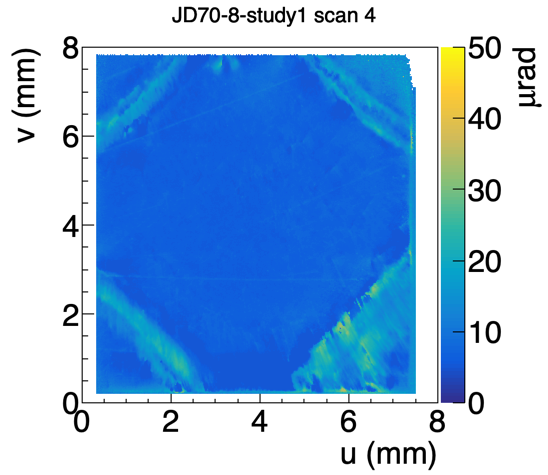
\includegraphics[clip=true,width=0.7\linewidth]{figures/JD70-8-study1_4_sigma.png}
\end{center}
\caption{(color online) Rocking curve RMS width topograph taken of the (2,2,0) reflection
from a CVD diamond crystal using 15~keV X-rays at the C-line at CHESS.
The bright diagonal lines in the corners
indicate regions of increased local strain, coinciding with growth boundaries radiating
outward from the seed crystal used in the CVD growth process. 
        }
\label{fig:diamond_rocking_curve_rms} 
\end{figure}

Fig.~\ref{fig:diamond_rocking_curve_rms} shows a rocking curve topograph of a diamond
radiator taken with 15~keV x-rays at the 
Cornell High Energy Synchrotron Source (CHESS). The instrumental
resolution of this measurement is of the same order as the Darwin width for this
diffraction peak, approximately 5 $\mu$rad. During operation, the electron beam spot would
be confined to the relatively uniform central region. Any region in
this figure with a rocking curve root-mean-square width of 20~$\mu$rad or less is indistinguishable
from a perfect crystal for the purposes of \GX{}.
Regardless of whether or not better HPHT diamonds exist, these Element Six CVD diamonds have sufficiently narrow  diffraction widths for our application.  This, coupled with their lower cost relative to HPHT material, made
them the obvious choice for the Hall-D photon source.

The diamond radiator fabrication procedure began with procurement of the raw
material in the form of $7\times 7\times 1.2$~mm$^3$ CVD single-crystal plates from the
vendor. After x-ray rocking curve scans of the raw material were taken to verify crystal
quality, the acceptable diamonds were shipped to a second vendor, Delaware Diamond Knives (DDK). At DDK, the
1.2-mm-thick samples were sliced into three samples of 250 $\mu$m thickness each, then
each one was polished on both sides down to a final thickness close to 50 $\mu$m. The
samples, now of dimensions $7\times 7\times 0.05$~mm$^3$ were fixed to a small aluminum
mounting tab using a tiny dot of conductive epoxy placed in one corner.
These crystals were then returned to the synchrotron light source
for final x-ray rocking curve measurements prior to final
approval for use in the \GX{} photon source.

The useful lifetime of a diamond radiator in the \GX{} beamline is limited by the 
degradation in the sharpness of the coherent edge due to accumulation of radiation damage.
Experience during the early phase of \GX{} running showed that after exposure to
about 0.5 C of integrated electron beam charge, the width of the coherent edge 
increased enough that the entire coherent peak was no longer contained within the energy
window of the tagger microscope. When a crystal reached this degree of degradation, the
radiator was regarded as no longer usable, and a new crystal was installed.

During Phase 1 of \GX{}, radiator crystals were replaced three times due
to degradation, twice with 50~$\mu$m radiators and once with a 20~$\mu$m radiator. The 20-$\mu$m
diamond was introduced to test whether the reduced multiple Coulomb scattering 
might result in an
observable increase in peak polarization. This turned out not to be the case, for
two reasons. The first is that to take full advantage of the reduced multiple
scattering in the radiator for increased peak polarization, the collimator size 
must be reduced proportionally. A 3.4-mm-diameter collimator was available for
this purpose, but variability observed in the convergence properties of the electron
beam at the radiator overruled running with any collimator smaller than 5~mm,
even when a thinner radiator was in use.

The second reason is that any improvements
from reduced multiple scattering that came with the smaller radiator thickness
were more than offset by strong indications of radiation
damage that appeared not long after the 20~$\mu$m crystal was put into production.
The rapid appearance of radiation damage 
was partly due to the larger beam current (factor 2.5) that was needed to
produce the same photon flux as with a 50~$\mu$m crystal, but that factor alone
did not fully
explain what was seen. Subsequent x-ray measurements showed that a large buckling of
the 20~$\mu$m crystal had occurred in the region of the incident electron beam spot, 
evidently due to  local differential expansion of the diamond lattice arising from
radiation damage. Once the crystal buckled, the energy of the coherent
peak varied significantly across the electron beam spot, effectively broadening
the peak. Fortunately, the greater stiffness of a 50~$\mu$m crystal
appears to suppress this local buckling under similar conditions of radiation damage.

Based on these observations, 50~$\mu$m was selected as the
optimum thickness for \GX{} diamond radiators: thin enough to limit the effects
of multiple scattering and thick enough to suppress buckling from internal stress
induced by radiation damage. The effective useful lifetime of a 50~$\mu$m radiator
in the photon source is about 0.5 C integrated incident electron charge. 
This lifetime might be extended somewhat by the use of thermal annealing to partially remove the effects of radiation damage. 
This possibility will be explored when the pace of diamond replacement increases with the start of full-intensity running (\gx{} Phase 2) and the number of spent radiators starts to accumulate.

\begin{figure}[tbp]
\begin{center}
   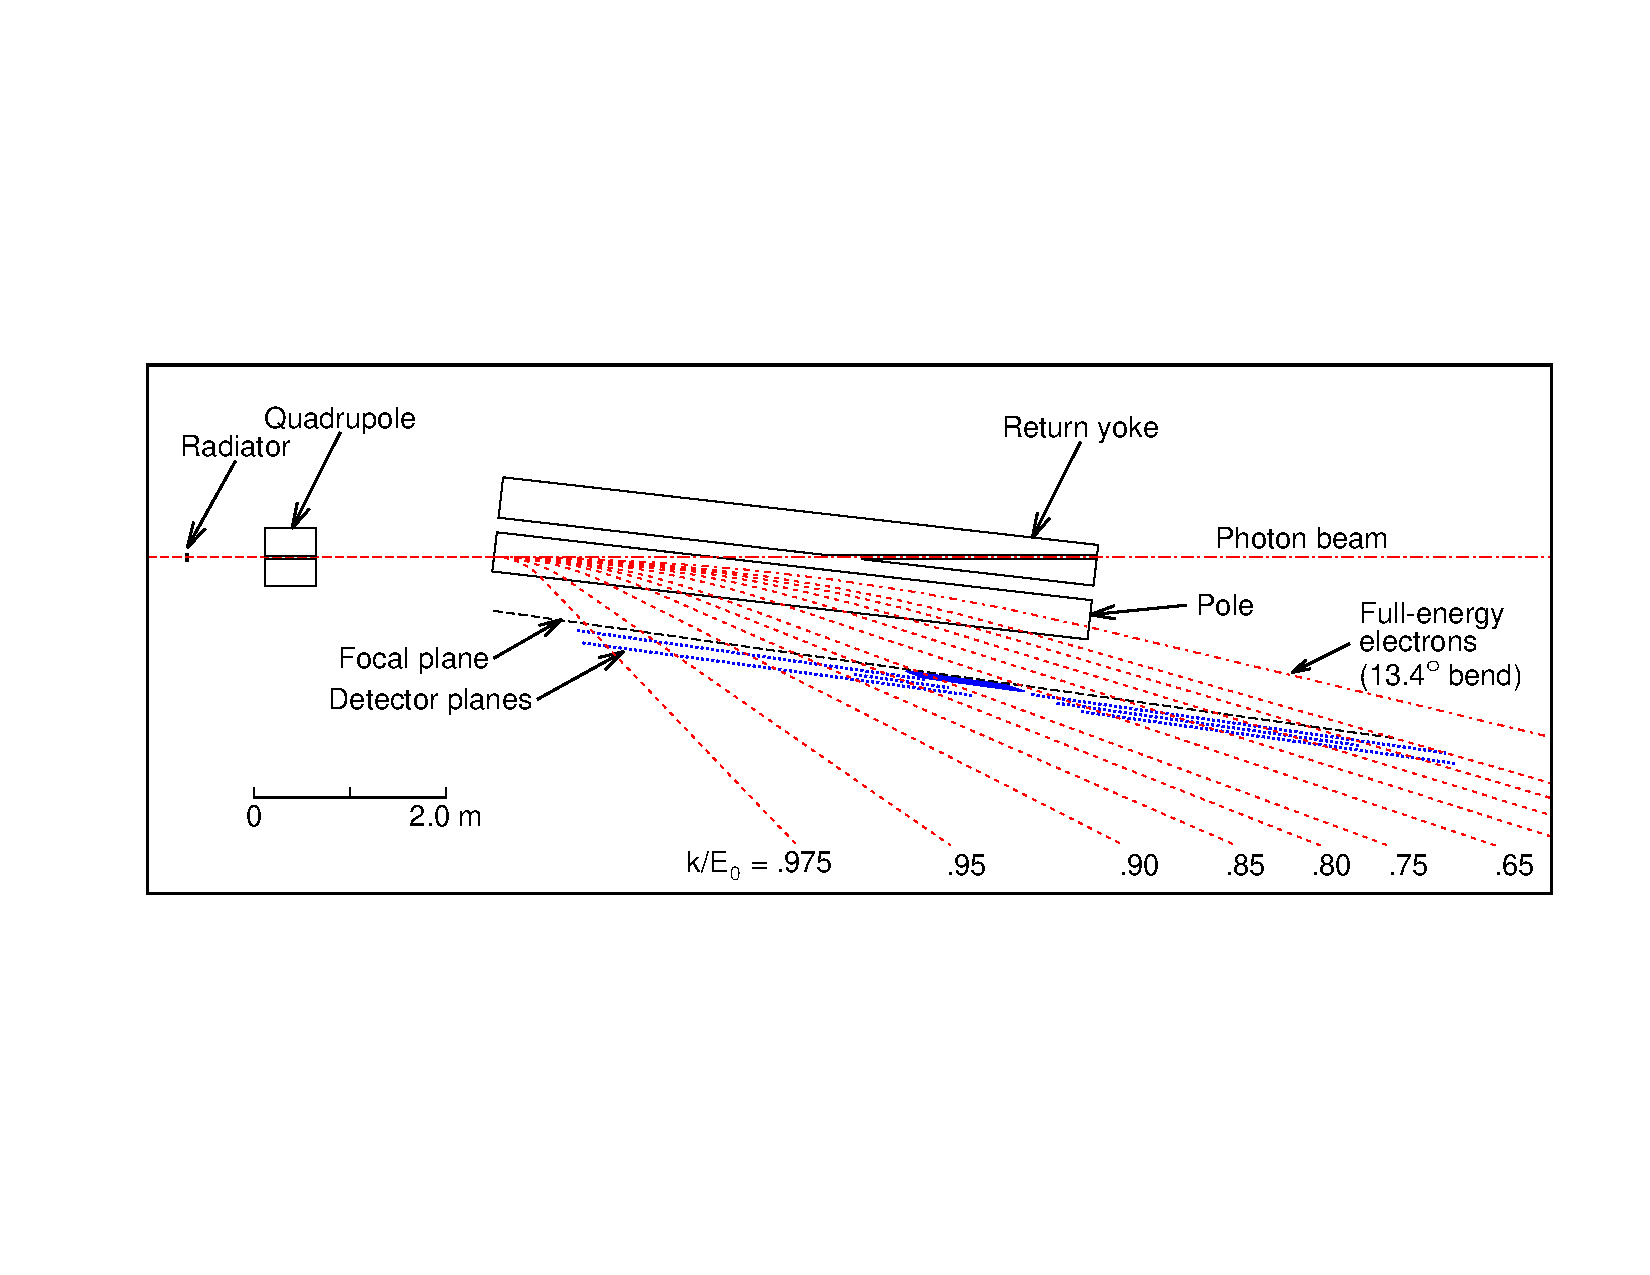
\includegraphics[width=0.95\linewidth,viewport=80 200 750 400]{figures/BEAM_taggerplot.pdf}
%   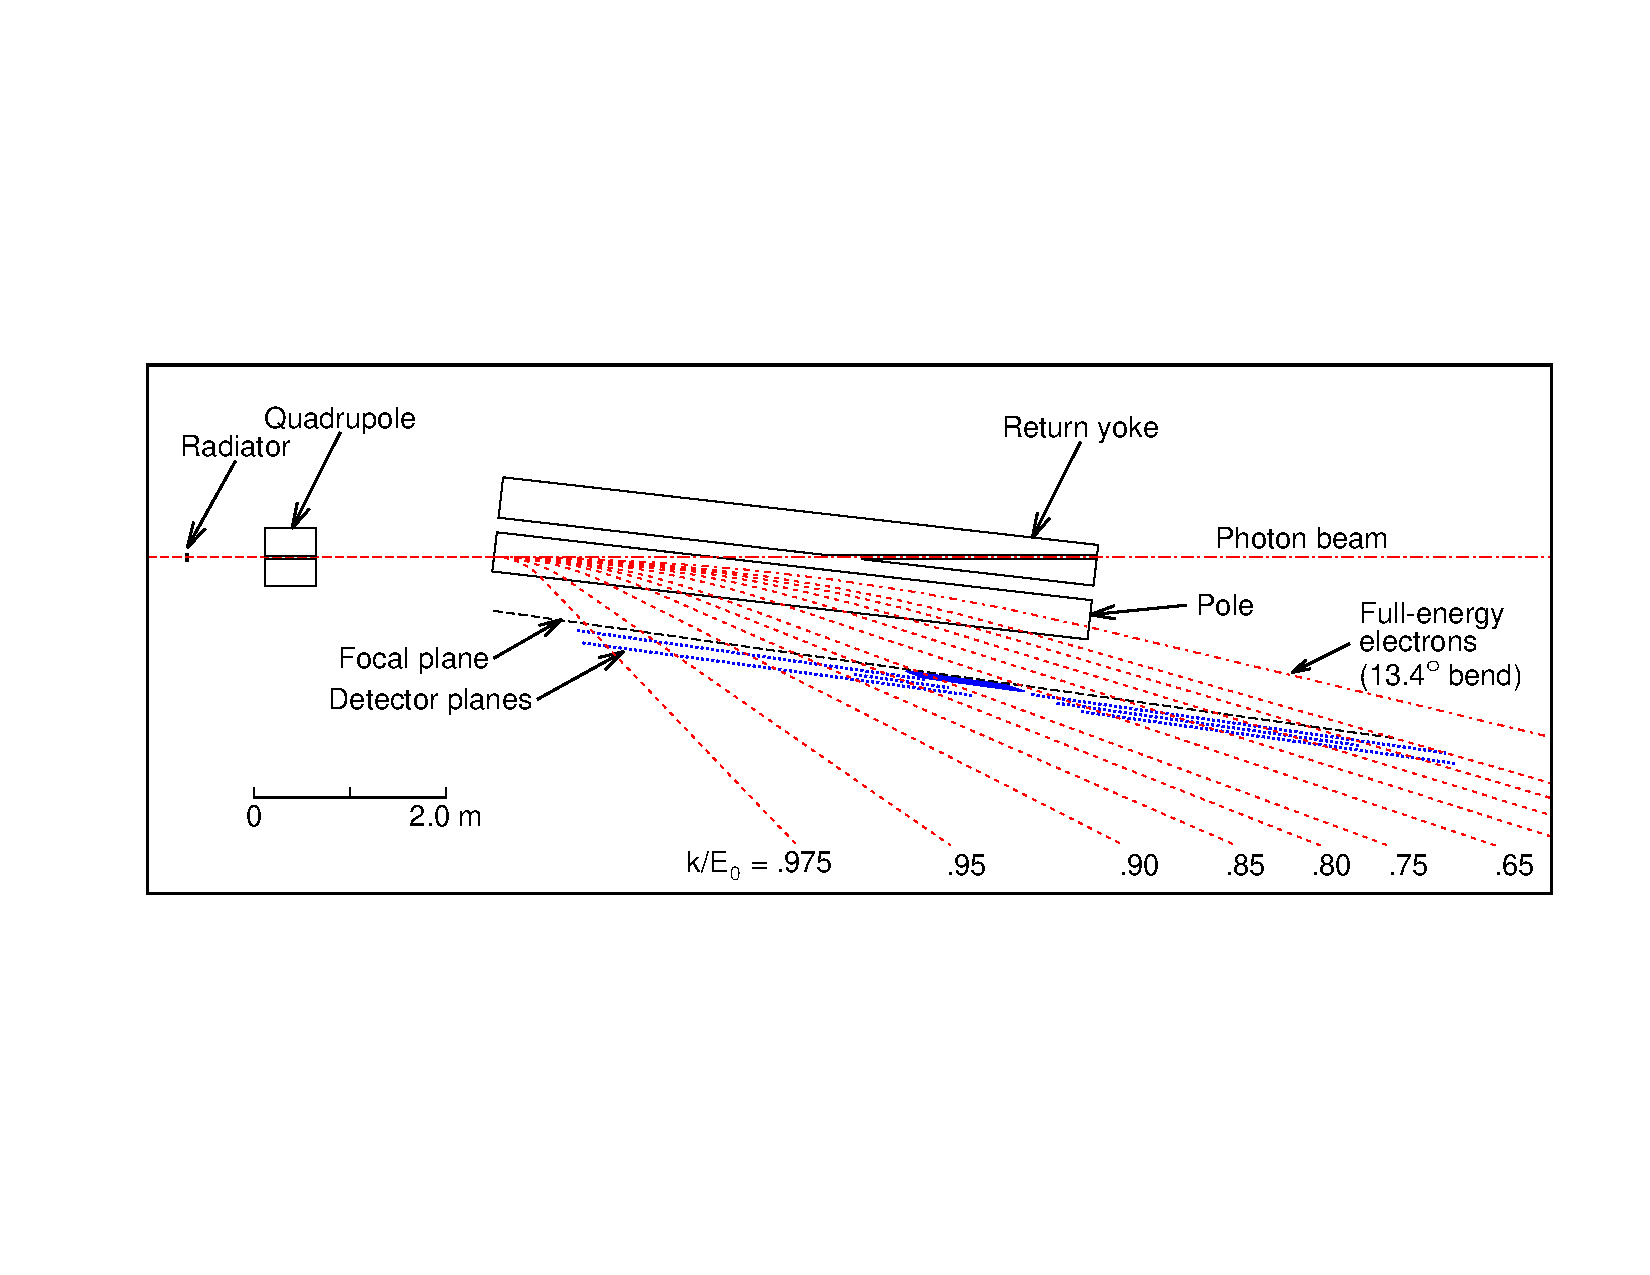
\includegraphics[width=0.95\linewidth,viewport=150 115 628 500]{figures/BEAM_taggerplot.pdf}
%      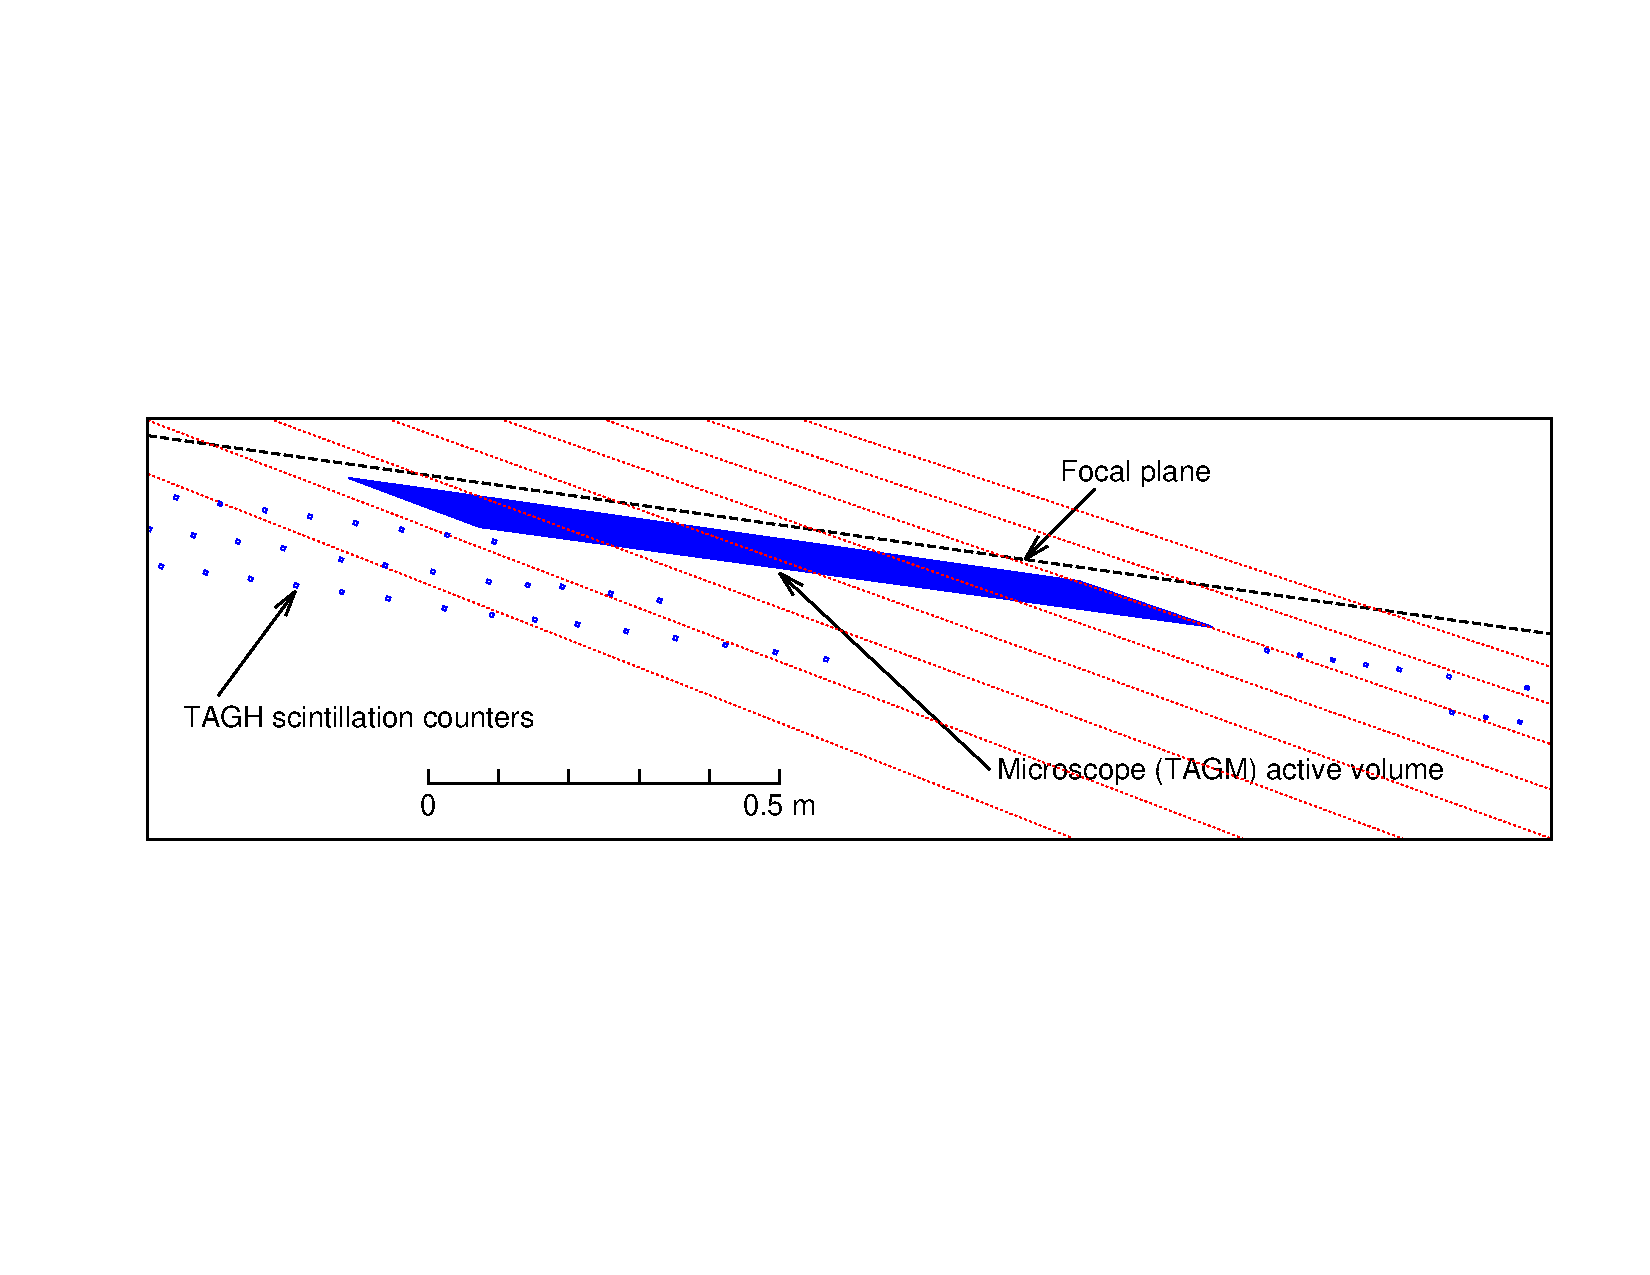
\includegraphics[width=0.95\linewidth]{figures/BEAM_taggerdetectors.pdf}
\caption{Schematic diagram of the tagging spectrometer, showing the paths of the electron
and photon beams. Dotted lines indicate post-radiation electron trajectories identified by
the energy the electron gave up to an associated radiated photon, as a fraction of the beam energy E$_0$.
The Tagger focal plane detector arrays TAGH and TAGM are described in the text.
       \label{fig:beam:BEAM_taggerplot}  }
\end{center}
\end{figure}

\subsection{Photon tagging system \label{sec:tag}}
After passing through the radiator, the combined photon and electron beams enter
the photon tagging spectrometer (Tagger). The full-energy electrons are swept out of
the beamline by a dipole magnet and redirected into a shielded beam dump. The
subset of beam electrons that radiated a significant fraction of their energy in
the radiator are deflected to larger angles by the dipole field. 
These post-brems\-strah\-lung electrons exit through a thin window
along the side of the magnet, and are detected in a highly segmented
array of scintillators called the Tagger Hodoscope, as shown in
Fig.\,\ref{fig:beam:BEAM_taggerplot}. The TAGH counters span
the full range in energy from 25\% to 97\% of the full electron beam energy. A high-energy-resolution device known as the Tagger Microscope (TAGM) covers the
energy range corresponding to the primary coherent peak, indicated by the denser
portion of the focal plane in Fig.\,\ref{fig:beam:BEAM_taggerplot}. 
The quadrupole magnet upstream of the Tagger dipole provides a weak vertical focus, optimizing the efficiency of the Tagger Microscope for tagging collimated photons.
A 0.8~Tm permanent dipole magnet is installed downstream of the Tagger magnet on the photon beam line, in order to prevent the electron beam from reaching Hall D should the Tagger magnet trip.

Both the TAGM and TAGH devices are used to determine the energy of individual
photons in the photon beam via coincidence, using
the relation $E_{\gamma} = E_{0} - E_{e}$, where $E_{0}$ is the primary electron
beam energy before interaction with the radiator, and $E_{e}$ is the
energy of the post-brems\-strah\-lung electron determined by its detected position at the
focal plane. Multiple radiative interactions in a 50 $\mu$m diamond radiator
($3\times 10^{-4}$ radiation lengths) produce uncertainties in
$E_{\gamma}$ of the same order as the intrinsic energy spread of the incident
electron beam.

\subsubsection{Tagger magnet \label{sec:tagMagnet}}
The Hall-D Tagger magnet deflects electrons in the horizontal plane, allowing the
brems\-strah\-lung-produced photons to continue to the experimental hall while
bending the electrons that produced them into the focal plane detectors.
Electrons that lose little or no energy in the
radiator are deflected by 13.4$^\circ$ into the electron beam dump.

The Hall-D Tagger magnet is an Elbek-type room temperature dipole magnet, similar
to the JLab Hall-B tagger magnet \cite{BORGGREEN19631, Sober2000263}. 
The magnet is 1.13~m wide, 1.41~m high and 6.3~m long, weighing 80~metric tons,
with a normal operating field of 1.5~T for a  12-GeV incident electron beam, 
a maximum field of 1.75 T, and a pole gap of 30 mm. 
The magnet
design was optimized using the detailed magnetic field calculation  provided by the
TOSCA simulation package and ray tracing of electron beam trajectories~\cite{DIPOLE_YANG,DIPOLE_SOMOV}.

The \gx{} experiment requirements mandate that the scattered
electron beam be measured with an accuracy of 12~MeV (0.1\% of the incident electron
energy). This requires that the magnetic field integrals along all useful electron
trajectories be known to 0.1\%. The magnetic field was mapped at Jefferson Lab and
the detailed field maps were augmented by detailed TOSCA calculations, which have
allowed us to meet these goals. Details of the magnet mapping and uniformity are
found in Ref.\,\cite{gx4271}.

\subsubsection{Tagger Microscope \label{sec:TAGM}}
The Tagger Microscope (TAGM) is a high-resolution hodoscope that counts post-~\!\!brems\-strah\-lung electrons corresponding to the primary coherent peak.
Normally the TAGM is positioned to cover between 8.2 and 9.2~GeV in photon energy, but the TAGM is designed to be movable should a different peak energy be desired.
The microscope is segmented along the horizontal axis into 102 energy bins (columns) of approximately equal width. Each column is segmented 
in five sections (rows) along the vertical axis. The vertical segmentation allows the possibility of scattered electron
collimation, which gives a significant increase in photon polarization when used in
combination with photon collimation. The purpose of the quadrupole magnet upstream
of the dipole is to provide the vertical focus needed to make the
double-collimation scheme work efficiently. Summed signals are also available for
each column for use in normal operation when electron collimation is not desired.

The Tagger Microscope consists of a two-dimensional array of square scintillating
fibers packed in a dense array of dimensions $102\times 5$. The fibers are multi-clad
BCF-20 with a $2\times 2$ mm$^2$ square transverse profile, manufactured by Saint-Gobain\footnote{Saint-Gobain, https://www.saint-gobain.com/en}.
The cladding varies in thickness from 100 microns near the corners to 70 microns in
the middle of the sides, with an active area of $1.8\times 1.8$~mm$^2$ per fiber.
Variations at the level of 5\% in the transverse size of the fibers impose a practical
lower bound of 2.05~mm on the pitch of the array. The detection efficiency of the TAGM
averages 75\% across its full energy range, in good agreement with the geometric
factor of 77\%.

Each scintillating fiber is 10~mm long, fused at its downstream end to
a clear light guide of matching dimensions (Saint-Gobain BCF-98) that
transmits the scintillation light from the focal plane to a shielded box where
a silicon photomultiplier (SiPM) converts light pulses into electronic signals. The
scintillators are oriented so that the electron trajectories are parallel to the
fiber axis, providing large signals for electrons from the radiator, in contrast
to the omni-directional electromagnetic background in the tagger hall.

\begin{figure}[tbh]
\begin{center}
 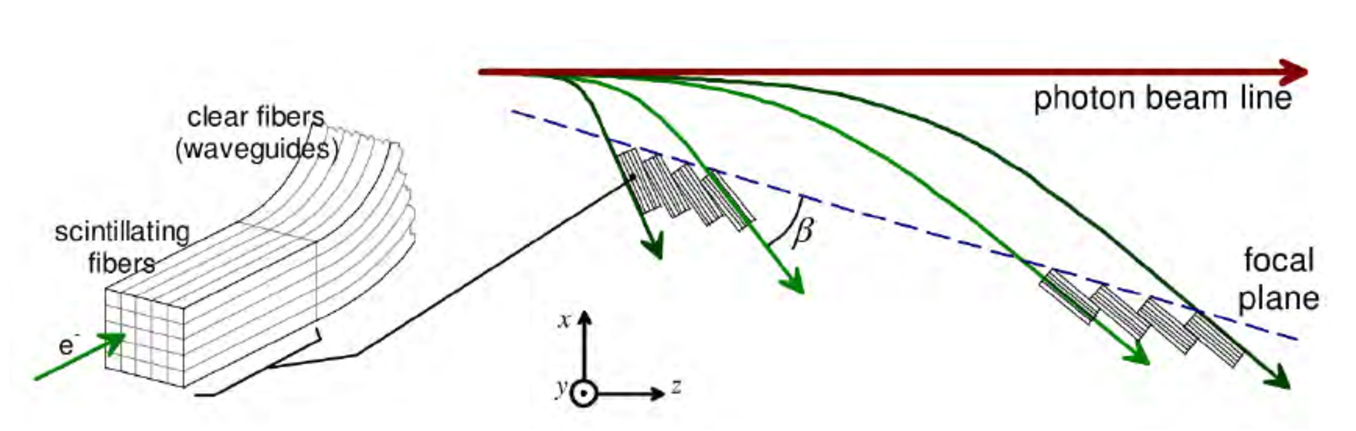
\includegraphics[clip=true,width=0.95\linewidth]{figures/TAGM_conceptual.pdf}
\end{center}
\caption{
Conceptual overview of the tagger microscope design, showing the fiber bundles and
light guides (left), and the orientation of these bundles aligned with the incoming
electron beam direction in the tagger focal plane (right). The variation of the
crossing angle $\beta$ is exaggerated for the sake of illustration.
        }
\label{fig:TAGM_conceptual}
\end{figure}

Because the electron trajectories do not cross the focal plane at right angles, the
fiber array must be staggered along the dispersion direction. A staggering step
occcurs every 6 columns, as illustrated in Fig.~\ref{fig:TAGM_conceptual}. The slight
variation of the crossing angle $\beta$ is taken into account by a carefully adjusted
fan-out that is implemented by small evenly-distributed gaps at the rear ends of 
adjacent 6-column groups (bundles). A total of 17 such bundles comprise the full
Tagger Microscope.

The far ends of the scintillation light guides are coupled to Hamamatsu S10931-050P SiPMs. The SiPMs are mounted on a custom-built two-stage preamplifier board, with 15 SiPMs per board. In addition to the 15 individual signals generated
by each preamplifier, the boards also produce three analog sum outputs, each the sum
of five adjacent SiPMs corresponding to the five fibers in a single column. All 510
SiPMs are individually biased by custom bias control boards, one for every two
preamplifier boards. The control boards connect to the
preamplifiers over a custom backplane, and communicate with the
experimental slow controls system over ethernet. Each control board has the
capability to electronically select between two gain modes for the preamplifiers
on that board:
a low gain mode used during regular tagging operation, and a high gain
mode used for triggering on single-pixel pulses during bias calibration.
Each bias control board manages the control and biasing for two preamplifiers.
The control board also measures live values for environmental parameters
(voltage levels and temperatures) in the TAGM electronics, so that alarms can
be generated by the experimental control system whenever any of these parameters
stray outside predefined limits.

Pulse height and timing information for 122 channels from the TAGM is provided by analog-to-digital converters (ADCs) and time-to-digital converters (TDCs). These 122
signals include the 102 column sums plus the individual fiber signals from
columns 7, 27, 81, and 97. Here, each channel goes through a 1:1
passive splitter, with one output going to an ADC and the other through
discriminators to a TDC. The ADCs are 250-MHz flash ADCs with 12-bit
resolution and a full-scale pulse amplitude of 1 V. The TDCs are based
on the F1 TDC chip \cite{Fischer:2000zu}, with a least-count of 62~ps. Pulse thresholds in both
the ADC and discriminator modules are programmable over the range 1-1000 mV
on an individual channel basis, covering the full dynamic range of the TAGM
front end. The TAGM preamplifier outputs (before splitting) saturate at around
2~V pulse amplitude.

The mean pulse charge in units of SiPM pixels corresponding to a
single high-energy electron varies from 150 to 300 pC, depending on the fiber,
with an average of 220 pC and standard deviation of 25 pC. During calibration,
this yield is measured individually for each fiber by selectively biasing
the SiPMs on each row of fibers, one row at a time, and reading out the column
sums. Once all 510 individual fiber yields have been measured, the bias voltages
within each column are adjusted to compensate for yield variations, so
that the mean pulse height in a given column is the same regardless of which
fiber in the column detected the electron. The ADC readout and discriminator
thresholds are set individually for each column, for optimum efficiency and
noise rejection.

The ADC firmware provides an approximate time for each pulse, in addition to the
pulse amplitude. During offline reconstruction, this time information is used to
associate ADC and TDC pulse information from the same channel, so that a
time-walk correction can be applied to the TDC time. Once this correction
has been applied, a time resolution of 230~ps is achieved for the TAGM.
This resolution is based on data collected at rates on the order of 1~MHz
per column, a factor of 2 lower than the 2.2~MHz peak rate anticipated during
\gx{} 2 running. A brief test above 2~MHz per column allowed visual
inspection of the pulse waveforms from the TAGM, without change in the
pulse shape or amplitude. Given that the readout was designed
to operate at rates up to 4~MHz per column without significant degradation
in performance, the TAGM time resolution should be
substantially unaffected by the increased beam intensity of \GX{} Phase 2.

\subsubsection{Broadband tagging hodoscope}\label{sec:TAGHIntro}
The Tagger Hodoscope (TAGH) consists of 222 scintillator counters distributed over a length of 9.25~m and mounted just behind the focal plane of the tagger magnet.
The function of this hodoscope is to tag the full range of photon energy from 25\% to 97\%
of the incident electron energy. A gap in the middle of that range is left open for the registration of the primary coherent peak by the Tagger Microscope. The geometry of the counters in the
vicinity of the microscope is shown in Fig.\,\ref{fig:beam:BEAM_taggerdetectors}. 
This broad coverage aids in alignment of the diamond radiator and expands the \GX{} physics program reach to photon energies outside the range of the coherent peak.
The coverage of the hodoscope counters in the region below 60\% drops to half,
with substantial gaps in energy between the counters. This was done because
the events of primary interest to \GX{} come from interactions of photons
within and above the coherent peak; 
within and above the coherent peak the coverage is 100\% up to the 97\% $E_0$ cutoff.

Each counter in the hodoscope is a sheet of EJ-228 scintillator, 6 mm thick and
40 mm high. The counter widths vary along the focal plane, from 21~mm near the
end-point region down to 3~mm at the downstream end. The scintillators are
coupled to a Hamamatsu R9800 photomultiplier tube (PMT) via a cylindrical acrylic (UVT-PMMA) light
guide 22.2 mm in diameter and 120 mm long. Each PMT is wrapped in $\mu$-metal
to shield the tube from the fringe field of the tagger magnet.

Each PMT is instrumented with a custom designed active base~\cite{tagh:base},
consisting of a high-voltage divider and an amplifier powered by current
flowing through the divider. The base provides two signal outputs, one going
to a flash ADC and the other through a discriminator to a TDC.
Operating the amplifier with a gain factor of 8.5 allows the PMT to operate at a
lower voltage of 900~V and reduce the PMT anode current, therefore improving
the rate capability. The energy bite of each counter ranges between 8.5 and
30 MeV for a 12 GeV incident electron beam.  Typical rates during production
running are 1 MHz above the coherent peak and 2 MHz per counter below the
coherent peak. The maximum sustainable rate per counter is about 4~MHz.

The counters are mounted with their faces normal to the path of the
scattered electrons in two or three rows slightly downstream of the focal
plane, as shown in Fig.\,\ref{fig:beam:BEAM_taggerdetectors}.
This allows the counters to be positioned without horizontal gaps in
the dispersion direction, enabling complete coverage of the entire
tagged photon energy range.

\begin{figure}[tbp]
\begin{center}
%   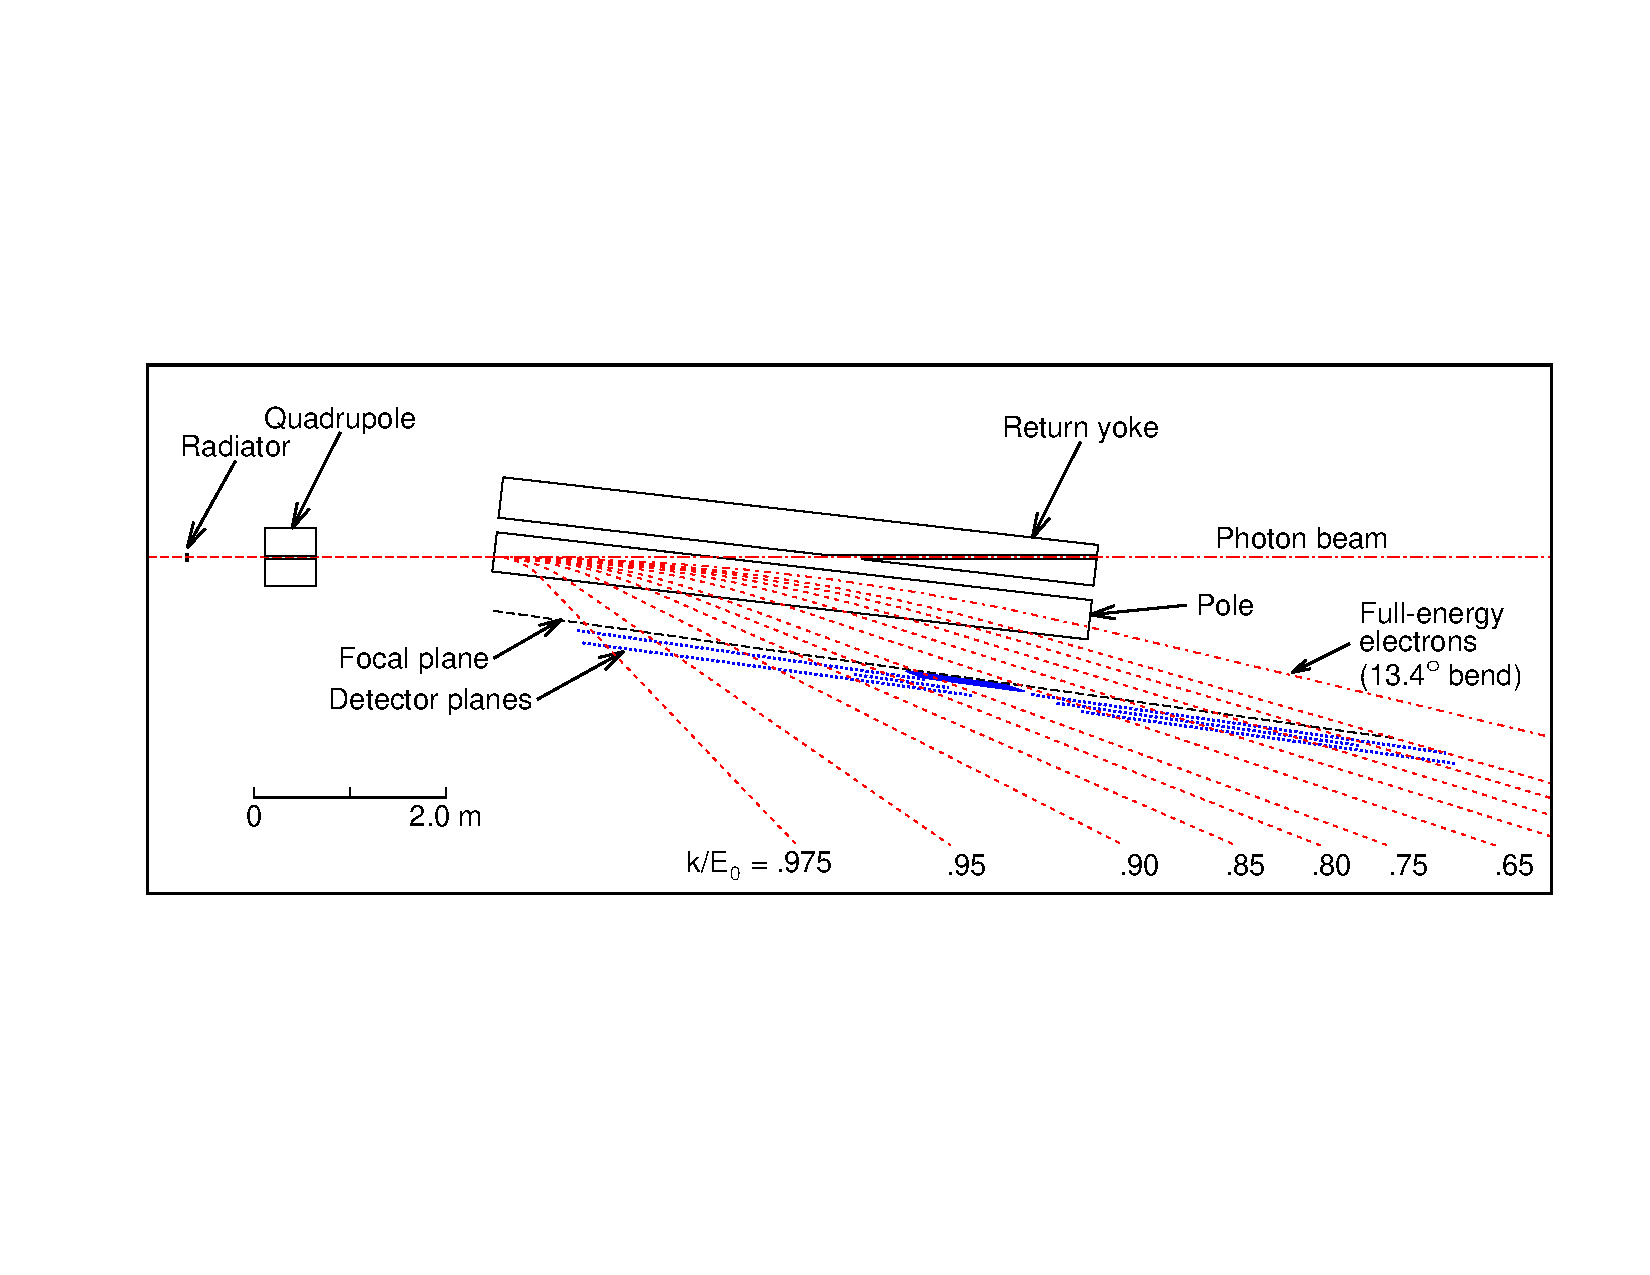
\includegraphics[width=0.95\linewidth]{figures/BEAM_taggerplot.pdf}
%   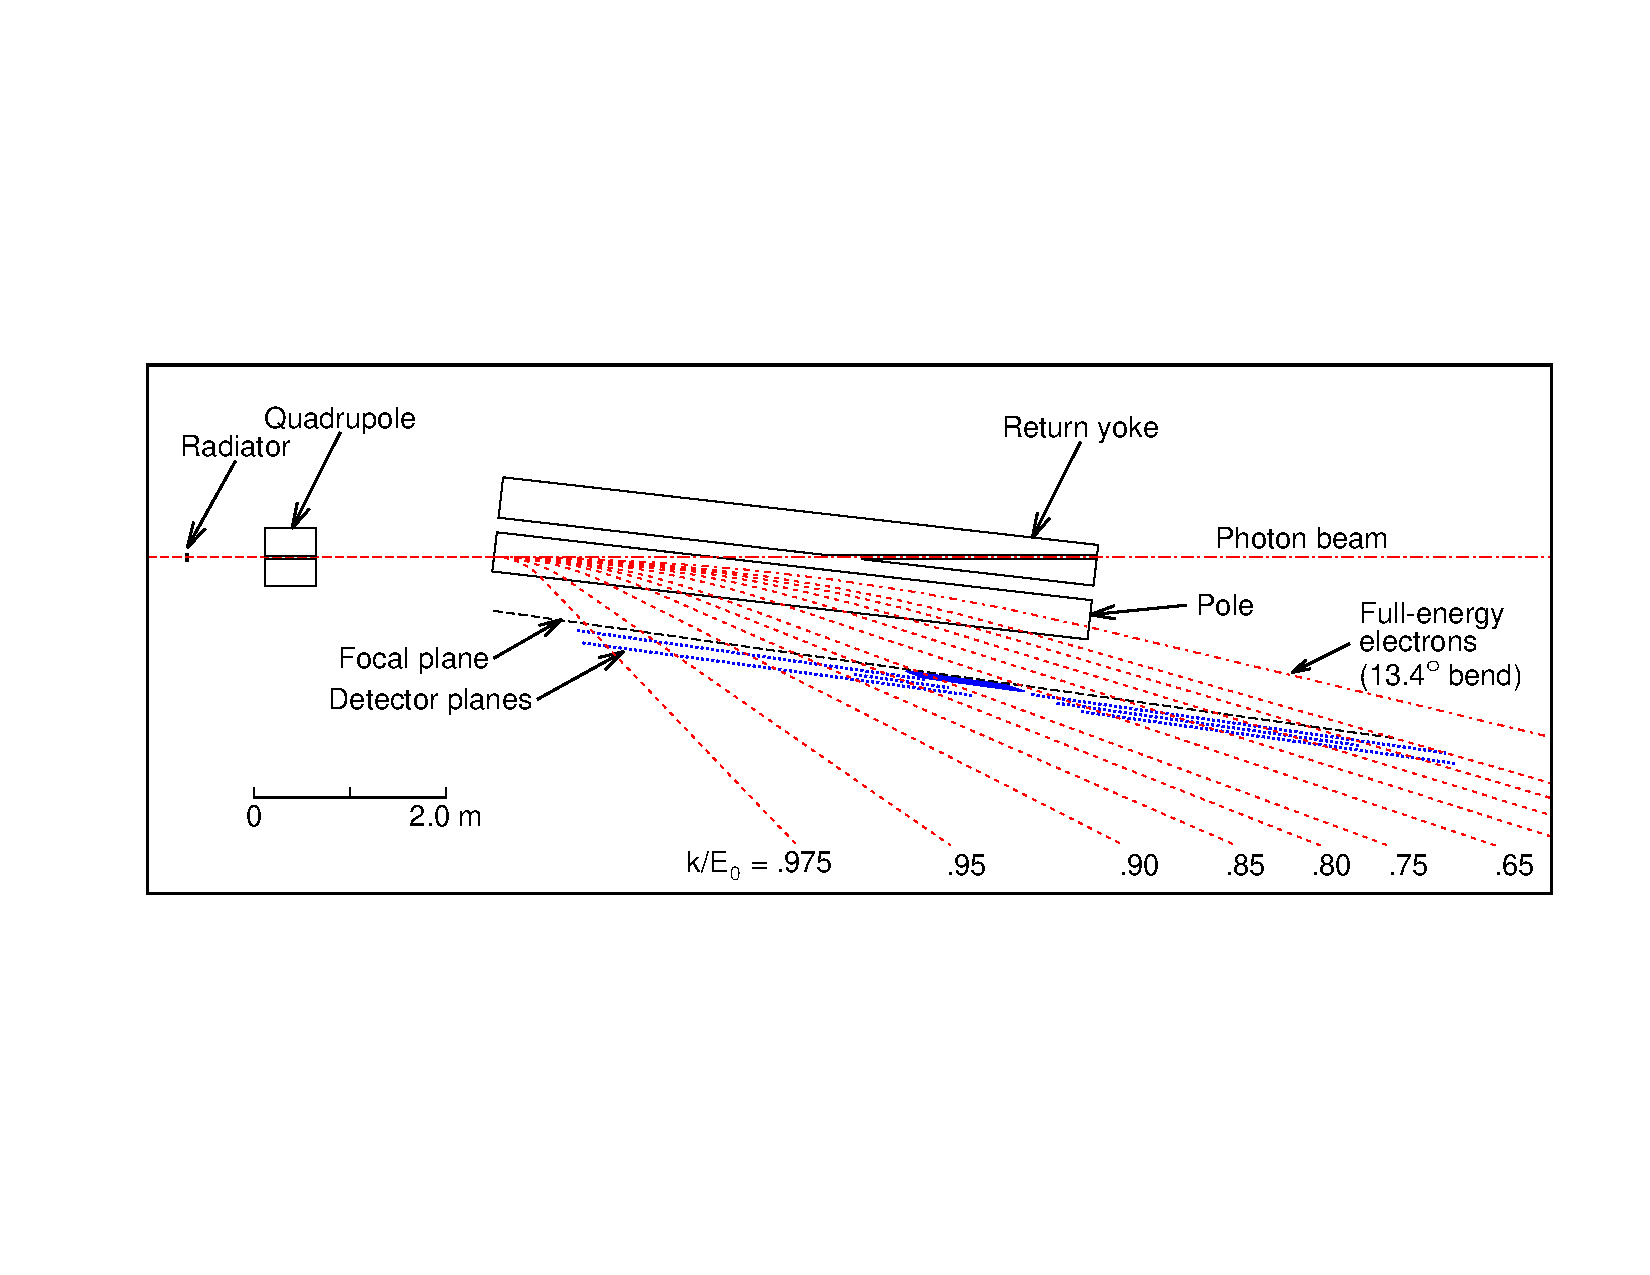
\includegraphics[width=0.95\linewidth,viewport=150 115 628 500]{figures/BEAM_taggerplot.pdf}
      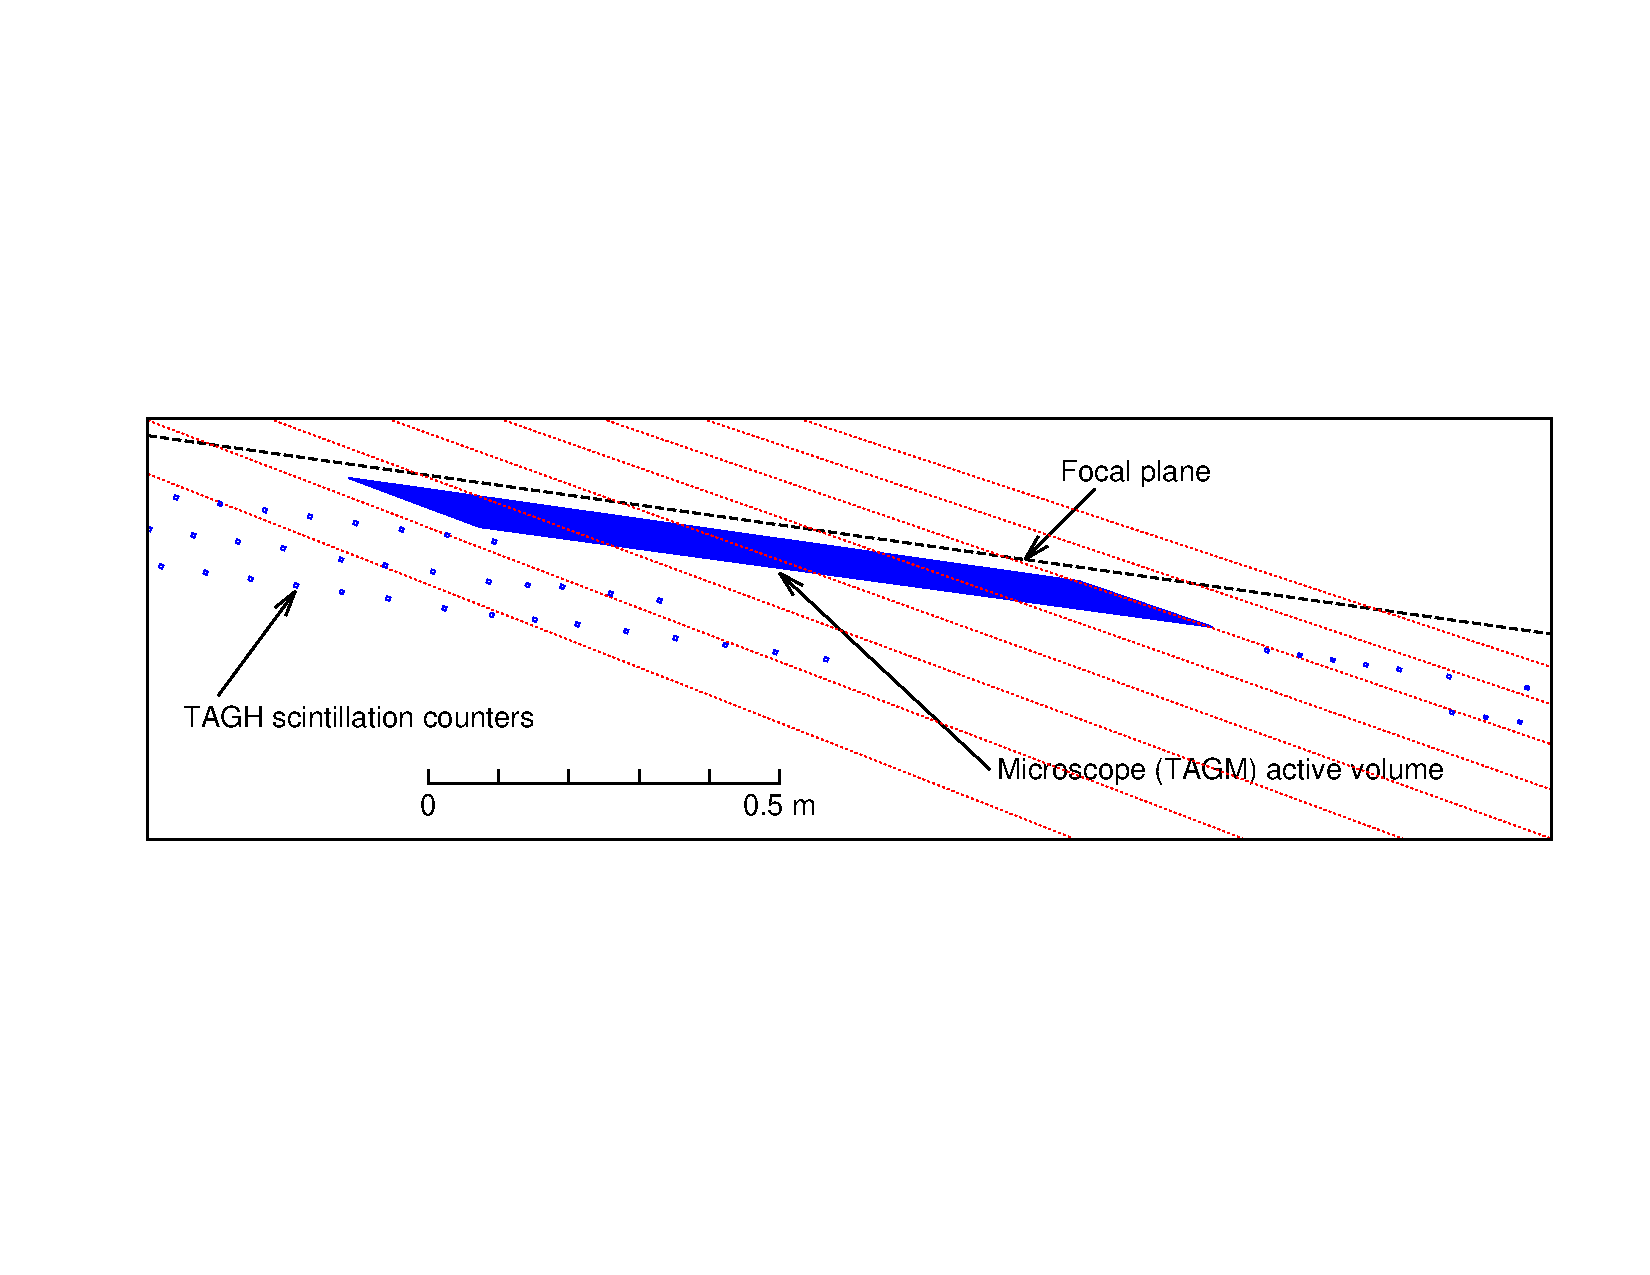
\includegraphics[width=0.95\linewidth,viewport=80 200 750 400]{figures/BEAM_taggerdetectors.pdf}
\caption{Schematic of electron trajectories in the region of the microscope. Shown are the three layers of hodoscope counters on either side of the microscope and the 
               region covered by the microscope.
       \label{fig:beam:BEAM_taggerdetectors}  }

\end{center}
\end{figure}

The mounting frame of the hodoscope is suspended from the ceiling of the Tagger Hall
to provide full flexibility for positioning TAGH. The frame is constructed
to also support the addition of counters to fill in the energy range currently
occupied by the microscope when the TAGM location is changed.

A similar procedure to that described in Section\,\ref{sec:TAGM} for the TAGM is used to apply
a time-walk correction to the TDC times from the TAGH counters. Once this
time-walk correction
is applied, the time resolution of the TAGH is 200~ps. No significant
degradation of this resolution is expected at the operating rates planned
for Phase 2 running, which are on the order of 2 MHz per counter above
the coherent peak. Under these conditions, the rates in the TAGH counters
below the coherent peak would average around 4~Mhz, which is at the top
of their allowed range. These counters will be turned off when
running at full intensity.

\subsection{Tungsten keV filter}

To reduce the photon flux in the $10-100$~keV range, a $100$~$\mu$m tungsten ($3\%$ of a radiation length) foil was installed in the beam line at the entrance of the collimator cave.  We have studied the effect of different foil materials on the anode currents and  random hits in the drift chambers (see Section\,\ref{sec:tracking}), as these factors limit the high-intensity operation of the experiment. By comparing the effect of different materials (Al, Cu, W) with fixed radiation lengths (see Fig.\ref{fig:attenuation})  we learned that the drift chambers are mostly affected by photons in the 70-90 keV range. The analysis of the pulse shape  of the random hits in the CDC confirmed that these photons directly produce hits in the inner layers of the chamber. The insertion of the tungsten foil reduced the number of random hits in the inner CDC layers by a factor of up to 8 and the anode current by $55\%$. The reduction of the current in the FDC was more moderate, about $25\%$. Note that the FDC sense wires are as close as $3$~cm to the beam, while in the CDC the closest wires are at $10$~cm.

\begin{figure}[tbp]
\begin{center}
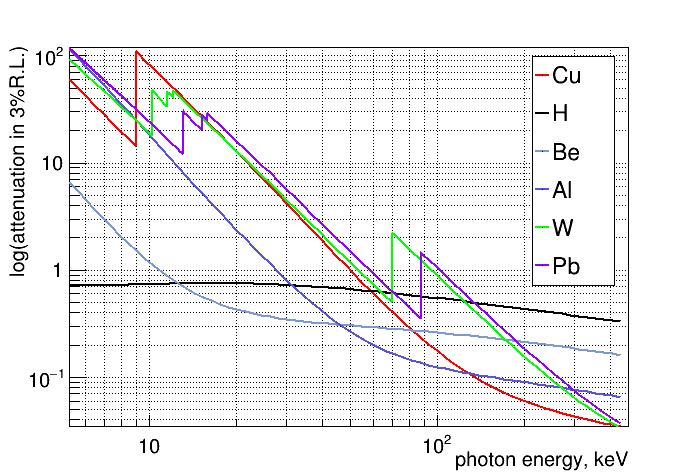
\includegraphics[width=0.5\linewidth]{figures/Attenuation.png}
\caption{Attenuation of low-energy photons in foils with a thickness of  $3\%$ of a radiation length for different materials as a function of photon energy. The W foil was selected to reduce the random background hits in the detector drift chambers.
\label{fig:attenuation}  }
\end{center}
\end{figure}


\subsection{Beam profiler}
The beam profiler is located immediately upstream of the collimator (see Fig.\,\ref{fig:beam:Draw_beamline}) and is
used to measure the photon beam intensity in a plane normal to the incident
photon beam. The profiler consists of two planes
of scintillating fibers, giving information on the photon beam profile
in the X and Y projections. Each plane consists of 64 square fibers,
2 mm in width, read out by four 16-channel multi-anode PMTs. The beam profiler
is only used during beam setup until the photon beam is centered on the active collimator.

\subsection{Active collimator \label{sec:coll}}
The active collimator monitors the photon beam position and provides
feedback to micro-steering magnets in the electron beamline, for the
purpose of suppressing drifts in photon beam position. 
The
design of the active collimator for \GX{} is based on a device 
developed at SLAC for monitoring
the coherent bremsstrahlung beam there \cite{Miller:1973yi}.
The \GX{} active collimator is located on
the upstream face of the primary collimator, and consists of a dense
array of tungsten pins attached to tungsten base plates. The tungsten
plate intercepts off-axis beam photons before they enter the collimator,
creating an electromagnetic shower that cascades through the array
of pins. High-energy delta rays created by the
shower in the pins (known as ``knock-ons") 
are emitted forward into the primary collimator. The resulting net current between the tungsten plates and the collimator is proportional to the intensity of the photon beam on the plate.
The tungsten plates are mounted on an insulating support, and the plate
currents are monitored by a preamplifier with pA sensitivity. 

The tungsten plate is segmented radially into two rings, and each ring is
segmented azimuthally into four quadrants. The asymmetry of the induced 
currents on the plates in opposite quadrants indicates the degree of
displacement of the photon beam from the intended center position. Typical
currents on the tungsten sectors are at the level of 1.4~nA (inner ring)
and 0.85~nA (outer ring) when running with a 50~$\mu$m diamond crystal
and a 200-nA incident electron beam current. The current-sensitive preamplifiers
used with the active collimator are PMT-5R devices manufactured by
ARI Corporation\footnote{Advanced Research Instruments Corporation, http://aricorp.com.}. The PMT-5R has six remotely selectable gain settings
ranging from $10^{12}$~V/A to $10^6$~V/A, selectable by powers of 10.
This provides an excellent dynamic
range for operation of the beam over a wide range of intensities, from
1~nA up to several $\mu$A. The preamplifier input stage exhibits a fixed
gain-bandwidth product of about 2~Hz-V/pA which limits its bandwidth at
the higher gain settings, for example 2~Hz at $10^{12}$~V/A, 20~Hz at
$10^{11}$~V/A.

In-situ electronic noise on the individual wedge currents is measured to
be 1.5~pA/$\sqrt{\mbox{Hz}}$ on the inner ring, and 15~pA/$\sqrt{\mbox{Hz}}$
on the outer ring. The sensitivity of the current asymmetry to position is
0.160/mm for the inner ring and 0.089/mm for the outer. 
With a 50~micron diamond and 200~nA beam current, operating the active
collimator at a bandwidth of 1~kHz yields a measurement error in the
position of the beam centroid of 150~$\mu$m for the inner ring and
450~$\mu$m for the outer ring.
The purpose of the outer ring is to help locate the beam when the beam location
has shifted more than 2~mm from the collimator axis, where the response
of the inner ring sectors becomes nonlinear.

The maximum deviation allowed for the Hall D photon beam position 
relative to the collimator axis is 200~$\mu$m. The active collimator
readout was designed with kHz bandwidth so that use in a
fast feedback loop would suppress motion of the beam at 60~Hz and harmonics
that might exceed this limit. Experience with the Hall-D beam has shown
that the electron beam feedback system already suppresses this motion
to less than 100~$\mu$m amplitude, so that fast feedback using the active
collimator is not required during normal operation. Instead, the active collimator is
used in a slow feedback loop which locks the photon beam position at
the collimator with a correction time constant of a few seconds. This
slow feedback system
is essential for preventing long-term drifts in the photon beam
position that would otherwise occur on the time scale of hours or
days. The active collimator can achieve 200~$\mu$m position resolution down to beam currents as low as 2~nA when operated in this mode with noise averaging over a 5~s interval.

\subsection{Collimator}
The photon beam produced at the diamond radiator contains both incoherent
and coherent bremsstrahlung components. In the region of the coherent peak,
where photon polarization is at its maximum, the angular spread of coherent
bremsstrahlung photons is less than that of incoherent bremsstrahlung.
The characteristic emission angle for incoherent bremsstrahlung is
$m/E = 43$~$\mu$rad at 12~GeV, whereas the coherent flux within the
primary peak is concentrated below 15~$\mu$rad with respect to the beam
direction. Collimation increases the degree of linear polarization in
the photon beam by suppressing the incoherent component relative to the
coherent part.

The Hall-D primary collimator provides apertures of 3.4 mm and 5.0 mm in a
tungsten block mounted on an X-Y table. The 5.0~mm collimator is used
under normal \GX{} running conditions.
The tungsten collimator is surrounded by lead shielding.
The collimator may also be positioned to block the beam to prevent
high-intensity beam from entering the experimental hall during tuning
of the electron beam. Downstream of the primary collimator, a
sweeping magnet and shield wall, followed by a secondary collimator
with its sweeping magnet and shield wall, suppress charged
particles and photon background around the photon beam that are
generated in the primary collimator. The photon beam exiting the
collimation system then passes through a thin pair conversion target. The resulting $e^+e^-$ pairs are used to continuously monitor the photon beam flux and polarization.

\subsection{Triplet Polarimeter \label{sec:tpol}}
The Triplet Polarimeter (TPOL) is used to measure the degree of polarization
of the linearly-polarized photon beam \cite{DUGGER2017115}.
The polarimeter uses the process of $e^+e^-$ pair production on atomic electrons 
in a beryllium target foil, with the scattered atomic electrons
measured using a silicon strip detector.
Information on the degree of polarization of the photon beam is
obtained by analyzing the azimuthal distribution of the scattered
atomic electrons.

\subsubsection{Determination of photon polarization \label{sec:polarization}}
Triplet photoproduction occurs when the polarized photon beam interacts
with the electric field of an atomic electron within a target material
and produces a high energy $e^+e^-$ pair. When coupled with
trajectory and energy information of the $e^+e^-$ pair, the azimuthal
angular distribution of the recoil electron provides a measure of
the photon beam polarization. The cross section for triplet photoproduction
can be written as $\sigma_t = \sigma_0 [ 1 - P \Sigma \cos(2\varphi)]$
for a polarized photon beam, where $\sigma_0$ is the unpolarized triplet
cross section, $P$ the photon beam polarization, $\Sigma$ the beam
asymmetry for the process, and $\varphi$ the azimuthal angle of the
recoil electron trajectory with respect to the plane of polarization
for the incident photon beam. To determine the photon beam polarization,
the azimuthal distribution of the recoil electrons is recorded and fit
to the function $A [ 1- B \cos(2\varphi)]$  where the variables $A$ and
$B$ are parameters of the fit, with $B = P \Sigma$. The value of
$\Sigma$ depends on the beam photon energy, the
thickness of the converter target, and the geometry of the setup.
The value of $\Sigma$ was determined to be $0.1990 \pm 0.0008$ at 9~GeV for the \GX{} beamline
and a 75~micron Be converter~\cite{DUGGER2017115}.

The TPOL detects the recoil electron arising
from triplet photoproduction. 
This system consists of a converter tray and positioning assembly, which holds
and positions a beryllium foil converter where the triplet photoproduction
takes place.  A silicon strip detector (SSD) detects the recoil electron
from triplet photoproduction, providing energy and azimuthal angle information
for that particle. A vacuum housing, containing the pair production target and
SSD, supplies a vacuum environment minimizing multiple Coulomb scattering
between target and SSD. Preamplier and signal filtering electronics are placed
within a Faraday-cage housing.

The preamplifier enclosure is lined with a layer of copper foil to reduce exterior electromagnetic signal interference.
Signals from the downstream (azimuthal sector) side of the SSD are fed to a charge-sensitive preamplifier located outside the vacuum.
In operation, the TPOL vacuum box is coupled directly to the evacuated
beamline through which the polarized photon beam passes. 

Upon entering TPOL, the photon beam passes into the
beryllium converter, triplet photoproduction takes place, an
$e^+e^-$ pair is emitted from the target in the forward direction,
and a recoil electron ejected from the target at large angles with
respect to the beam is detected by the SSD within the TPOL vacuum chamber.
The recoil electron is ejected at large angles and detected by the SSD.
The $e^+e^-$ pair, together with any beam photons that did not
interact with the converter material, pass through the downstream port of
the TPOL vacuum box into the evacuated beamline, which in turn passes
through a shielding wall into the Hall-D experimental area. 
The $e^+e^-$ pair then enters the vacuum box and magnetic field of the \GX{}
Pair Spectrometer, while photons continue through an evacuated beamline to
the target region of the \gx{} detector. Accounting for all sources of
uncertainty from this setup, the total estimated systematic error in
the TPOL asymmetry $\Sigma$ is 1.5\% \cite{DUGGER2017115}.

\subsection{Pair Spectrometer  \label{sec:ps}}
The main purpose of the Pair Spectrometer (PS) \cite{BARBOSA2015376} 
is to measure the spectrum of the
collimated photon beam and determine the fraction of linearly polarized
photons in the coherent peak energy region. The TPOL relies on the PS
to trigger on pairs in coincidence with hits in the recoil detector.
The PS is also used to monitor the photon beam flux, and for 
energy calibration of the tagging hodoscope and microscope detectors.

The PS, located at the entrance to Hall D, %(Fig.~\ref{fig:beam:hall-d}).
reconstructs the energy of a beam photon by detecting
the $e^+e^-$ pair produced by the photon in a thin converter.
The converter used is typically the beryllium target housed within TPOL; 
otherwise the PS has additional converters that may
be inserted into the beam with thicknesses ranging between 0.03\%
and 0.5\% of a radiation length.
The produced $e^+e^-$ leptons are deflected in a modified 18D36 dipole magnet
with an effective field length of about 0.94~m and detected in two
layers of scintillator detectors: a high-granularity hodoscope and
a set of coarse counters, referred to as PS and PSC counters, respectively.
The detectors are partitioned into two identical arms positioned symmetrically on
opposite sides of the photon beam line. The PSC consists of sixteen
scintillator counters, eight in each detector arm. Each PSC counter is
4.4~cm wide and 2~cm thick in the direction along the lepton trajectory
and 6~cm high. Light from the PSC counters is detected using Hamamatsu
R6427-01 PMTs. The PS hodoscope consists of 145 rectangular tiles
(1 mm and 2 mm wide) stacked together. Hamamatsu SiPMs were chosen for
readout of the PS counters
~\cite{Barbosa:2017zzw,Somov:2017kif,Tolstukhin:2014zsa}.

Each detector arm covers an $e^\pm$ momentum range between 3.0 GeV/c
and 6.2 GeV/c,  corresponding to reconstructed photon energies between
6~GeV and 12.4~GeV. The relatively large acceptance of the hodoscope
enables energy determination for photons with energies from below the coherent peak
to the beam endpoint energy near 12~GeV.



The pair energy resolution of the PS hodoscope is about 25 MeV.
The time resolution of the PSC counters is 120~ps, which allows coincidence measurements between the tagging detectors and the PS within an electron beam bunch. Signals from the PS detector are delivered to the trigger system,
as described in Section~\ref{sec:trig}. The typical rate of PS double-arm coincidences
is a few kHz. Details about the performance of the spectrometer are given in~\cite{Somov:2017vhp,Somov:2016bgb}.

%\subsubsection[Spectrometer]{Spectrometer\label{sec:beamline:ps-spetrometer}}

%Layout of the Hall D pair spectrometer is presented in Fig.~\ref{fig:beam:ps-layout}. 
% --------------------------------------------
%\begin{figure}[h]
%\begin{center}
%%   \tikzstyle{background grid}=[draw, black!50,step=.5cm]
%%   \begin{tikzpicture}[show background grid]
%%%   \begin{tikzpicture}[]
%%                  % The above right option is used to place the lower left corner
%%                  % of the image at the (0,0) coordinate. 
%%     \node [inner sep=0pt,above right] 
%%      {\includegraphics[angle=0,width=0.98\linewidth]{figs/ps_layout}};
%%       \node (halla)    at (2.0,0.3) [] {{\color{yellow} \scalebox{1.0}{\large A}}};  
%%       \draw[->,yellow,very thick] (halla) edge [] (3.25,1.75);
%%   \end{tikzpicture}
%   \includegraphics[angle=0,width=0.98\linewidth]{figs/ps_layout}
%\end{center}
%\caption{Pair Spectrometer simplified layout. In reality the detectors 
%         are tilted by 4.7$^\circ$ - perpendicular to the average trajectories.}
%\label{fig:beam:ps-layout} 
%\end{figure}
% --------------------------------------------

%Electron-positron pairs are created by beam photons inside a thin
%converter with a typical thickness ranging between 0.03\% and 0.5\% of
%a radiation length. The choice of the converter thickness depends on
%the photon beam flux. The maximum photon flux for GlueX physics runs
%is expected to be 50~MHz in the coherent peak energy region. Three
%converters with different thicknesses are installed in a movable fork
%that can insert one of them into the photon beam. Produced leptons are
%deflected in a 18D36 dipole magnet with an effective field length of
%about 0.94~m. The magnet was brought from Brookhaven National
%Laboratory and was modified at Jefferson Lab by reducing the pole gap
%from 6 inches to 3 inches. The magnet is operated at a nominal field
%of 1.8~T; the field integral is $\int{}Bdl\approx$1.60~T\,m. The beam
%angular spread is $<0.04$~mrad, and the angular spread of the pair
%production is $\sim{}\gamma^{-1}<0.2$~mrad. The multiple scattering at
%3~GeV in the thickest converter adds about 0.3~mrad. The particle
%deflection by the magnet at the momentum $p$ is
%$\theta{}=0.3\,[\mathrm{GeV/c/T/m}]\int{}Bdl/p$;
%$\theta\approx{}80~\mathrm{mrad}=4.6^\circ$ at 6~GeV.  
%A 1.5~m long vacuum chamber is installed after the magnet.
%Electrons and positrons are registered in two layers of scintillator detectors: a
%high-granularity hodoscope and a set of coarse counters, referred to as PS and PSC, respectively.
%The detectors are organized into two arms positioned symmetrically with
%respect to the photon beam line.  Each detector arm covers a momentum
%range of $e^\pm$ between 3.0 GeV/c and 6.2 GeV/c, corresponding to
%reconstructed photon energies between 6~GeV and 12.4~GeV. Relatively
%large acceptance of the hodoscope allows one to reconstruct photons
%with energies in the coherent peak energy region and also in the range
%near the beam end-point energy of 12~GeV. This can be used for the
%energy calibration of the hodoscope detectors.

%\begin{table}[h]
%  \begin{center}
%    \caption{The coordinates of the inner counters (the edge closest to the beam)
%             with respect to the magnet center. The survey was done at 2-Nov-2015. 
%       \label{tab:beam:ps-ccordinates}
%    }
%    %\vspace{3mm}
%    \begin{tabular}{l|r|r}
%       \hline
%       Detector & $Z$, mm & $X$, mm \\
%       \hline
%       \hline
%       PS~ Right arm & 2928.4 & -238.7 \\
%       PS~ Left~ arm & 2928.3 &  238.3 \\
%       PSC Right arm & 3416.2 & -274.4 \\
%       PSC Left~ arm & 3416.1 & ~274.8 \\
%       \hline
%    \end{tabular}
%  \end{center}
%\end{table}

%\subsubsection[PS: High Resolution Detector]{PS: High Resolution Detector
%  \label{sec:beamline:ps-hresol}
%}
%
%Each arm of the high resolution detector consists of 145 rectangular
%tiles made of EJ-212 scintillator~\footnote{
%  ELJEN Technology Plastic Scintillators \url{http://www.eljentechnology.com}. 
%}, stacked together as
%shown in Fig.~\ref{fig:beam:ps-tiles}. The tile height is 3 cm and the
%length along the particle path in scintillator is 1 cm. Out of 145 tiles,
%40 tiles close to the beam are 1~mm thick, the rest are 2~mm thick.
% The momentum bin size of the tile depends on the electron/positron energy as 
%%$\Delta{}p=\Delta{}x/x\cdot{}p$ 
%and constitutes about 13~MeV/c for 3~GeV and 24~MeV/c for 6~GeV particles.
%Tiles are optically isolated using 10~$\mu$m
%aluminized Mylar foil. This reflective foil also covers the bottom of
%the tile assembly. In order to keep the tiles parallel to the
%particle trajectories, the tiles are organized into 18 groups. Each
%group is tilted by $\sim$0.005~mrad using 0.05~mm thick shims
%(adhesive strips) positioned between the adjacent groups. The 
%first group is tilted by about 80~mrad, so that the tiles are parallel
%the 6~GeV particle trajectories.
%
%Light from a tile is collected using two 20~cm long 2$\times$2~mm$^2$
%double-clad BCF-92 wave-length shifting (WLS) fibers,
%glued to the sides of the tile using BC 600 Optical Cement. A tile
%assembly with two WLS optical fibers is shown in
%Fig.~\ref{fig:beam:ps-tiles}. The peak of the emission spectrum for EJ-212
%%scintillator occurs at the wavelength of 423 nm, which couples well
%with the absorption spectrum of the BCF-92 fiber. Light is
%subsequently re-emitted inside the fiber in the green range with an
%emission peak of 492 nm.
%
%Collected light is transmitted to the end of the WLS fiber. A pair of
%fibers from each tile is inserted into a hole in an aluminum mounting
%plate. %, as shown on the upper plot of Fig.~\ref{fig:hodoscope}. 
%The light detection is performed using Hamamatsu
%surface mount S10931-050P silicon photomultipliers with an effective
%photosensitive area of 3$\times$3~mm$^2$ and a pixel size of 0.05$\times$0.05~mm$^2$.
%These sensors have a photon detection efficiency (PDE) larger
%than 20\% at a wavelength of 500~nm and a typical gain of about
%$7\cdot{}10^5$~\footnote{
% Hamamatsu Corporation, MPPC S10931-050P, 
% \url{http://www.electronicsdatasheets.com/pdf-datasheets/hamamatsu/s10931050p}.
%}.
%Each photo sensor is coupled to two WLS fibers
%from a single tile.
%The electronics board (Fig.~\ref{fig:beam:ps-electr-assemb} left) 
%with 145 SiPMs is attached
%to the mounting plate.
%The SiPMs are arranged in two arrays
%of 3$\times$35 and 5$\times$8 sensors, which are connected to 2~mm and~1 mm
%tiles, respectively. SiPMs are optically isolated using a plastic
%spacer.
%
%
%% --------------------------------------------
%\begin{figure}[h]
%\begin{center}
%   \includegraphics[angle=0,width=0.45\linewidth]{figs/ps_tiles_photo_small}\hspace{0.05\linewidth}%
%   \includegraphics[angle=0,width=0.38\linewidth]{figs/ps_assembly_photo}
%\end{center}
%\caption{Scintillator tiles with two WLS fibers glued to sides of each tile: %30$\times$10$\times$1~mm$^3$ tile (left) 
%         and 30$\times$10$\times$2~mm$^3$  tile (right).
%        }
%\label{fig:beam:ps-tiles} 
%\end{figure}
%% --------------------------------------------
%
%% --------------------------------------------
%\begin{figure}[h]
%\begin{center}
%   \includegraphics[angle=0,width=0.43\linewidth]{figs/ps_sipm_plate_photo}\hspace{0.05\linewidth}%
%   \includegraphics[angle=0,width=0.47\linewidth]{figs/ps_assembly_drawing}
%\end{center}
%\caption{Electronics board with 145 SiPMs (left); 
%         the PS detector assembly (right).
%        }
%\label{fig:beam:ps-electr-assemb} 
%\end{figure}
%% --------------------------------------------

%\subsubsection[PSC: Coarse Resolution Detector]{PSC: Coarse Resolution Detector
%  \label{sec:beamline:ps-coarse} }
%
%Sixteen coarse scintillator counters, eight in each detector arm, are
%positioned about 40~cm behind the hodoscope.  The counters are 4.4~cm
%wide in the direction perpendicular to the particle trajectory, 2~cm
%thick, and 6~cm in height.  Hamamatsu R6427-01 PMTs are used to detect
%the scintillation light. The counters are used to produce a pair
%spectrometer trigger by requiring a coincidence of hits in the two
%detector arms. They also help to reduce background originating from
%interactions of $e^\pm$ inside the magnet pole edges to the level
%below 1\% by constraining the $e^\pm$ trajectories.  Counter rates
%depend on the converter thickness and photon beam flux. The maximum
%rate will not exceed 10~kHz per PSC counter during GlueX operation.
%
%
%\subsubsection[Electronics]{Electronics\label{sec:beamline:ps-electronics}}
%
%The PS hodoscope front end electronics consists of an amplifier and a
%SiPM bias voltage control circuit developed at Jefferson Lab. Signals
%from the SiPMs are amplified using the amplifier with a gain of about
%a factor of 20.  The amplifier is based on commercially available
%devices (operational amplifiers) with 3~GHz bandwidth.  Pulse shaping
%is employed to compensate for the characteristically high SiPM
%capacitance and package inductance. The impulse response shows rise
%and fall times of 3~ns and with trans-impedance gain of 1~mV/$\mu$A.  
%The SiPM operating bias voltage is about 73~V. The
%nominal bias setting is as specified by Hamamatsu (1~V over voltage)
%and fed to the SiPM through a resistive network employing a thermistor
%and a linearizing resistor. The hodoscope control electronics supply
%individually adjusted voltages to groups of 5 SiPM channels; inside
%the group the voltage is adjusted among channels using resistors. The
%thermistor senses the average temperature of closely packed SiPMs in
%thermal equilibrium via a heat spreader PCB layout, thus forming a
%well controlled loop. 
%%The commercially available bias power supply has
%%very low noise characteristics and is well regulated to less than 1~mV
%%long term. The supply allows the user to monitor and adjust the levels
%%as needed and if required. The optimal bias setting will be determined
%%based on experimental conditions.
%
%Signals from both the hodoscope and coarse counters are digitized
%using a twelve-bit multi-channel flash ADC operated at a sampling rate
%of 250~MHz (fADC250-MHz). The PSC counters are also instrumented with
%TDCs, with the intrinsic resolution of $\sim$60~ps.  The timing resolution
%is expected to be better than 200~ps. 
%
%An example of the fADC signal pulse obtained from a PS scintillator
%tile is shown in Fig.~\ref{fig:beam:ps-signals} (left).  The ADC
%sampling time is 4~ns. The SiPMs allow to resolve the number of pixels
%fired, demonstrated in Fig.~\ref{fig:beam:ps-signals} (right). The
%average amplitudes of the signals in the Pair Spectrometer correspond
%to about 60 pixels fired.
%
%%This resolution will allow one
%%to distinguish the electron beam bunch where the bremsstrahlung photon
%%is emitted and therefore relate hits from the pair spectrometer and
%%tagging detectors originating from the same event.
%
%% --------------------------------------------
%\begin{figure}[h]
%\begin{center}
%   \includegraphics[angle=0,width=0.45\linewidth]{figs/ps_sipm_pulse}\hspace{0.05\linewidth}%
%   \includegraphics[angle=0,width=0.45\linewidth]{figs/ps_sipm_pixels_peaks}
%\end{center}
%\caption{PS typical fADC250-MHz signal (left); 
%         PS The spectrum of fADC signals integrated in 60~ns, obtained using a low intensity light source. 
%         The spectrum
%         resolves the peaks from different numbers of pixels fired,
%         including zero (the pedestal) (right).
%        }
%\label{fig:beam:ps-signals} 
%\end{figure}

\subsubsection{Determination of photon flux         \label{sec:ps_flux}}
The intensity of beam photons incident on the \GX{} target is
important for the extraction of cross sections. The photon flux
is determined by converting a known fraction of the photon beam to
$e^\pm$ pairs and counting them in the PS as     a function
of energy. Data from the PS are  collected using a PS trigger, which
runs in parallel to the  main \GX{} physics trigger, as described in
Section~\ref{sec:trig}. The number of beam photons integrated over
the run period is obtained individually for each tagger counter (TAGH
and TAGM), i.e., for each photon beam energy bin. 

The PS calibration parameter used in the flux determination, a product
of the  converter thickness, acceptance, and the detection efficiency
for leptons, is determined using calibration runs with the Total 
Absorption Counter (TAC)~\cite{somov_flux}. The TAC is a small calorimeter
(see Section~\ref{sec:tac}) inserted directly into the photon
beam immediately upstream of the photon beam dump to count the number of beam photons as a function of energy.
These absolute-flux calibration runs are performed at reduced beam intensities in
order to limit the rate of accidental tagging coincidences.
Data are acquired simultaneously from the PS and TAC.
These data enable an absolute flux calibration for the PS
by measuring the number of reconstructed $e^+e^-$ pairs for a given
number of photons of the same energy seen by the TAC. 
Uncertainties on the photon flux determinations are currently being
investigated. The expected precision of the flux determination is on
the level of $1\%$.

\subsection{Total Absorption Counter \label{sec:tac}}
Only a certain fraction of the photons produced at the radiator reach the target and causes an interaction that is seen in the \gx{} detector.
The fraction of tagged photons reaching the \gx{} target is determined as a function of energy from individual TAC coincidence measurements with each tagging counter. These ``tagging fractions'' are  used to scale the counts measured in the PS in order to obtain the total tagged flux that reached the \gx{} target during a given run period.

The TAC is a high-efficiency lead-glass calorimeter, used at low beam currents ($<$ 5nA) to determine the overall normalization of the flux from the \gx{} coherent bremsstrahlung facility.  Using the device at normal \gx{} production currents is not possible, as it would very quickly succumb to radiation damage. Therefore, the TAC is only inserted into the beam during dedicated runs at very low intensities when the detector can run with near 100\% efficiency.
The TAC was originally developed for and deployed in Hall B, for photon beam operations with CLAS \cite{clasnote1992014, clasnote1993011,clasnote1999002}.


%{\color{red} Comment by Stuart: TAC runs have also been performed using v-wires during GlueX phase I, should we mention this?}

%Finally, the photon beam travels through the \GX{} detector, and
%ultimately goes to the photon beam dump just outside the downstream end of the experimental hall.
%The main parameters and properties of the Photon Beam are given in and \ref{tab:operates}.
%{\color{red} Comment by Stuart: Hasn't this already been stated at the beginning of this section?}


%=======================+=========================
%================   Solenoid  ================
%=================================================

\section[Solenoid Magnet]{Solenoid magnet 
  \label{sec:solenoid}
}

\subsection[Overview]{Overview \label{sec:sol:overview}
}

The core of the GlueX spectrometer is a superconducting
solenoid magnet with a bore of about 2~m in diameter and with an overall 
yoke length of about 4.8~m. The photon beam passes along the axis of
the solenoid.  At the nominal current of 1350~A, the magnet provides a magnetic field along the axis of about 2~T.

The magnet was designed and built at SLAC in the early
1970's~\cite{Alcorn-confer-1972} for the LASS
spectrometer~\cite{Aston:1987uc}. The solenoid employs a cryostatically
stable design with cryostats designed to be opened and
serviced with hand tools. The magnet was refurbished and modified%
\footnote{
  The front plate of the flux return yoke was modified, leading to a
  swap of the two front coils and modifications of the return flux
  yoke in order to keep the magnetic forces on the front coil under
  the design limit.  The original gaps between the yoke's rings were
  filled with iron. The Cryogenic Distribution Box was designed and
  built for \gx{}.
} 
for the \gx{} experiment~\cite{Ballard:2011tm, Ballard:2015wma}. 

The magnet is constructed of four separate superconducting coils and
cryo\-stats. The flux return yoke is made of several iron rings.  The
coils are connected in series. A common liquid helium tank is located
on top of the magnet, providing a gravity feed of the liquid to the
coils. The layout of the coil cryostats and the flux return iron
yoke is shown in Fig.~\ref{fig:layout_spectrometer}.
Table~\ref{tab:sol:summary} summarizes the salient parameters of the  magnet.

% ======================================================================================
  

\begin{table}[thp]
 \begin{center}
   \small
   \begin{tabular}{lr}
     \hline
     \hline
       Inside diameter of coils        & 2032 mm \\
       Clear bore diameter             & 1854 mm \\
       Overall length along iron       & 4795~mm \\
       Inside iron diameter            & 2946~mm \\
       Outside iron diameter           & 3759~mm \\
       Original yoke, cast and annealed - steel & AISI 1010 \\
       Added filler plates - steel     & ASTM A36 \\
       Full weight                     & 284~t      \\
       Full number of turns            & 4608 \\
       Number of separate coils        & 4 \\
%       Longitudinal arrangement of coils & 1-2-3-4 & & 2-1-3-4 \\
       Turns per coil 2                &  928 \\   
       Turns per coil 1                & 1428 \\   
       Turns per coil 3                &  776 \\   
       Turns per coil 4                & 1476 \\   
       Total conductor weight          & 13.15 t \\
       Coil resistance at $\sim$300~K & 15.3~$\Omega$ \\   
       Coil resistance at  $\sim$10~K & $\sim$0.15$\Omega$ \\   
       Design operational current      & 1500 A \\
       Nominal current (actual)        & 1350 A \\
       Maximal central field at 1350~A & 2.08 T \\   
       Inductance at 1350~A            & 26.4 H \\
       Stored energy at 1350~A         & 24.1 MJ  \\
       Protection circuit resistor     & 0.061 $\Omega$  \\
%       Total conductor length        & 117600 ft & 35.84 km & {\it same} \\
%       Substrate material            & \multicolumn{1}{r}{Copper} & & {\it same} \\   
%       Copper-to-filament ratio (A)  & \multicolumn{1}{r}{20:1} & & {\it same} \\   
%       Copper-to-filament ratio (B)  & \multicolumn{1}{r}{28:1} & & {\it same} \\   
       Coil cooling scheme             & helium bath \\   
       Total liquid helium volume      & 3200 $\ell$ \\
       Operating temperature (actual)  &  4.5~K \\   
       Refrigerator liquefaction rate at 0~A        & 1.7~g/s    \\
       Refrigerator liquefaction rate at 1350~A     & 2.7~g/s    \\
%       Refrigerator liquefaction rate at 0~A        & 1.7~g\thinspace{}s$^{-1}$    \\
%       Refrigerator liquefaction rate at 1350~A     & 2.7~g\thinspace{}s$^{-1}$    \\
%       Protection circuit limiting voltage & 500 V & & 90 V \\
     \hline
   \end{tabular}
   \normalsize
 \end{center}
  \caption{
    Key parameters of the \gx{} solenoid. The
    coils are listed in order along the beam direction.
    \label{tab:sol:summary}
  }
\end{table}


\subsection[Conductor and Coils]{Conductor and Coils
 \label{sec:sol:coils}
}

The superconductor composite is made of niobium--titanium filaments
%\footnote{The critical temperature is about 10$^\circ$K.} 
in a copper substrate, twisted and shaped into a
$\sim$7.62$\times$1~mm$^2$ rectangular band. The laminated conductor
is made by soldering the superconductor composite band between two
copper strips
%\footnote{Copper CDA 102. Average Resistivity Ratio for
%  300$^\circ$K:4.2$^\circ$K is a minimum of 150:1, claimed by the builders of the
%  magnet\cite{Solen-conductor}. 
%  %It contradicts the data from another
%  %source\cite{CuHandbook}, which specifies $10<$RRR$<100$ for ETP
%  %copper. 
%  Our measurements show RRR$\approx{}$100.
%} 
to form a rectangular cross section of 7.62$\times$5.33~mm$^2$
%\cite{Alcorn-confer-1972}.  
The measured residual resistivity ratio of the conductor at $\sim{}300^\circ{}$K and
$\sim{}15^\circ{}$K is $\approx{}$100.  
%Two types of filaments have
%been used (see Fig.~\ref{fig:sol:conductor-cartoon} and
%Table.~\ref{tab:sol:conductor}). The Grade A conductor provides a higher
%current limit than the Grade B conductor and is used in the area of
%the highest magnetic field (Coil 4).

%The coil was wound on G-10 standoff strips glued on the cylindrical
%inner wall of the liquid helium vessel.  
As the coil was wound, a 0.64~mm-thick stainless steel support band
and two 0.2~mm-thick Mylar insulating strips were wound together with it
for pre-tensioning and insulation%
%(Fig.~\ref{fig:sol:conductor-cartoon})
. 
The liquid helium is in contact with the shorter (5.33~mm) sides of
the cable.

Each of the coils consists of a number of subcoils. Each subcoil
contains a number of ``double pancakes'' with the same number of
turns.
%(see Table~\ref{tab:sol:coils-turns}). 
Each double pancake is made from a single piece of conductor. The
voltage across the subcoils is monitored using special wires passing
through the coils' chimneys along with the helium supply pipes and the
main conductor.

The cold helium vessel containing the coil is supported within the
warm cryostat vacuum vessel by a set of columns designed to provide
sufficient thermal insulation. The columns are equipped with strain
gauges for monitoring the stresses on the columns. The helium vessel
is surrounded by a nitrogen-cooled thermal shield made of copper and stainless-steel panels.
Super-insulation is placed between the vacuum vessel and the nitrogen
shield.  The vacuum vessels are attached to the matching iron rings of
the yoke.

The power supply%
\footnote{Danfysik System 8000 Type 854.}
provides up to 10~V DC for establishing the operating current while ramping. The supply also
includes a protection circuit, which can be engaged by a quench
detector as well as by other signals. During trips, a small dump resistor
of 0.061~$\Omega$ limits the maximum voltage on the magnet to 100~V. The dumping time constant of $L/R \approx 7$~min is
relatively long, but safe according to the original design of the
magnet. A large copper mass and the helium bath are able to absorb a
large amount of energy during a quench without overheating the solder
joints. This permits the use of an ``intelligent''  quench detector with low noise sensitivity and a relatively slow decision time of 0.5~s. The quench detector compares the measured voltages on different subcoils
in order to detect a resistive component.
%The decision is made based on the measured voltages on the
%subcoils.  
While ramping the current, such a voltage is proportional
to the subcoil inductance.  Relative values of inductance of various
subcoils depend on the value of the current because of saturation
effects in the iron yoke. Transient effects are also present at changes
of the slew rate caused by Foucault currents in the yoke.
%The quench detector compares
%voltages on different subcoils in order to detect a resistive
%component that might appear in a subcoil.  
The system includes two redundant detectors: one uses analog signals
and a simplified logic, another is part of the PLC control system (see
Section~\ref{sec:sol:controls}) which uses digitized signals. The PLC
digital programmable device is more sensitive since this monitoring system takes into
account the dependence of the coils' inductance on the current and
provides better noise filtering.  The ramping slew rate is
limited by the transient imbalance of the voltages on subcoils that
may trigger the quench detector. Additionally,
unexplained voltage spikes of 1~ms duration
have been observed in coil 2 at high
slew rates, which can  trigger the quench detector. Powering up the
magnet to 1350~A takes about 8~h.

For diagnostic purposes two 40-turn pickup coils are installed on the bore
surface of the vacuum vessel of each of the coils. 

\subsection[Cooling System]{
   Cooling System
   \label{sec:sol:cryo}
}

The cooling system is described in detail in Ref.~\cite{Lavendure:2014:refrig}.
A stand-alone helium refrigerator located
in a building adjacent to Hall D provides liquid helium and nitrogen
via a transfer line to the Cryogenic Distribution Box above the
magnet. The transfer line delivers helium at 2.6~atm and 6~K to a Joule-Thomson
(JT) valve providing liquid to a cylindrical common helium tank in the
Distribution Box. The level of liquid helium in the tank is measured
with a superconducting wire probe;%
\footnote{
  American Magnetics Model 1700 with HS-1/4-RGD-19"/46"-4LDCP-LL6-S sensor
}
 the liquid level is kept at about half of the tank diameter. The cold helium gas
 from the tank is returned to the refrigerator, which keeps the
 pressure at the top of the tank at 1.2~atm corresponding to about
 4.35~K at the surface of the liquid.%
\footnote{
  The original implementation at SLAC did not recycle the helium and
  operated at atmospheric pressure.
}
Each coil is connected to the common helium tank by two vertical 2-inch
pipes.  One pipe is open at the bottom of the tank while the other one
is taller than the typical level of helium inside the tank. The main
conductor and the wires for voltage monitoring pass through the former
pipe. Additionally, two $\sim$6~m long, 3/8~inch ID pipes go outside
the coil's helium vessel, from the Distribution Box to the bottom of
the coil. One of those pipes, connected to a JT valve in the box, is used to fill the coil initially, but is not used during operation.
The other pipe reaches the bottom of
the common helium tank in order to provide 
a thermo-syphon effect essential
for the proper circulation of helium in the coil. The main current is
delivered into the helium tank via vapor-cooled leads, and is
distributed to the coils by a superconducting cable. After cooling the
leads, the helium gas is warmed and returned to the refrigeration
system. The gas flow through the leads is regulated based on the
current in the magnet; at 1350~A, the flow is about 0.25~g/s. The
coils and the Distribution Box are equipped with various sensors for
temperature, pressure, voltage, and flow rates.

\subsection[Measurements and Controls]{
         Measurements and Controls
        \label{sec:sol:controls}
}

The control system for the superconducting solenoid, power supply, 
and cryogenic system, is based on Programmable Logic
Controllers (PLC)%
\footnote{
  Allen-Bradley Programmable Logic Controllers
  \url{http://ab.rockwellautomation.com/Programmable-Controllers}.
}%
.
The PLC system digitizes the signals from various sensors, communicates with
other devices, reads out the data into a programmable unit for
analysis, and sends commands to various devices. Additionally, the PLC is
connected to EPICS\footnote{Experimental Physics and 
Industrial Control System, https://epics.anl.gov.} in order to display and archive the data (see
Section \ref{sec:controls}).  The practical sampling limit for the readout of the sensor
is a few Hz, which is too low for
detection of fast voltage spikes on the coils due to motion, shorts,
or other effects. Therefore, the voltage taps from the coils
and the pickup coils are read
out by a PXI%
\footnote{
  National Instruments, PXI Platform, \url{http://www.ni.com/pxi/}.
}%
system, which provides a sampling rate of about 100~kHz. The
PXI system also reads out several accelerometers attached to the
coils' chimneys, which can detect motion inside the coils. The PXI
CPU performs initial integration and arranges the data in time-wise
rows with a sampling rate of 10~kHz.  The PLC system reads out the
data from the PXI system. Additionally, the PXI data are read out by
an EPICS server at the full 10~kHz sampling rate and are recorded for further analysis.

\subsection[Field calculation and measurement]{
         Field calculation and measurement
        \label{sec:sol:field}
}

The momentum resolution of the \gx{} spectrometer is larger than
1\% and is dominated by multiple scattering and the spatial
resolution of the coordinate detectors.  Thus, a fraction of a percent is
sufficient accuracy for the field determination.  The coils are
axially symmetric, while the flux return yoke is nearly axially
symmetric, apart from the holes for the coil's chimneys. The field was
calculated using a 2-dimensional field calculator {\it
  Poisson/Superfish}%
\footnote{
   Poisson/Superfish developed at LANL,
   \url{https://laacg.lanl.gov/laacg/services/serv_codes.phtml\#ps}.
} 
, assuming axial symmetry.  The model of the magnet included the
fine structure of the subcoils and the geometry of the yoke
iron. Different assumptions about the magnetic properties of the yoke
iron have been used: the {\it Poisson} default AISI 1010 steel, the
measurements of the original yoke iron made at SLAC, and the 1018
steel used for the filler plates. Since the results of the field
calculations differ by less than 0.1\%, the default {\it Poisson} AISI
1010 steel properties were used for the whole yoke iron in the final
field map calculations.

The three projections of the magnetic field have been measured along lines
parallel to the axis, at four values of the radius and at up to six values
of the azimuthal angle. The calculated field and the measured deviations are shown in Fig.~\ref{fig:sol:field_comparison}. The
tracking detectors occupy the volume of $R<56$~cm and $45<Z<340$~cm. In
this volume the field deviation at $R=0$ does not exceed 0.2\%. The
largest deviation of 1.5\% is observed at the downstream edge of the
fiducial volume and at the largest radius. Such a field uncertainty in
that region does not noticeably affect the momentum resolution. In
most of the fiducial volume the measured field is axially symmetric to
$\approx$0.1\% and deviates from this symmetry by $\approx$2\% at the
downstream edge and the largest radius.

The calculated field map is used for track reconstruction and
physics analyses.
   
% ======================================================================================

%\begin{figure}[tp]
\begin{figure}[!htb]
  \begin{center}
     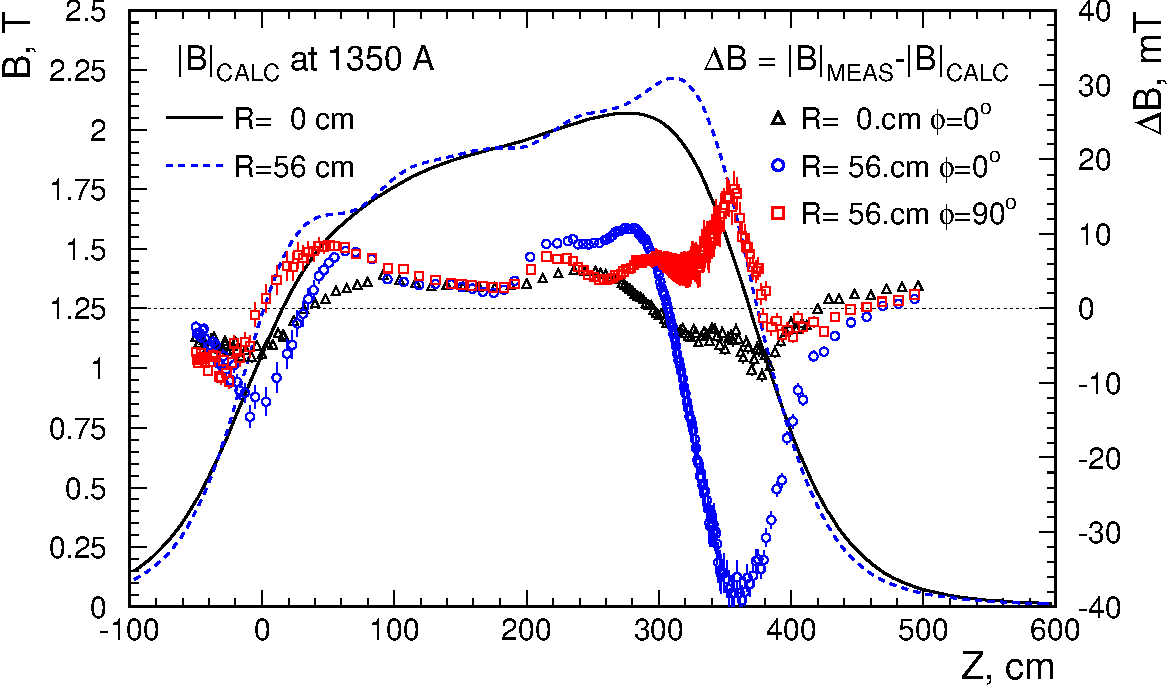
\includegraphics[angle=0,width=1.0\linewidth]{figures/solenoid_field_calc-meas_comparison_7_1_01}%
  \end{center}
  \caption{
    The full field at 1350~A calculated with {\it Poisson} (left
    scale) on the axis and at the edge of the tracking fiducial volume (R=56~cm). The deviations of the measurements from the
    calculations are shown (right scale) on the axis, and at R=56~cm. The measurements were made at 6 azimuthal
    angles. We show the angles (0$^\circ$ and 90$^\circ$) with the largest deviations from the
    calculations.
%    In the area most important for tracking $45<Z<320$~cm the
%    deviations from the calculations are below 0.5\%.
    \label{fig:sol:field_comparison}
  }
\end{figure}


% ----------------------------------------------------------------------

\clearpage   % avoid formatting problems with empty sections
% %=======================+=========================
%================   Detector Overview ================
%=================================================

\section[Detector overview (Curtis)]{Detector overview \label{sec:overview}}
The design of the GlueX detector \cite{Ghoul:2015ifw} is based on a solenoidal magnet that surrounds all detectors in the central region, providing a magnetic field of about $2$~T along the direction of the photon beam, which impinges on a 
$30$~cm-long liquid hydrogen target.  A schematic of the detector including its major sub-detectors is given in Fig.\,\ref{fig:layout_spectrometer}.

% ======================================================================================

\begin{figure*}[!htb]
\centering
  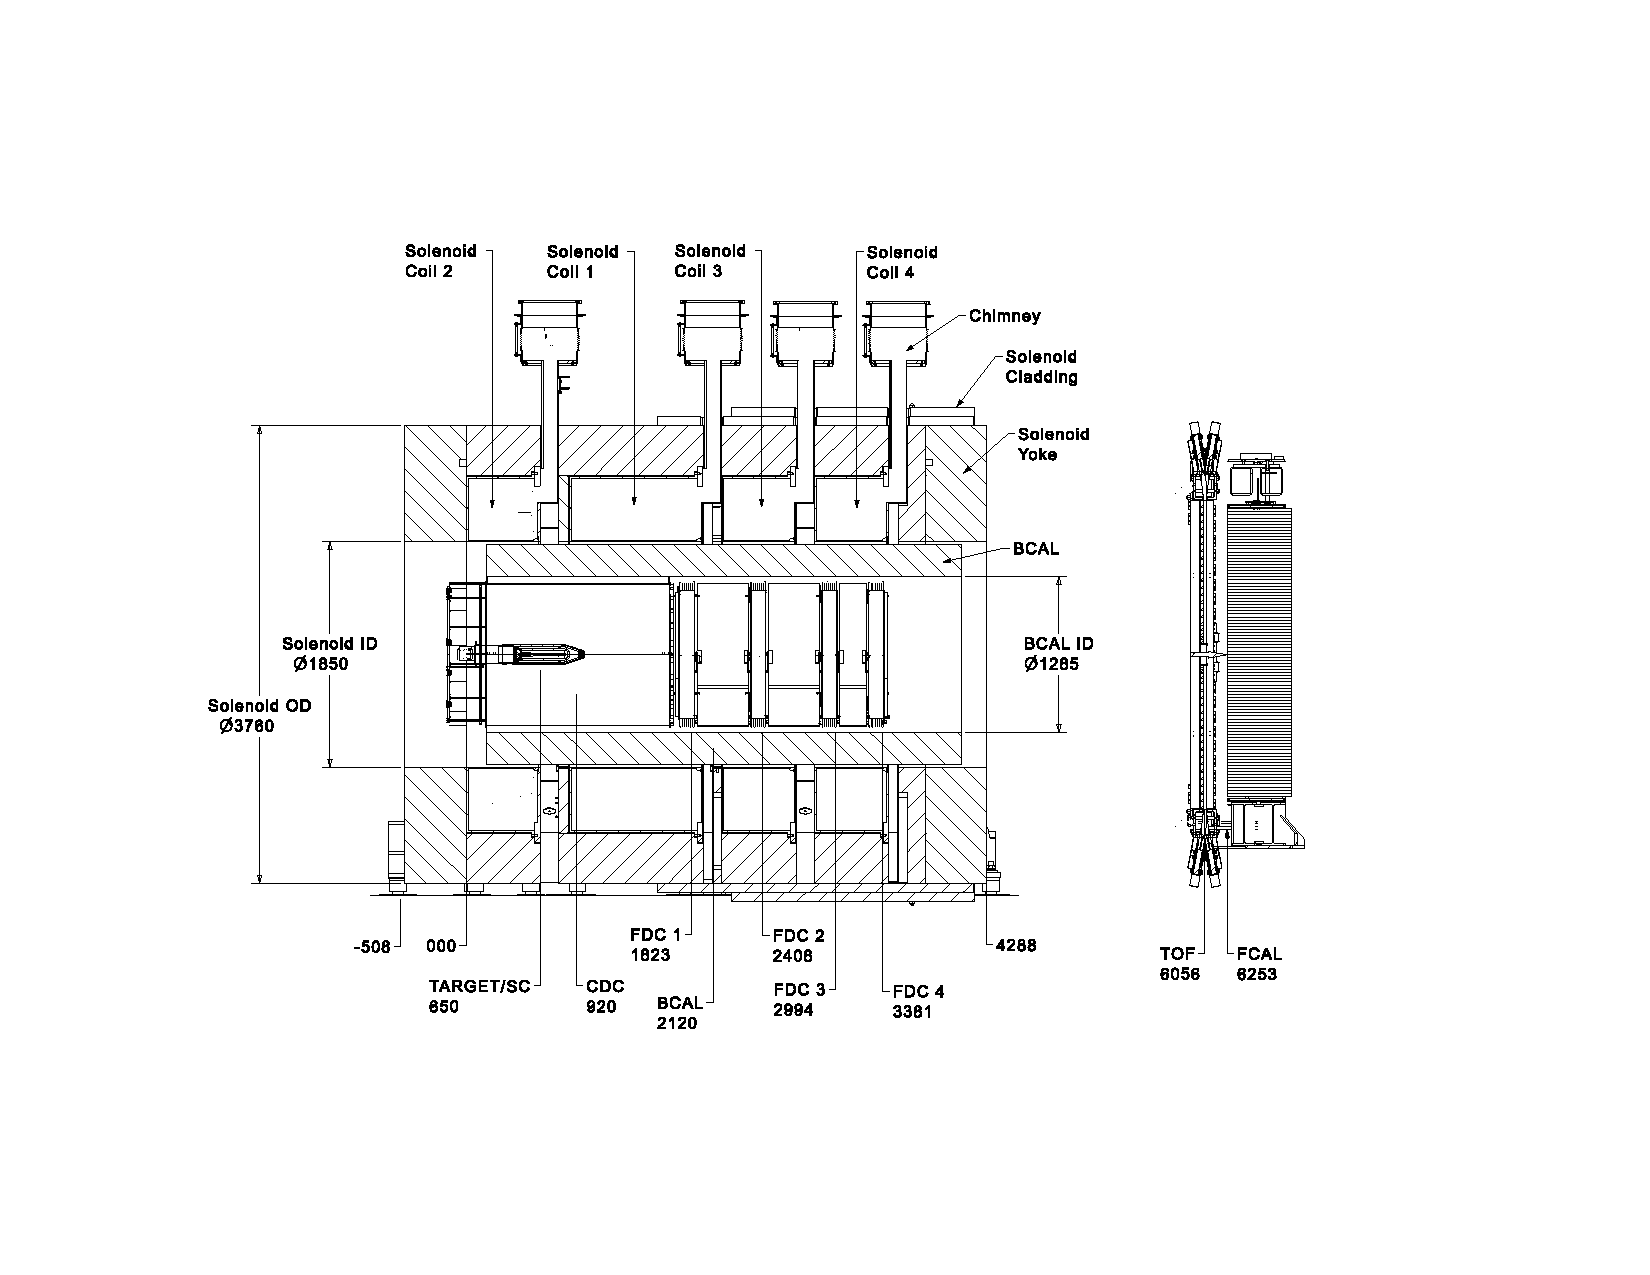
\includegraphics[angle=0,viewport=95 115 628 500,clip,width=1.0\linewidth]{figures/gluex_spectrometer_drawing_01_bw}%
  \caption[layout]{GlueX spectrometer layout. Dimensions are given in mm. The
    numbers show the Z-coordinates of the detectors' centers, or of
    the front face of the calorimeter modules in case of the FCAL.
    Glossary: 
              SC  - Start Counter (Section \ref{sec:st}), 
              CDC - Central Drift Chamber (Section \ref{sec:cdc}), 
              FDC - Forward Drift Chamber (Section \ref{sec:fdc}),
              BCAL - Barrel Calorimeter (Section \ref{sec:bcal}), 
              TOF -  Time-of-Flight hodoscope (Section \ref{sec:tof}), 
              FCAL - Forward Calorimeter (Section \ref{sec:fcal}).
%
%    \begin{tabular}{lll}
%       Name  & Detector & Section \\ \hline
%              SC  & Start Counter & \ref{sec:st} \\ 
%              CDC & Central Drift Chamber  & \ref{sec:cdc} \\ 
%              FDC & Forward Drift Chamber  & \ref{sec:fdc} \\ 
%              BCAL & Barrel Calorimeter    & \ref{sec:bcal} \\ 
%              TOF &  Time-of-Flight hodoscope & \ref{sec:tof} \\ 
%              FCAL & Forward Calorimeter    & \ref{sec:fcal} \\ 
%    \end{tabular}
    \label{fig:layout_spectrometer}
  }
\end{figure*}

% ======================================================================================

%\begin{figure}[tbp]
%\begin{center}
%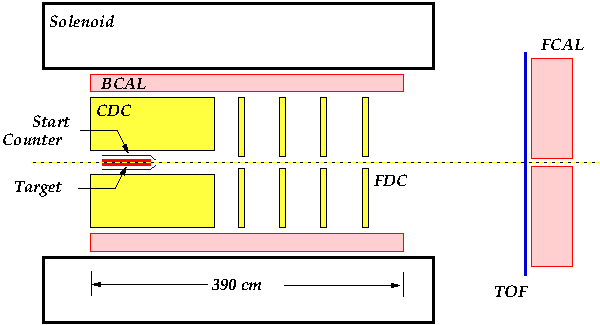
\includegraphics[width=0.7\textwidth]{figures/GlueX_Sketch.pdf}  
%\caption{\label{fig:gluexsketch}          
%  Sketch of GlueX detector.  The main systems of the detector are the Start %Counter \cite{Pooser:2019rhu}, the Central Drift Chamber (CDC) %\cite{VanHaarlem:2010yq} the Forward Drift Chamber (FDC) \cite{Pentchev2017281}, %a scintillator-based Time of Flight (TOF) wall and a lead-glass Forward %Calorimeter (FCAL) \cite{MORIYA201360}. The Barrel Calorimeter (BCAL) is %sandwiched between the drift chambers and the inner radius of the solenoid.  %(Color online)
%}   
%\end{center}  
%\end{figure}

\section[Target]{Target \label{sec:target} }
A schematic diagram of the \gx{} liquid hydrogen cryotarget is shown in Fig.~\ref{fig:Target}. The major components of the system are a pulse tube cryocooler,\footnote{Cryomech model PT415.} a condenser, and a target cell.  These items are contained within an aluminum and stainless steel `L'-shaped vacuum chamber with an extension of closed-cell foam\footnote{Rohacell 110XT, Evonik Industries AG.} surrounding the target cell. In turn, the \gx{} Start Counter (Sec.~\ref{sec:st}) surrounds the foam chamber and is supported by the horizontal portion of the vacuum chamber. Polyimide foils, 100~$\mu$m thick, are used at the upstream and downstream ends of the chamber as beam entrance and exit windows. The entire system, including the control electronics, vacuum pumps, gas-handling system, and tanks for hydrogen storage, are mounted on a small cart that is attached to a set of rails for insertion into the \gx{} solenoid.  To satisfy flammable gas safety requirements, the system is connected at multiple points to a nitrogen-purged ventilation pipe that extends outside Hall D.
\begin{figure*}
\begin{center}
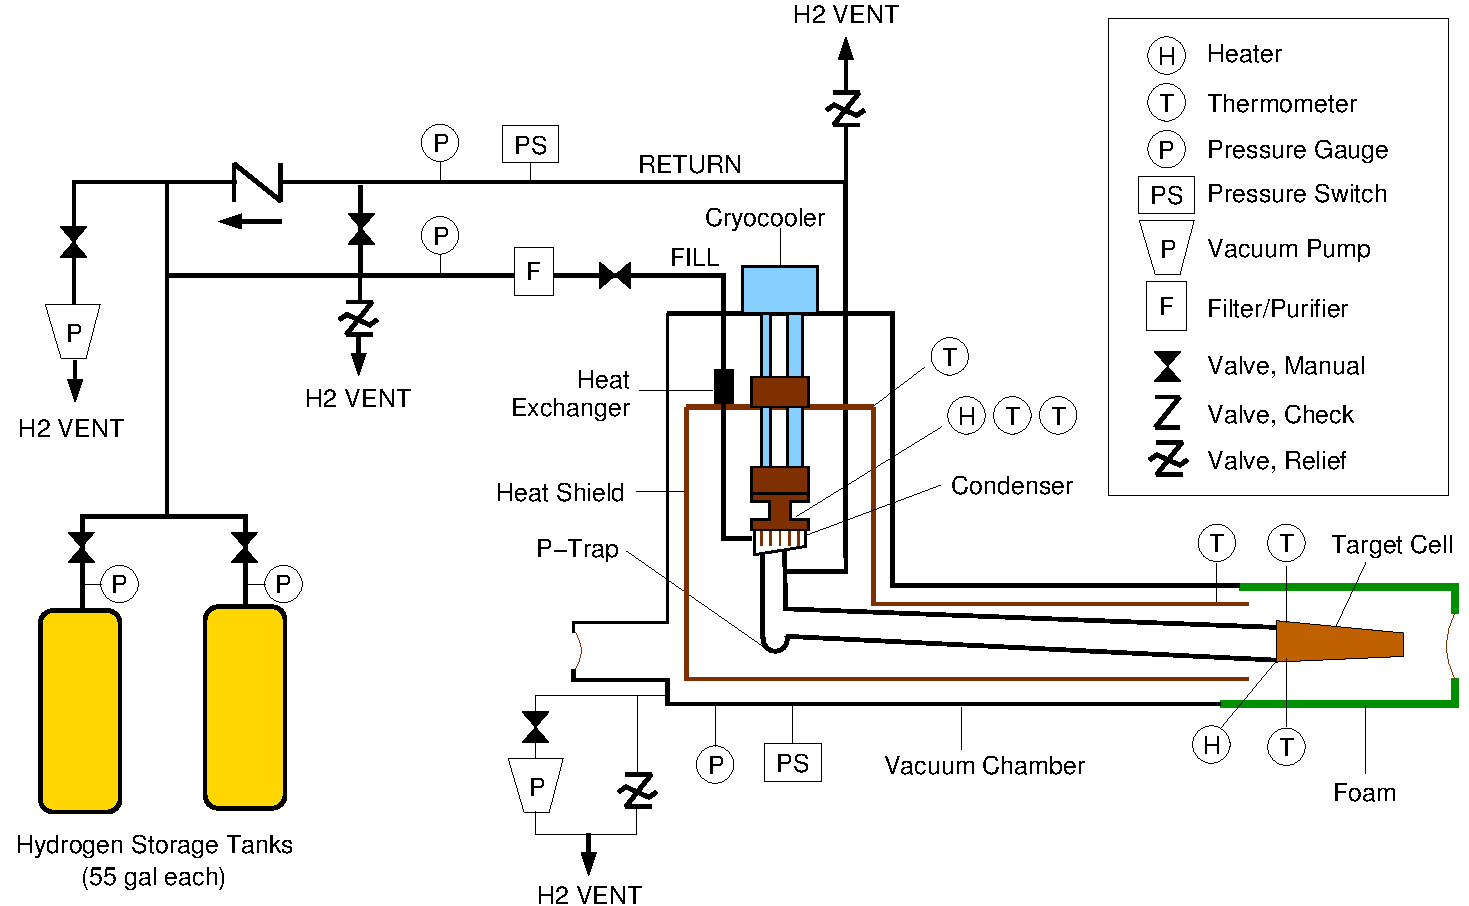
\includegraphics[width=4.5in]{figures/TargetSchematic3.pdf}
\end{center}
\caption{Simplified process and instrumentation diagram for the GlueX liquid hydrogen target (not to scale).
In the real system, the P-trap is above the level of the target cell and is used to
promote convective cooling of the target cell from room temperature.}
\label{fig:Target}
\end{figure*}

Hydrogen gas is stored inside two 200~l tanks and
is cooled and condensed into a small copper and stainless steel container,
the condenser, that is thermally anchored to the second cooling stage of the cryocooler. 
The first stage of the cryocooler is used to
cool the H$_2$ gas to about 50~K before it enters the condenser.
The first stage also cools a copper thermal shield that surrounds all
lower-temperature components of the system except for the
target cell itself, which is wrapped in a few layers of aluminized-mylar/cerex insulation.

The condenser is comprised of a copper C101 base
sealed to a stainless steel can with an indium O-ring.  Numerous vertical 
fins are cut into the copper base, giving a large surface area for condensing hydrogen gas.
A heater and a pair of calibrated Cernox thermometers\footnote{Cernox, Lake Shore Cryotronics.}
are attached outside the condenser, and are used to regulate the heater temperature when the
system is filled with liquid hydrogen.

The target cell, shown in Fig.~\ref{fig:TargetCell}, is similar to
designs used in Hall B at JLab~\cite{HAKOBYAN2008218}.  
The cell walls are made from 100-$\mu$m-thick aluminized
polyimide sheet wrapped in a conical shape and glued along the edge,
overlapping in a 2~mm wide scarf joint.  
The conical shape prevents bubbles from collecting inside the cell, while the
scarf joint reduces the stress riser at the glue joint.  This conical
tube is glued to an aluminum base, 
along with stainless steel fill and return tubes leading to the condenser, a feed-through for two calibrated Cernox thermometers inside the cell, and a
polyamide-imide support for the reentrant upstream beam window.  
Both the upstream and downstream beam
windows are made of non-aluminized,
100~$\mu$m thick polyimide films that have been extruded into the
shapes indicated in Fig.~\ref{fig:TargetCell}. These windows are clearly
visible in Fig.~\ref{fig:z-vertex} where reconstructed vertex positions are shown. All items are glued together using
a two-part epoxy\footnote{3M Scotch-Weld epoxy adhesive DP190 Gray.}
that has been in reliable use at cryogenic temperatures for long periods. 
A second  heater, attached to the aluminum base,
is used to empty the cell for background measurements.
The base is attached to a kinematic mount, which is in turn
supported inside the vacuum chamber using a system of carbon fiber rods.    
The mount is used to correct the pitch and yaw
of the cell, while $X$, $Y$, and $Z$ adjustments 
are accomplished using positioning screws on the target cart. 


During normal operation, a sufficient amount of hydrogen gas is condensed from the storage tanks
until the target cell, condenser, and interconnecting piping are filled with liquid hydrogen
and an equilibrium pressure of about 19~psia is achieved.  
The condenser temperature is regulated at 18~K, while the
liquid in the cell cools to about 20.1~K. The latter temperature is 1~K below the saturation
temperature of H$_2$, which eliminates boiling within the cell and permits a more
accurate determination of the fluid density, 
$71.2 \pm 0.3$~mg/cm$^3$.  
The system can be cooled from room temperature and filled with liquid hydrogen in
approximately six hours.  Prior to measurements using an empty target cell, the liquid hydrogen is boiled back into the storage tanks in about five minutes.  H$_2$ gas continues to condense and drain towards the target cell, but the condensed hydrogen is immediately 
evaporated by the cell heater.  In this way, the cell does not warm above 40~K and
can be re-filled with liquid hydrogen in about twenty minutes.

\begin{figure}
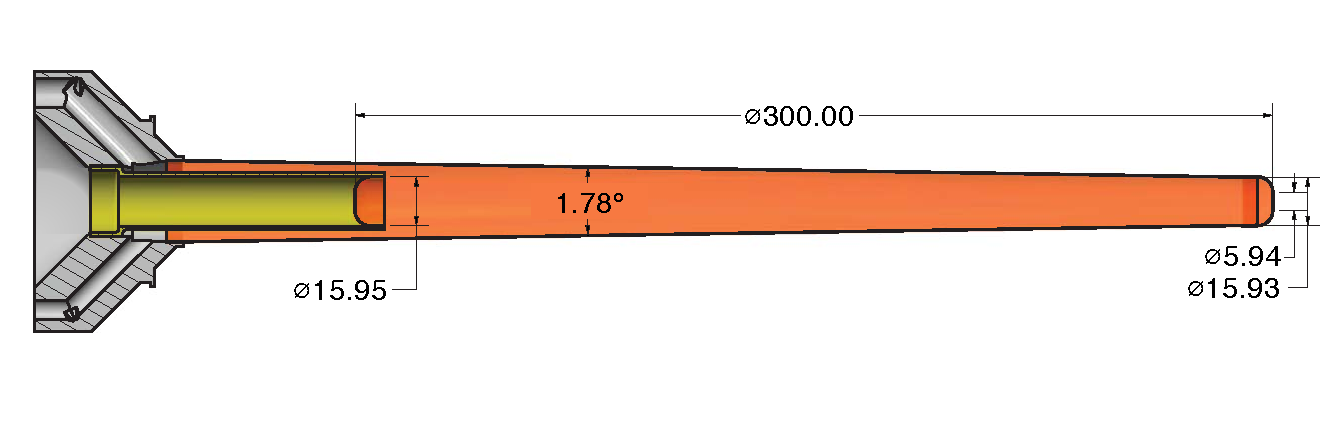
\includegraphics[width=3.5in]{figures/GluexCell_mm.pdf}
\caption{Target cell for the liquid hydrogen target.  Dimensions are in mm.  }
\label{fig:TargetCell}
\end{figure}

Operation of the cryotarget is highly automated, requires minimal user intervention,
and has operated in a very reliable and predictable manner throughout the
experiment. 
The target controls\footnote{The control logic uses National Instruments CompactRIO 9030.} are handled by a LabVIEW program, 
while a standard EPICS softIOC running in Linux provides a
bridge between the controller and JLab's EPICS enviroment (see Section\,\ref{sec:controls}).     
Temperature read back and control of the condenser and target cell thermometers
are managed by a four-input temperature
controller\footnote{Lake Shore Model 336.} with PID control loops of 50 and 100~W.
Strain gauge pressure sensors measure the fill and return pressures with 0.25\% 
accuracy.  When filled with subcooled liquid, 
the long-term temperature ($\pm 0.2$~K) and pressure ($\pm 0.1$~psi)
stability of the liquid hydrogen enable a determination of the density to better than 0.5\%.



\section{Tracking detectors \label{sec:tracking}}
\subsection[Central drift chamber]{Central drift chamber \label{sec:cdc}}

The Central Drift Chamber (CDC) is a cylindrical straw-tube drift chamber which is used to track charged particles by providing position, timing and energy loss measurements~\cite{VanHaarlem:2010yq,GlueXCDCNIM}.
It is situated inside the Barrel Calorimeter, surrounding the target and Start Counter. 
The active volume of the CDC is traversed
by particles coming from the target with polar angles between $6^{\circ}$ and $168^{\circ}$, with optimum 
coverage for polar angles between $29^{\circ}$ and $132^{\circ}$.  
The CDC contains 3522 anode wires of 20~$\mu$m diameter gold-plated tungsten inside Mylar\footnote{www.mylar.com} straw tubes of diameter 1.6~cm in $28$ layers,
located in a cylindrical volume which is 1.5~m long, with an inner radius of 10~cm and outer radius of 56~cm, as measured from the beamline.  
Readout is from the upstream end. 
Fig.\,\ref{fig:CDC_schematic} shows a schematic diagram of the detector.

\begin{figure}[tbp]
\begin{center}
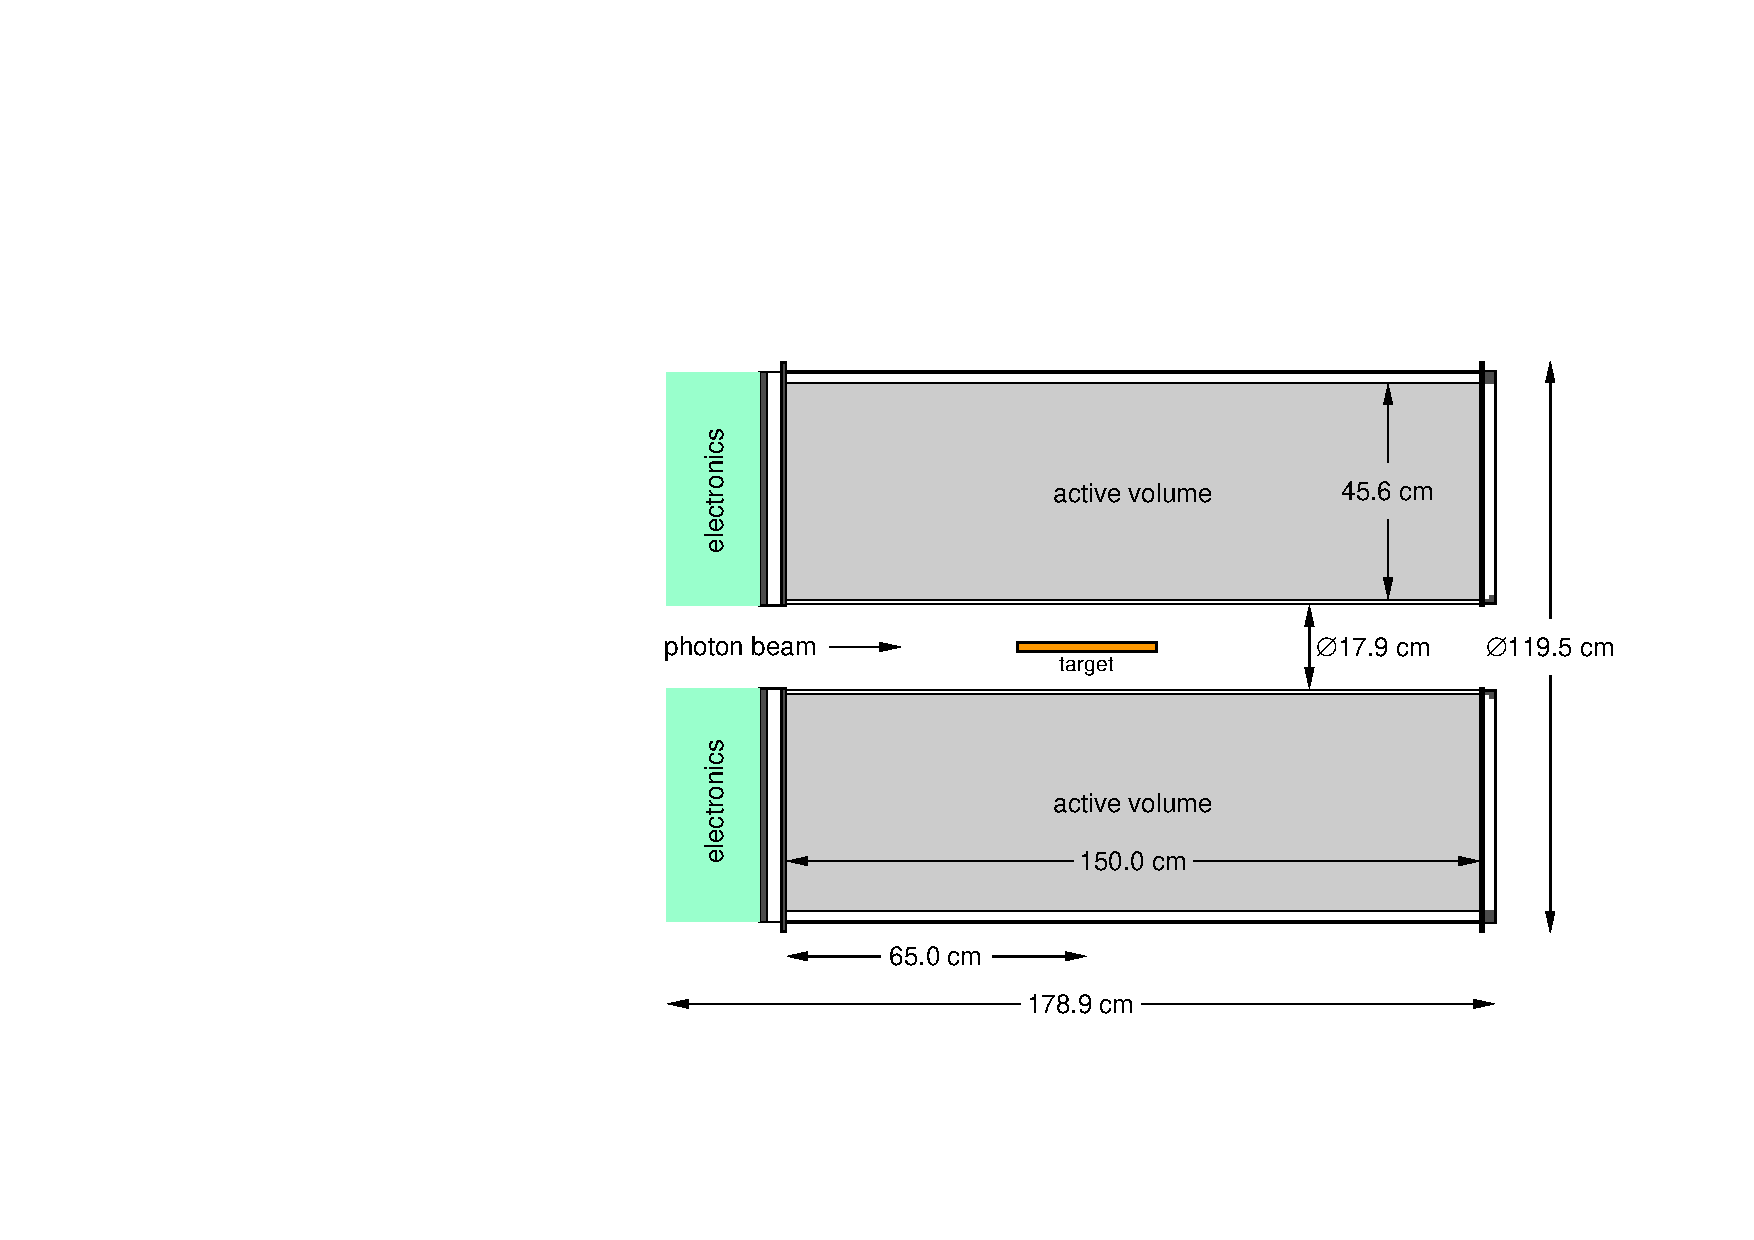
\includegraphics[width=0.7\textwidth]{figures/CDC_schematic.pdf}  
\caption{\label{fig:CDC_schematic}          
  Cross-section through the cylindrically symmetric Central Drift Chamber, along the beamline.}  
\end{center}
\end{figure}

The straw tubes are arranged in 28 layers; 12 layers are axial and 16 layers are at stereo angles of $\pm 6^{\circ}$ to provide position information along the beam direction.
The stereo angle was chosen to balance the extra tracking information provided by the unique combination of stereo and axial straws along a trajectory against the size of the unused volume inside the chamber at each transition between stereo and axial layers. 
Fig.\,\ref{fig:CDC_stereotubes} shows the CDC during construction. 

\begin{figure}[tbp]
\begin{center}
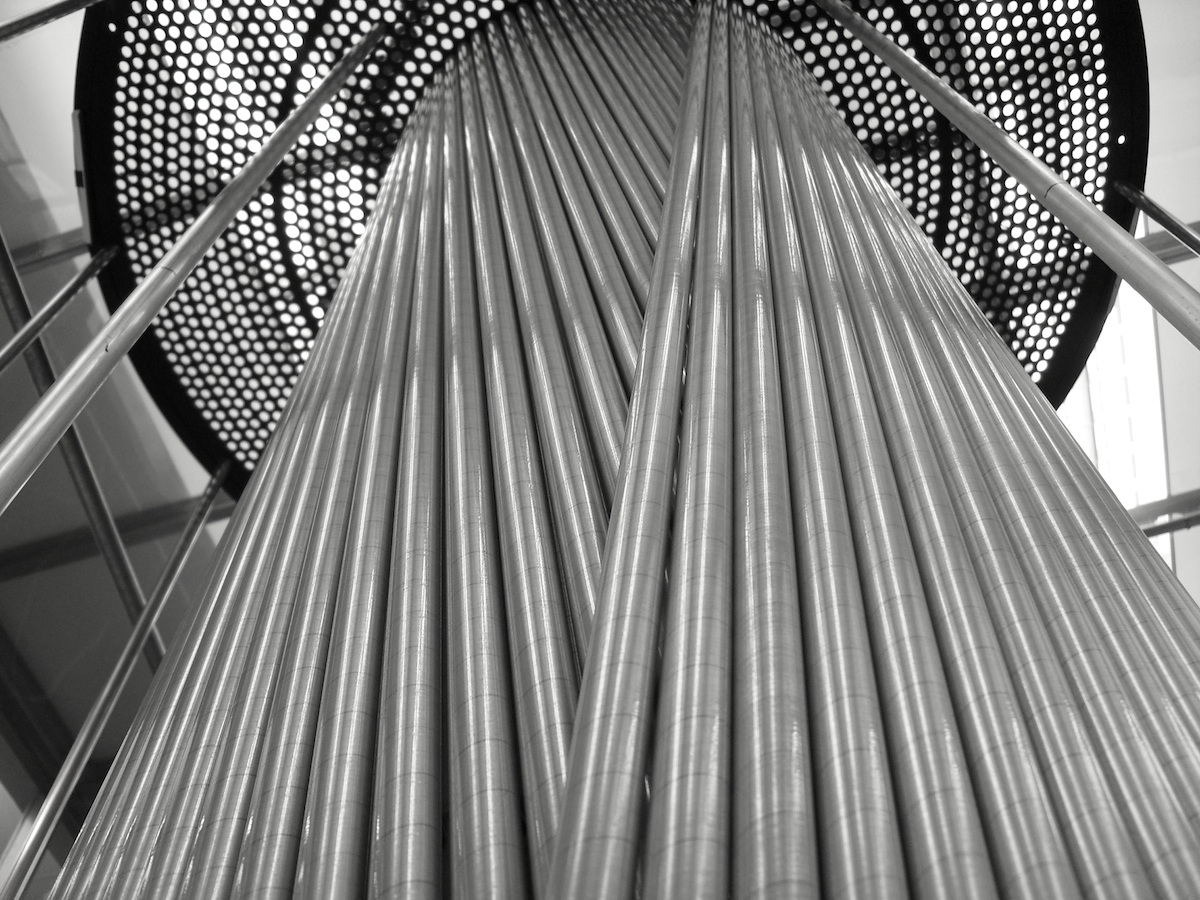
\includegraphics[width=0.7\textwidth]{figures/CDC_stereotubes.jpg}  
\caption{\label{fig:CDC_stereotubes}          
  The Central Drift Chamber during construction. A partially completed layer of stereo straw tubes is shown, surrounding a layer of straw tubes at the opposite stereo angle. Part of the carbon fiber endplate, two temporary tension rods and some of the 12 permanent support rods linking the two endplates can also be seen.}  
\end{center}
\end{figure}

The volume surrounding the straws is enclosed by an inner cylindrical wall of 0.5\,mm G10 fiberglass, an outer cylindrical wall of 1.6\,mm aluminum, and two circular endplates. 
The upstream endplate is made of aluminum, while the downstream endplate is made of carbon fiber. The endplates are connected by 12 aluminum support rods. 
Holes milled through the endplates support the ends of the straw tubes, which were glued into place using several small components per tube, described more fully in~\cite{GlueXCDCNIM}.  
These components also support the anode wires, which were installed with 30~g tension.
At the upstream end these components are made of aluminum and were glued in place using conductive epoxy\footnote{TIGA 920-H, www.loctite.com}. 
This provides a good electrical connection to the inside walls of the straw tubes, which are coated in aluminum.
The components at the downstream end are made of Noryl plastic\footnote{www.sabic.com} and were glued in place using conventional non-conductive epoxy\footnote{3M Scotch-Weld DP460NS, www.3m.com}.
The materials used for the downstream end were chosen to be as lightweight as feasible so as to minimize the energy loss of charged particles passing through them. 

At each end of the chamber there is a cylindrical gas plenum outside the endplate.  
The gas supply runs in 12 tubes through the volume surrounding the straws into the downstream plenum. 
There it enters the straws and flows through them into the upstream plenum. From the upstream plenum the gas flows into the volume surrounding the straws, and from there it exhausts to the outside, bubbling through small jars of mineral oil.
The gas mixture used is 50$\%$ argon and 50$\%$ carbon dioxide at atmospheric pressure. 
This gas mixture was chosen since its drift time characteristics provide good position resolution~\cite{VanHaarlem:2010yq}.
A small admixture (approximately 1$\%$) of isopropanol is used to prevent loss of performance due to aging\cite{KADYK1991436,VAVRA20031}. 
Five thermocouples are located in each plenum and used to monitor the temperature of the gas.
The downstream plenum is 2.54~cm deep, with a sidewall of ROHACELL\footnote{www.rohacell.com} and a final outer wall of aluminized Mylar film, and the upstream plenum is 3.18~cm deep, with a polycarbonate sidewall and a polycarbonate disc as its outer wall. 

The readout cables pass through the polycarbonate disc and the upstream plenum to reach the anode wires. 
They are connected in groups of 20 to 24 to transition boards which are mounted onto the polycarbonate disc and support the connectors for the high-voltage boards. 
Preamplifiers~\cite{hdnote2515} are mounted on the high-voltage boards. The aluminum endplate, outer cylindrical wall of the chamber, aluminum components connecting the straws to the aluminum endplate and the inside walls of the straws are all connected to a common electrical ground. 
The anode wires are held at +2.1~kV during normal operation. 


\subsection[Forward Drift Chamber]{Forward Drift Chamber
\label{sec:fdc} }

The Forward Drift Chamber (FDC) consists of 24 disk-shaped planar drift chambers of 1m-diameter.
They are grouped into four packages inside the bore of the spectrometer magnet.
Forward tracking requires good multi-track separation due to the
high particle density in the forward region.
This is achieved via additional cathode strips on both sides of the wire plane allowing for a  reconstruction of a space point on the track from each chamber. 
The FDC registers particles emitted into polar angles as low as $1^\circ$ and up to $10^\circ $
with all the chambers, while having partial coverage up to $20^\circ$.

One FDC chamber consists of a wire plane with cathode planes on either sides at a distance of $5$~mm from the wires (Fig.~\ref{FDC_OneCell}).
\begin{figure}[tbp]
\begin{center}
%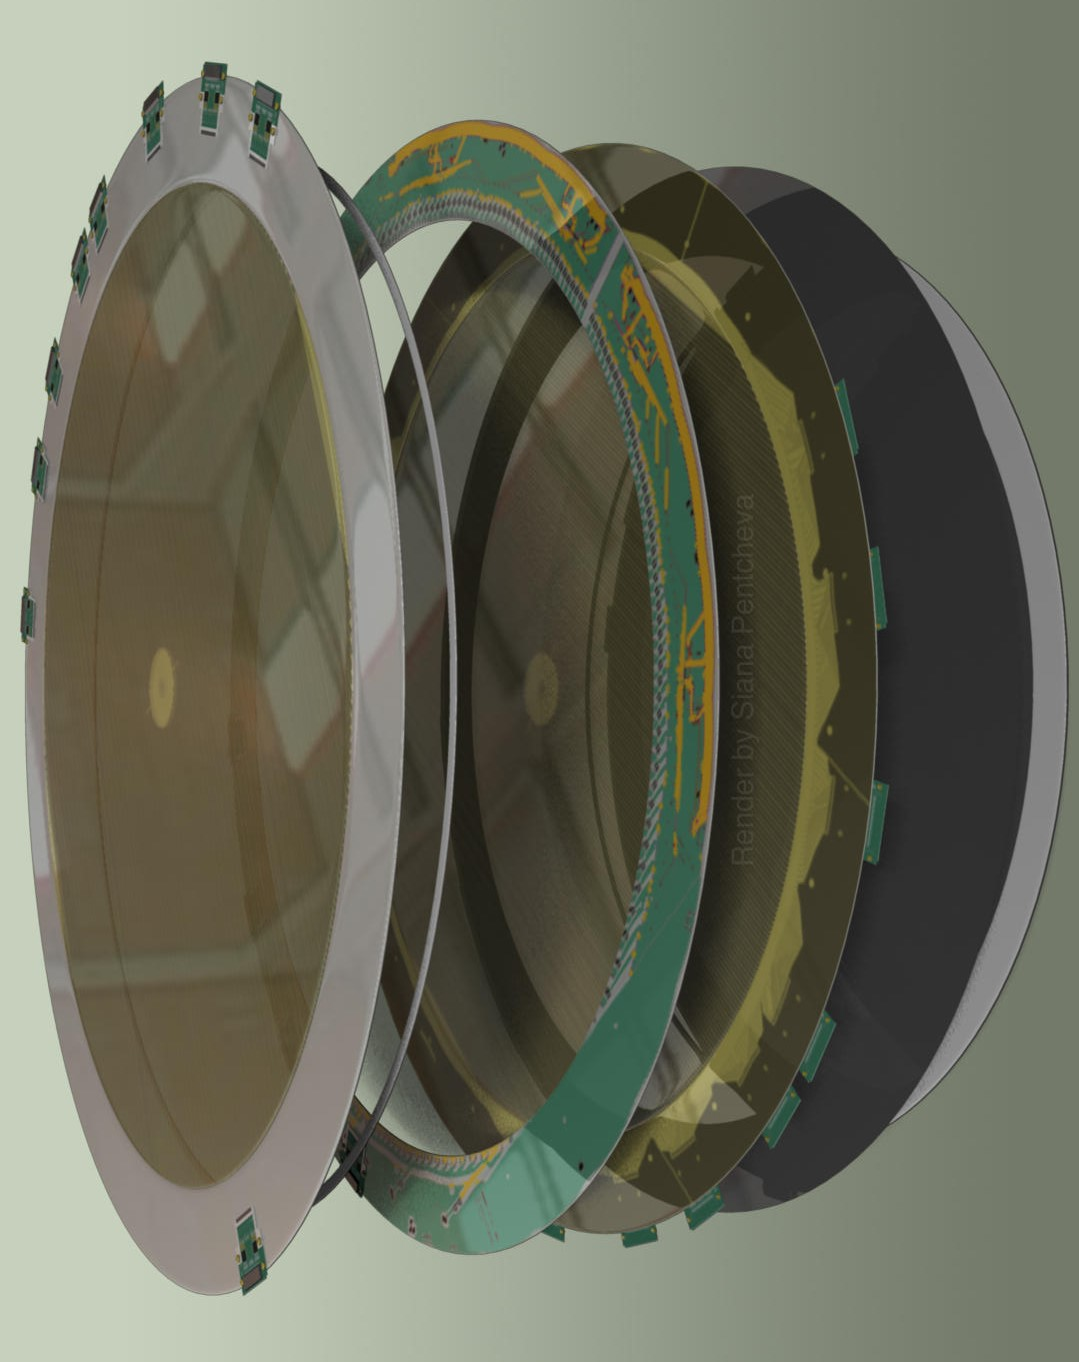
\includegraphics[width=0.75\textwidth]{figures/FDC_OneCell.jpg}  
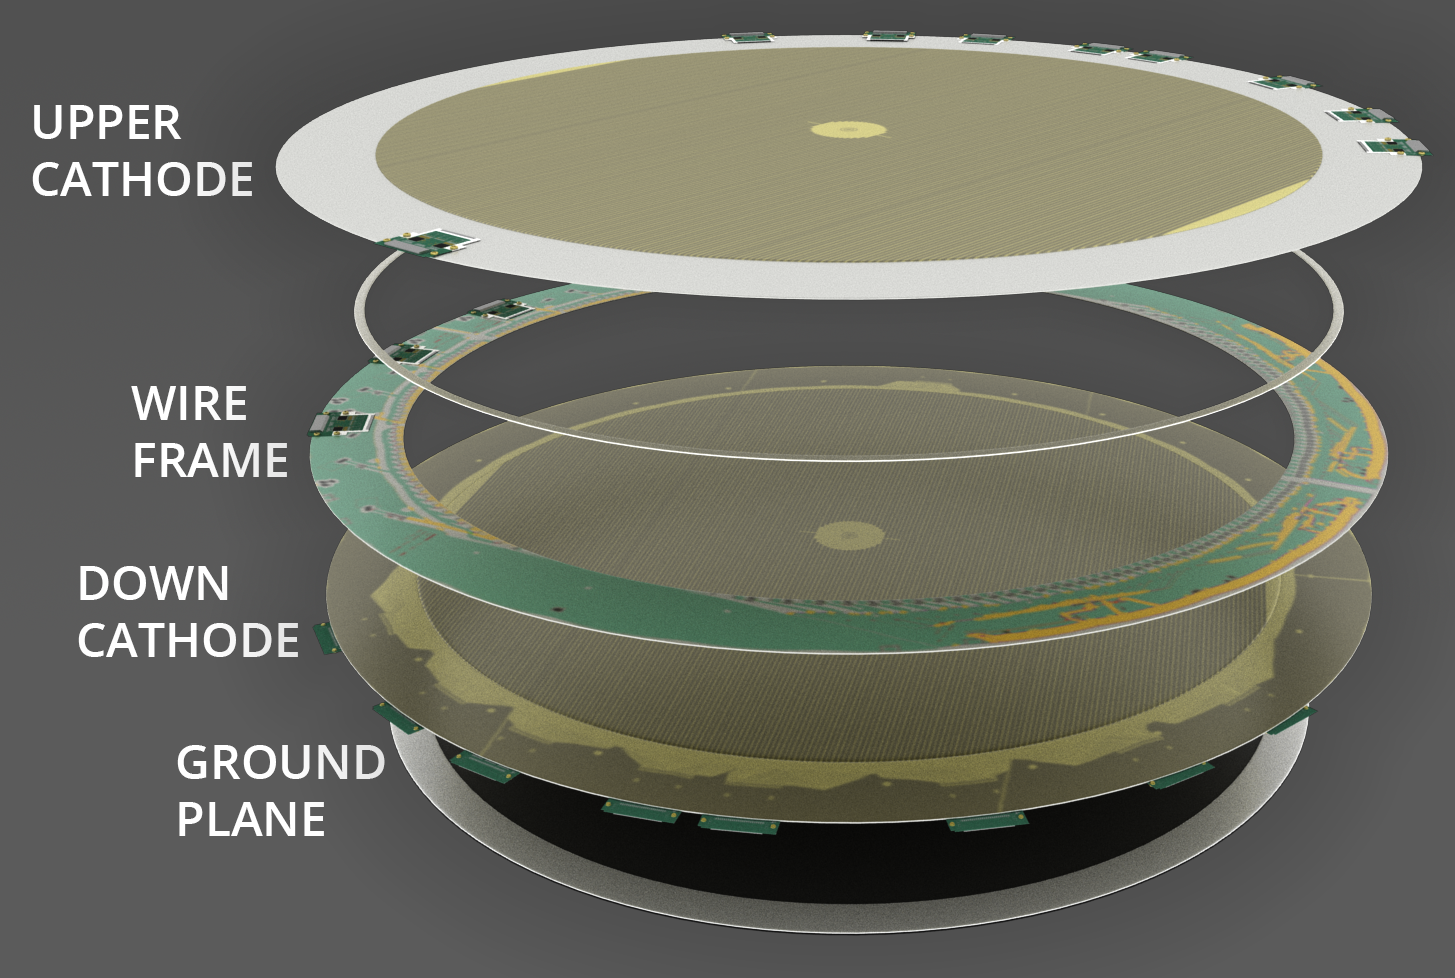
\includegraphics[width=0.95\textwidth]{figures/FDC_OneCell2.png} 
\caption{\label{FDC_OneCell}
Artistic view of one FDC chamber (from top to bottom): upstream cathode, wire frame, downstream cathode, ground plane that separates the chambers. The diameter of the active area is $1$~m.
}
\end{center}
\end{figure}
The frame that holds the wires is made out of Rohacell with a thin
G10 fiberglass skin in order to minimize the material and
allow low energy photons to be detected in the outer electromagnetic calorimeters.

The wire plane has sense ($20~\mu$m diameter) and field ($80$~$\mu$m) wires $5$~mm apart, forming a field cell of $10\times 10$~mm$^2$. 
To reduce the effects of the magnetic field 
a ``slow" gas mixture of $40\%$~Ar and $60\%$~CO$_2$ is used.
A positive high voltage of about $2.2$~kV is applied to the sense wires and a negative high voltage of $0.5$~kV to the field wires. 
The cathodes are made out of $2$-$\mu$m-thin $Cu$ strips on Kapton foil with a pitch of $5$~mm and are held at ground. The strips on the two cathodes are arranged at $30^\circ $ relative to each other and at angles of $75^\circ $ and $105^\circ $ angle with respect to the wires.

The six chambers of a package are separated by thin aluminized Mylar.
Each chamber is rotated relative to the previous one by $60^\circ $.
The total material of a package in the sensitive area corresponds to $0.43\%$ radiation lengths with about half of that in the area along the beam line that has no copper on the cathodes.
The sense wires in the inner area of $6-7.8$~cm diameter (depending on the distance of the package to the target) are increased in thickness from $20$~$\mu$m to $\sim 80$~$\mu$m which makes them insensitive to the high rates along the beam.
The distance between the first and last package is $169$~cm. 
All the chambers are supplied with gas in parallel. 
In total $2,304$ wires and $10,368$ strips are read using charge preamplifiers with $10$~ns peaking time with a gain of $0.77$~mV/fC for the wires and $2.6$~mV/fC for the strips.

\subsection{Electronics \label{sec:dcelectronics}}
The high voltage (HV) supply units used are CAEN A1550P\footnote{www.caen.it} with noise-reducing filter modules added to each crate chassis. 
The low voltage (LV) supplies are Wiener MPOD MPV8008\footnote{www.wiener-d.com}. 
The preamplifiers are a custom JLab design based on an ASIC~\cite{hdnote2515}
with 24 channels per board; they are charge-sensitive, and are capacitively coupled to the wires in the CDC and FDC and directly coupled to strips in the FDC. 

Pulse information from the CDC anode wires and FDC cathode strips are obtained and read out using 72-channel 125 MHz flash ADCs (FADCs) \cite{Visser2008,5873864}. These use Xilinx\footnote{www.xilinx.com} Spartan-6 FPGAs (XC6SLX25) for signal digitization and data processing with 12 bit resolution.
Each FADC receives signals from three preamplifiers. 
The signal cables from different regions of the drift chambers are distributed between the FADCs in order to share out the processing load as evenly as possible.  

The FADC firmware is activated by a signal from the GlueX trigger. It then computes the following for the next pulses observed above a given threshold within a given time window: pulse number, arrival time, pulse height, pulse integral, pedestal height immediately before the pulse, and a quality factor indicating if the arrival time is likely to be less accurate than usual. 
Signal filtering and interpolation are used to obtain the arrival time to the nearest 0.8~ns. 
The firmware performs these calculations both for the CDC and FDC alike, and uses different readout modes to provide the data with the precision required by the separate detectors. 
For example, the CDC electronics read out only one pulse but requires both pulse height and integral, while the FDC electronics read out up to four pulses and does not require a pulse integral.  

The FDC anode wires are read out using the GlueX F1TDC\cite{hdnote1021}. 

\subsection[Gas system]{Gas system \label{sec:gas}}
Both tracking chambers, the CDC and FDC, operate with the same gases, argon and CO$_{2}$. Since the relative mixture of
the two gases are slightly different for the two tracking chambers the gas system has two separate but identical mixing stations. There is one gas supply of argon and CO$_{2}$ for both mixing stations. A limiting opening in the supply
lines provides over-pressure protection to the gas system and filters in the gas lines provide protection against potential
pollution of the gas from the supply. Both gases are mixed together using mass flow controllers (MFCs) that can be 
configured
to provide the desired mixing ratio of argon and CO$_{2}$.  The MFCs and their control electronics are from
BROOKS Instruments.\footnote{BROOKS Instruments, https://www.brooksinstrument.com/en/products/mass-flow-controllers.}

The mixed gas is filled into storage tanks, one for the CDC and another for the FDC. Their pressures are
regulated by controlling the operation of the MFCs with a logic circuit based on an Allen-Bradley ControlLogix system\footnote{Allen-Bradley, https://ab.rockwellautomation.com/}
 (these are used throughout the experimental hall) that keeps
the pressure in the tank between 10 and 12~psi. The tank serves as a reservoir and a buffer.
A safety relief valve on each tank
provides additional protection against over-pressure. While the input pressure to the MFC is at 40~psi the pressure after
the MFC is designed to be always less than 14~psi above atmospheric pressure. After the mixing tank there is a provision
built into the system to let the gas pass through an alcohol bath to add a small amount to the gas mixture.
This small admixture of alcohol protects the wire chambers from aging effects caused by radiation exposure from the beam.
This part of the gas system is located above ground in a separate gas shed before the gas mixture is transported
to the experimental hall via polyethylene pipes.

Additional MFCs in the hall allow the exact amount of gas provided to the chambers to be specified. There is one for the CDC and another 
four for the individual FDC packages. The CDC is operated with a flow of 1.0~l/m while each FDC package is operated with
a flow of 0.1~l/m. To protect the chambers from over-pressure there is a bypass line at the input to the detectors that
is open to the atmosphere after a bubbler containing of mineral oil. The height of the oil level determines the maximum possible gas pressure at
the input to the chambers. There is a second bubbler at the output to protect against possible air back-flow into
the chamber. The height of its oil above the exhaust line determines the operating pressure inside the chambers.

Valves are mounted at many locations in the gas system to monitor various pressures with a single pressure sensor. The pressures of all six FDC chambers are monitored, as well as the CDC gas at the input, downstream gas plenum and the exhaust. 
A valve in the exhaust line can be used to divert some gas from the chamber to an oxygen sensor. Trace quantities of oxygen will reduce the gas gain and reduce tracking efficiency. The oxygen levels in the chamber are below 100~ppm.

\subsection{Calibration, performance and monitoring \label{sec:dccalib}}
Time calibrations for the drift chambers are used to remove the time offset due to the electronics, so that after calibration the earliest possible arrival time of the pulse signals is at 0~ns. These offsets and the function parameters used to describe the relationship between the pulse arrival time and the closest distance between the track and the anode wire are obtained for each session of data taking. 

The CDC measures the $dE/dx$ of tracks over a wide range of polar angles, including recoiling target protons as well as more forward-going tracks. Gain calibrations are made to ensure that the $dE/dx$ is consistent between tracking paths through different straws and stable over time. 
The procedure entails matching the position of the minimum ionizing peak for each of the 3522 straws, and then matching the $dE/dx$ at 1.5~GeV/c to the calculated value of 2.0~ keV/cm. This takes place during the early stages of data analysis. Gain calibration for the individual wires is performed each time the HV is switched on and whenever any electronics modules are replaced. Gain calibration for the chamber as a whole is performed for each session of data taking; these are limited to two hours as the gain is very sensitive to the atmospheric pressure. Position calibrations were necessary to describe the small deflection of the straw tubes midway along their length; these were performed in 2016 and repeated in 2017, with no significant difference found between the two sets of results.  Position resolution from the CDC is of the order of 130~$\mu$m and its detection efficiency per straw is over 98\% for tracks up to 4~mm from the wire. The efficiency decreases as the distance between the track and the wire increases, but the close-packing arrangement of the straw tubes and the large number of straws traversed by each track compensate for this. 

For the FDC system, an internal per-chamber calibration process is first performed to optimize the track position accuracy.  
In the FDC the avalanche created around the wire is seen in three projections: on the two cathodes and on the wires.
The drift time information from the wires is used to reconstruct the hit position perpendicular to the wire.
The strip charges from the two cathodes are used to reconstruct the avalanche position along the wire. 
The same strip information can be used to reconstruct the avalanche position perpendicular to the wire,  which, due to the proximity of the avalanche to the wire, is practically the wire position, as illustrated in Fig~\ref{FDC_wires_from_strips}.
\begin{figure}[tbp]
\begin{center}
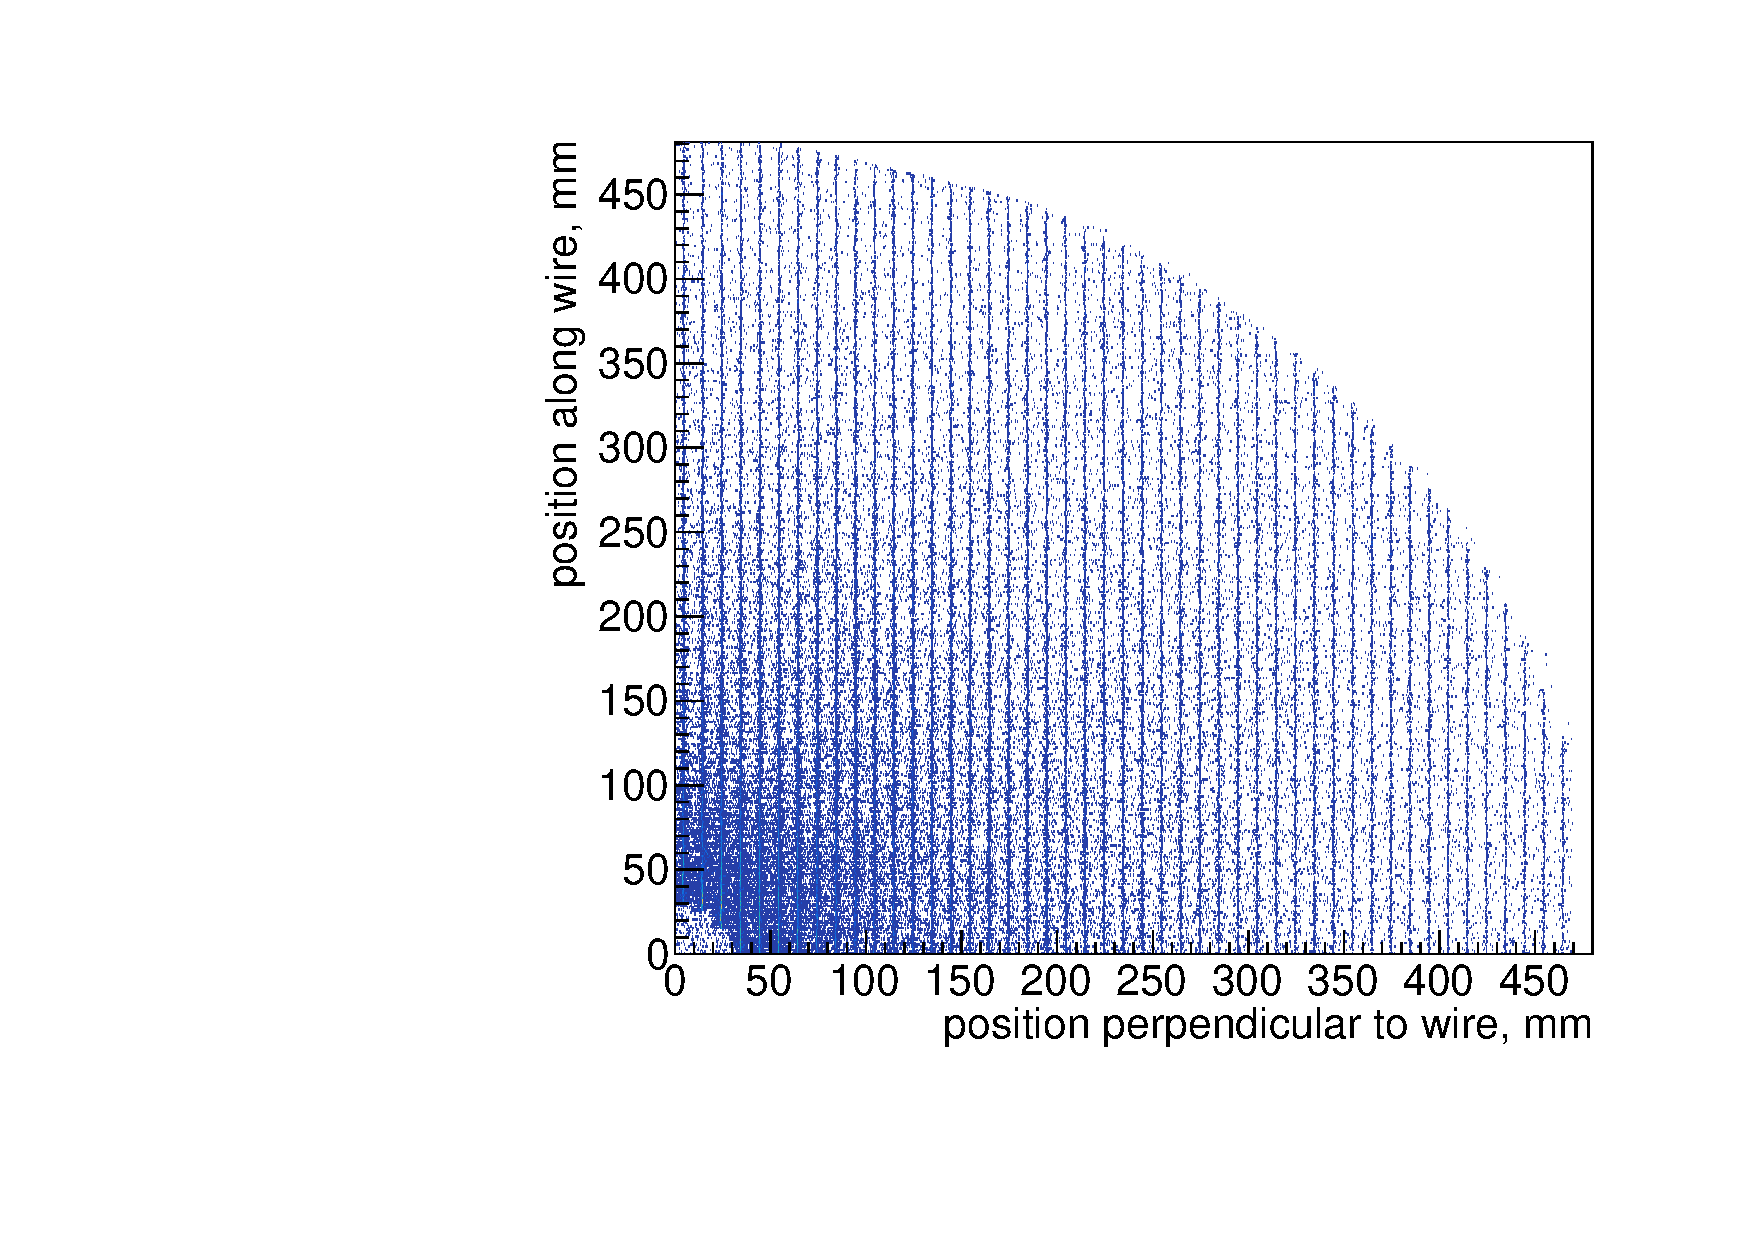
\includegraphics[width=0.95\textwidth]{figures/FDC_wires_from_strips1.pdf}  
\caption{\label{FDC_wires_from_strips} Wire (avalanche) positions reconstructed from the strip information on the two cathodes in one FDC chamber. Shown is only one quarter of the chamber.
}   
\end{center}  
\end{figure}
This is used to align the strips on the two cathodes with respect to the wires. 
At the same time the residuals of the reconstructed wire positions are an estimate of the strip resolution.
The resolutions of the detector were reported earlier \cite{FDC_NIM}. 
The strip resolution along the wires, estimated from the wire position reconstruction, varies between $180$ and $80$~$\mu$m, depending on the total charge induced on the strips. The drift distance is reconstructed from the drift time with a resolution between $240$ and $140$~$\mu$m
depending on the distance of the hit to the wire in the $0.5-4.5$~mm range.  

Position offsets and package rotations were determined for both drift chamber systems, first independently, and then together, using the alignment software MILLEPEDE\cite{millepede} in a process described in \cite{GlueXCDCNIM} and in \cite{MikeStaib_thesis}.

Online monitoring software enables the shift-takers to check that the number of channels recording data, the distribution of signal arrival times and the  $dE/dx$ distribution are as expected. 


%\subsection{Summary \label{sec:dcsummary}}
 
 

\section[Performance of the charged particle tracking system (Simon)]{Performance of the charged particle tracking system}
\subsection{Track reconstruction}
\subsection{Tracking efficiency}
\subsection{Momentum resolution}
\subsection{Vertex resolution}
\section[Electromagnetic calorimeters (Elton/Colin)] {Electromagnetic calorimeters \label{sec:calorimeters}}
\subsection[Barrel calorimeter ]{Barrel calorimeter \label{sec:bcal}}
The barrel calorimeter (BCAL) detects photon showers with energies between 0.05 GeV and several GeV, $11^{\circ}$--$126^{\circ}$ in polar angle, and $0^{\circ}$--$360^{\circ}$ in azimuthal angle. Details of the design, construction and performance of the BCAL can be found in Ref.\cite{BEATTIE201824}. The containment of showers depends on the angle of particle incidence, with a thickness of $15.3$ radiation lengths for particles entering normal to the calorimeter face and reaching up to 67 radiation lengths at $14^{\circ}$. Geometrically, the BCAL consists of 48 optically isolated modules each with a trapezoidal cross section, forming a  390~cm-long cylindrical shell having inner and outer radii of 65~cm and 90~cm, respectively. The fibers run parallel to the cylindrical axis of the detector.  Details of the end of the calorimeter with light guides, light sensors and electronics are shown in  Fig.\,\ref{fig:bcal:bcal_assemblies}.

\begin{figure}[http]\centering
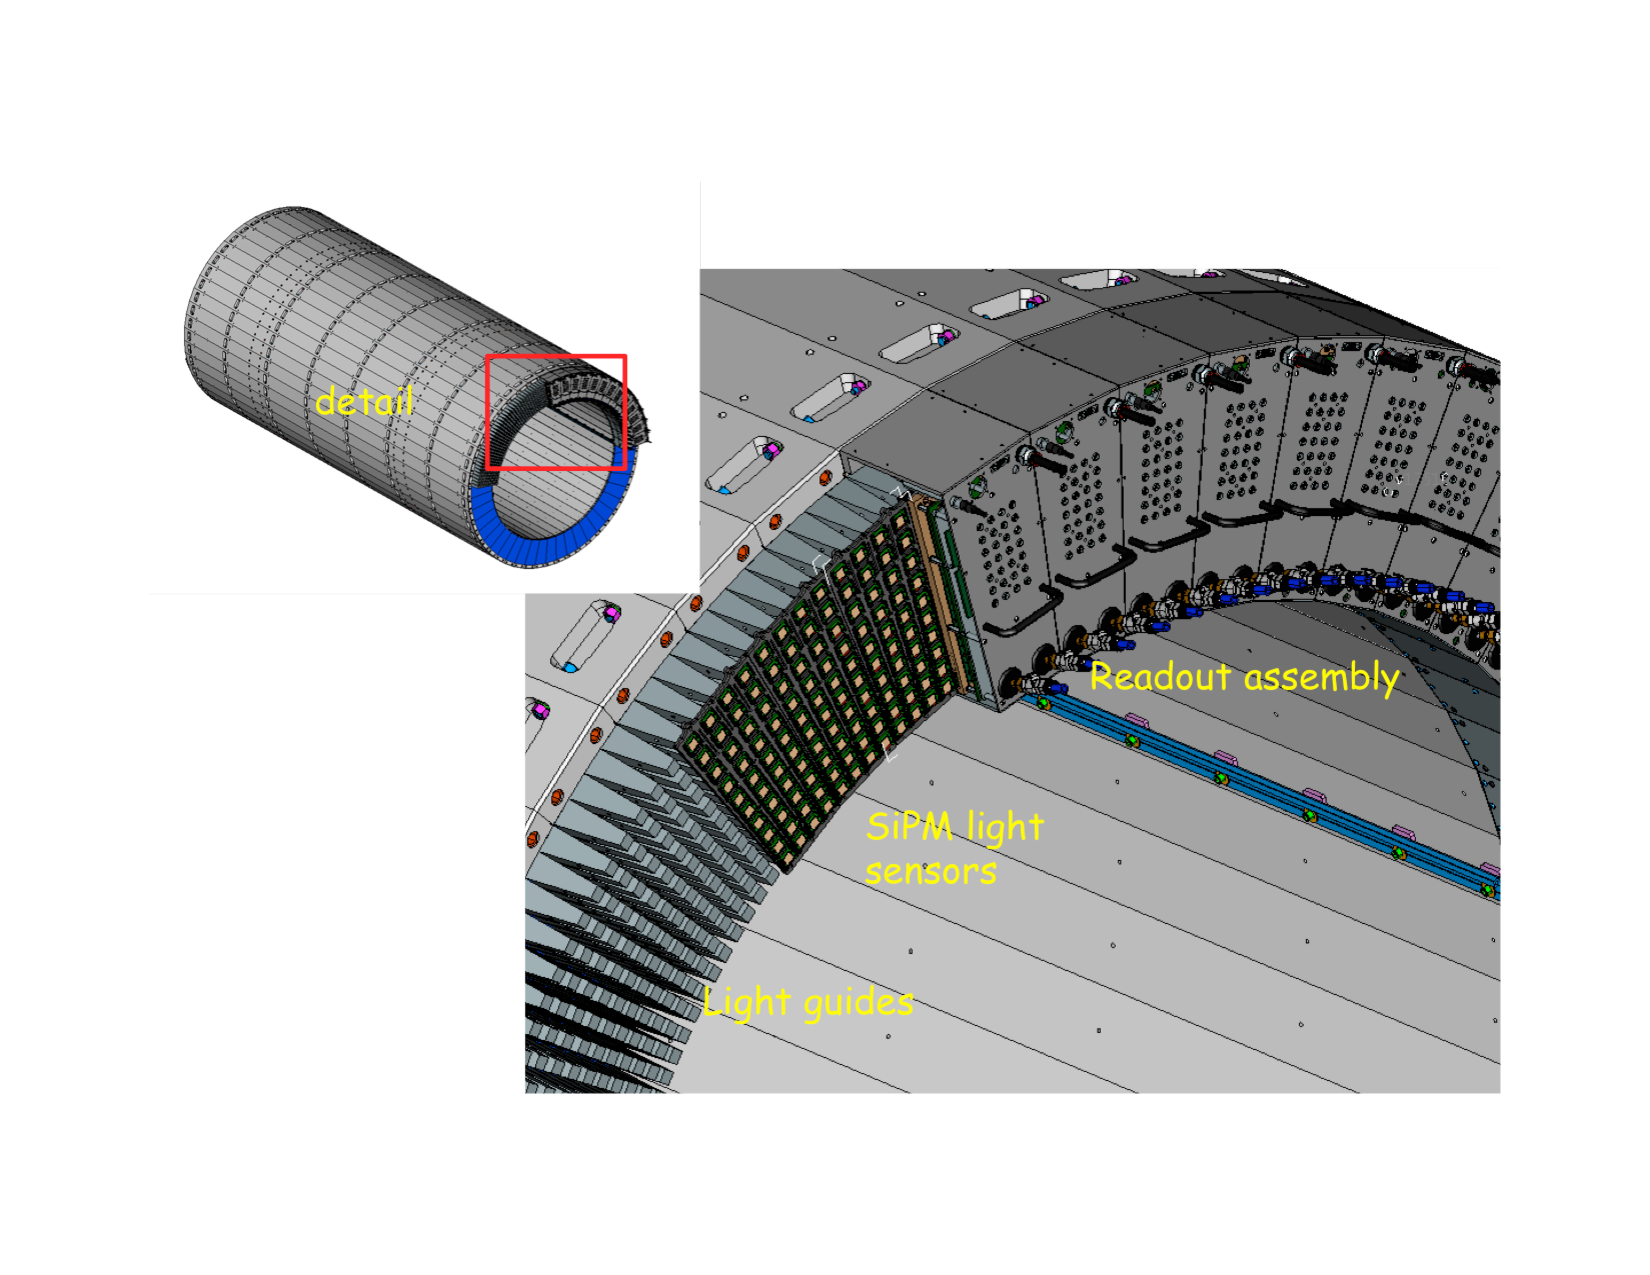
\includegraphics[scale=0.4]{figures/bcal_assemblies.pdf}
\caption{\label{fig:bcal:bcal_assemblies}
   Three-dimensional rendition of the light guides mounted at the end of the 
   BCAL, as well as the readout assemblies mounted over them. The 
   readout assemblies contain the 
   SiPMs and their electronics.  (Color online)
  }
\end{figure}
The BCAL is constructed as a lead and  scintillating-fiber matrix
and read out with silicon photomultiplier (SiPM) arrays. The matrix consists of 0.5 mm-thick grooved lead sheets and 1.0 mm-diameter Kuraray SCSF-78MJ multi-clad fibers.
Each module has approximately 185 layers and 15,000 fibers.
Particles impinge on the detector over a wide range of angles, from normal incidence at 90 degrees down to 11.5 degrees, which defines a geometry that is fairly unique among calorimeters. 

The light is collected via small light guides at each end of the module and transported to the SiPMs, which were chosen due to their insensitivity to magnetic fields. 
The light sensors are Hamamatsu S12045(X) Multi-Pixel Photon Counter (MPPC) arrays \footnote{Hamamatsu Corporation, Bridgewater, NJ 08807, USA \\ (\url{http://sales.hamamatsu.com/en/home.php)}.}, 
which are $4\times4$ arrays of $3\times3$ mm$^2$ tiles \cite{hdnote2913}.
The SiPMs were tested extensively before acceptance
\cite{Barbosa2012100,Qiang2013234,soto,Soto201489,doi:10.1063/1.4955340}.
Four thousand units were purchased and 3840 are installed in the detector.
The gain of the SiPM depends on the voltage above the breakdown voltage, which is about 70~V. We operate them at 1.4 V over the breakdown voltage, which was selected to reduce the effect of readout thresholds. Even at this relatively high over-bias, the noise level is dominated by fluctuations in the electronics baseline and not by single-pixel noise. In order to keep a constant gain, 
we maintained the temperature within practical limits ($\pm$ 2$^\circ$C) 
using a chilled water system and then stabilized the gain 
using a custom circuit that adjusted the bias voltage based on the measured temperature. Two stages of preamplifiers and summing electronics are attached to the sensors. In order to reduce the number of signals that are digitized, circuits sum the outputs of the preamplifiers in groups of radial columns, with coarser granularity away from the target. The layer closest to the target consists of a single SiPM. On the end of each module, forty SiPMs generate sixteen signals that are delivered to flash ADCs (FADCs) and twelve signals that are discriminated and then recorded with pipeline TDCs. The FADCs and TDCs are conveniently located on the floor of the experimental hall in VXS crates.
  
  
\begin{figure}[tbp]\centering
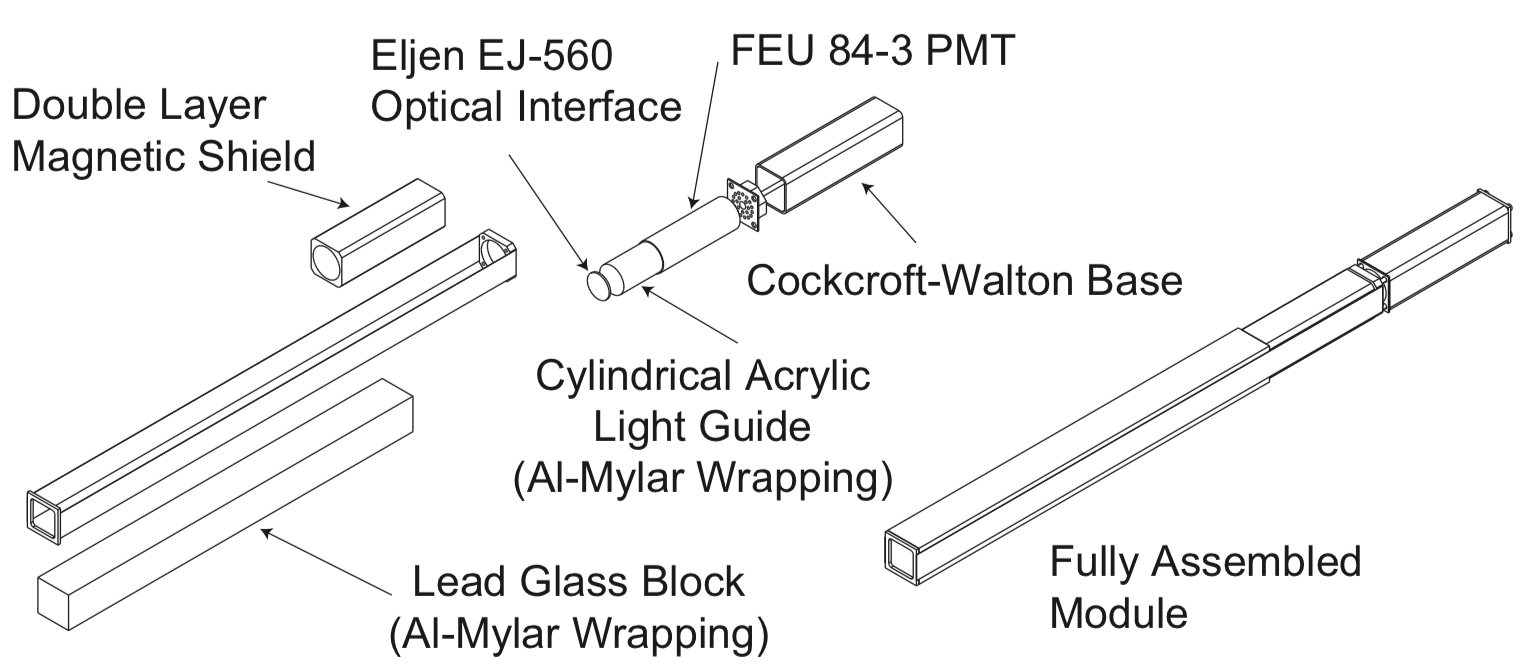
\includegraphics[height=5cm]{figures/FCAL_single_module}
\caption{\label{fig:fcal:FCAL_single_module}
    Expanded view of a single FCAL module.
  }
\end{figure} 
\subsection{Forward calorimeter \label{sec:fcal}}
The forward calorimeter (FCAL) detects photon showers with energies ranging from 0.1 GeV to several GeV between $1^{\circ}$--$11^{\circ}$. The FCAL is located 5.6\,m downstream from the center of the GlueX target and consists of 2800 lead glass blocks stacked in a circular array that has a diameter of 2.4\,m.  The lead glass blocks were equivalent to type F8 manufactured by the Lytkarino Optical Glass Factory,\footnote{http://lzos.ru .} and each have transverse dimensions of $4\times4$ cm$^2$ and are 45 cm long. The lead-glass blocks and most of the PMTs are the same as those used in previous experiments, E852 at Brookhaven National Laboratory 
\cite{CRITTENDEN1997377} and the RadPhi Experiment at JLab \cite{JONES2007384}. The glass was annealed by heat treatment prior to installation in GlueX. 
The light collection from the lead-glass block into the photomultiplier tube (PMT) is accomplished via an acrylic cylindrical light guide glued to the PMT. An Eljen EJ-560 optical interface ``cookie'' is used to connect the guide to the lead glass block. 
The sensors are FEU 84-3 photomultipliers with Cockcroft-Walton bases, consuming 0.2 W of power.  The design of the PMT base is similar to that noted in Ref.~\cite{Brunner:1998fh}
and eliminates the need for a 2400-channel high-voltage power system. The light guide recesses the magnetically sensitive photocathode of the PMT inside a dual layer of soft iron and mu-metal that attenuates the stray field of the GlueX solenoid of up to 200 G. The bases communicate with a controller utilizing the CAN protocol \cite{}, with 100 bases on each of 28 different CAN busses.  The communication allows continuous monitoring of various voltages, temperature, and current draw of the base.
A schematic of a single FCAL module is shown in 
Fig.\,\ref{fig:fcal:FCAL_single_module} and more details may be found in Ref.\,\cite{MORIYA201360}.

\subsection{Electronics \label{sec:calelectronics}}
Custom readout electronics are mounted in standard VXS crates and include 
JLab 12-bit 250~MHz FADCs \cite{hdnote1022}, discriminators \cite{hdnote2511} and F1 Time-to-Digital Converters (TDCs) \cite{hdnote1021}. The maximum input scale of the FADCs (4095 counts) is set to 2\,V.
% (mrs: I thought the ring buffer in the FADC was several microseconds long -- what is the 100 sample segemenation that is referred to in the next sentence?)
The FADCs sample each calorimeter channel every 4\,ns and generate raw waveforms consisting of 100 samples 
 (400\,ns), which are available for further processing by the firmware upon a trigger signal if there is a threshold crossing. The firmware computes several derived features of the pulse: pedestal, peak value, integral over a selected window, and
 time of the half-way point on the leading edge. At most one pulse is extracted from each readout window. These pulse features constitute the raw data that is read out from the FADC. 
 Optionally, the full waveforms can be read out for diagnostic purposes
 and to check the firmware output against the offline emulation of the parameter extraction. We record full waveforms in less than about 1\% of the production runs. 
 Pulses are identified by the first sample that exceeds a threshold, 
 currently set to 5 (8) counts above the average pedestal for the BCAL (FCAL).  The integral is determined using a fixed number of samples relative to the threshold crossing, 
 which was determined by maximizing the ratio of signal to pedestal noise. 
 The integration window begins one sample before the threshold time and extends to 26 (15) samples after the threshold time for the BCAL (FCAL).
 Typical pedestal widths are $\sigma\sim$1.2-1.3 (0.8) counts for the BCAL (FCAL).  For the BCAL, the pedestals are determined for each channel event-by-event, appropriately scaled, and then subtracted from the peak and integral to obtain signals proportional to the energy deposited in the calorimeter, while for the FCAL, the average pedestal over a run period is determined offline for each channel and its contribution to the pulse integral is subtracted when the data are reconstructed.%See Fig.\,\ref{fig:Plot_waveform10}.
 The algorithm that determines the time of the pulse is pulse-height independent and therefore no time-walk correction is required for the FADC times~\cite{Bennett:2010nf}.

The outputs of the three inner layers of the BCAL cells are also connected leading-edge discriminators, which feed the JLab F1 TDCs. 
 The discriminator thresholds are typically set to about 35 mV, but are adjusted
 channel by channel.  The pulse times are recorded relative to the trigger in a 12-bit word. Multiple hits, up to eight, may be recorded per channel per event, but are culled at a later time by comparison to FADC times. The nominal least count is configured to 58\,ps.


\subsection[Calibration and monitoring]{Calibration and monitoring \label{sec:calcalib}}
The relative gains of the calorimeters are monitored using a modular LED-driver system \cite{Anassontzis201441}. The control system is the same for both calorimeters, but the arrangement of LEDs is tailored to the geometry of each detector. In the BCAL, there is one LED inserted into each light guide, which can be used to monitor each individual SiPM and its partner at the far end of the module.
Due to geometry the illumination varies considerably from channel to channel. 
The average stability of the detector over a period of ten days is better than 1\% and the fractional root-mean-square (RMS) deviations of the mean for each SiPM during a single data from the average over the run period is typically less than 2\%.

For the FCAL, we installed four plexiglass panes, each covering the upstream end of one quadrant of the FCAL. Each pane is illuminated by forty LEDs, ten violet, ten blue and twenty green. In addtion to monitoring the stability of the readout, the different colors are used to study the wavelength dependence of the transmission of light though the the lead glass blocks.  In particular, radiation damage to lead glass inhibits transmission at the blue end of the spectrum and tends to turn glass a brownish color~\cite{Schaefer:2011gw}.  Throughout a several-month run, in the blocks closest to the beam line, the the PMT response to violet LED degrades by about 10\% while the response to the green LED is unchanged, characteristic of radiation damage.  Such damage is only evident in the first two layers of blocks around 12~cm$\times$12~cm opening for the beam to pass through.


\subsection{Performance \label{sec:calperformance}}
The performance of the calorimeter is summarized by its ability to measure the energy, position and timing of electromagnetic showers. 
The energy resolution of the BCAL was extracted from the measured $\pi^0$ and
$\eta$ mass distributions, which yielded consistent results. To study the $\eta$ mass resolution, we selected events
using kinematic fits to $\gamma p \rightarrow p \pi^+ \pi^- \gamma \gamma$. 
This reaction provides a fairly clean sample of $\eta$'s where both photons are recorded in the BCAL. The charged tracks were used to determine the event vertex needed to reconstruct the two-photon invariant mass.  The MC simulation 
generated $\gamma p \rightarrow p \pi^+ \pi^- \eta$ events, with $\eta\rightarrow \gamma\gamma$, where the kinematics were chosen to approximate the experimental distributions. The fitted Gaussian widths are shown in Fig.\,\ref{fig:bcal:eta_resolution}a as a function of the photon energy, both for data and simulation. 
The single-photon energy resolution can be determined from the $\eta$ width by neglecting contributions from the opening angle.
This is shown in Fig.\,\ref{fig:bcal:eta_resolution}b, where one can see that the resolution extracted from the data is only slightly above the MC. If we average the response over the $\pi^0$ and $\eta$ spectra we find 
$\sigma_E/E$=5.2\%/$\sqrt{E(\rm{GeV})} \oplus$ 3.6\%. The large constant term is artificially large because of the averaging over angles; at a single angle in the forward direction, the constant term is less than 1.7\%.

The position resolution ($\sim$\,2.5 cm) is determined by the timing resolution of the system, which was determined to be $\sigma$\,=\,150\,ps at 1\,GeV.
 


\begin{figure}[tbh]\centering
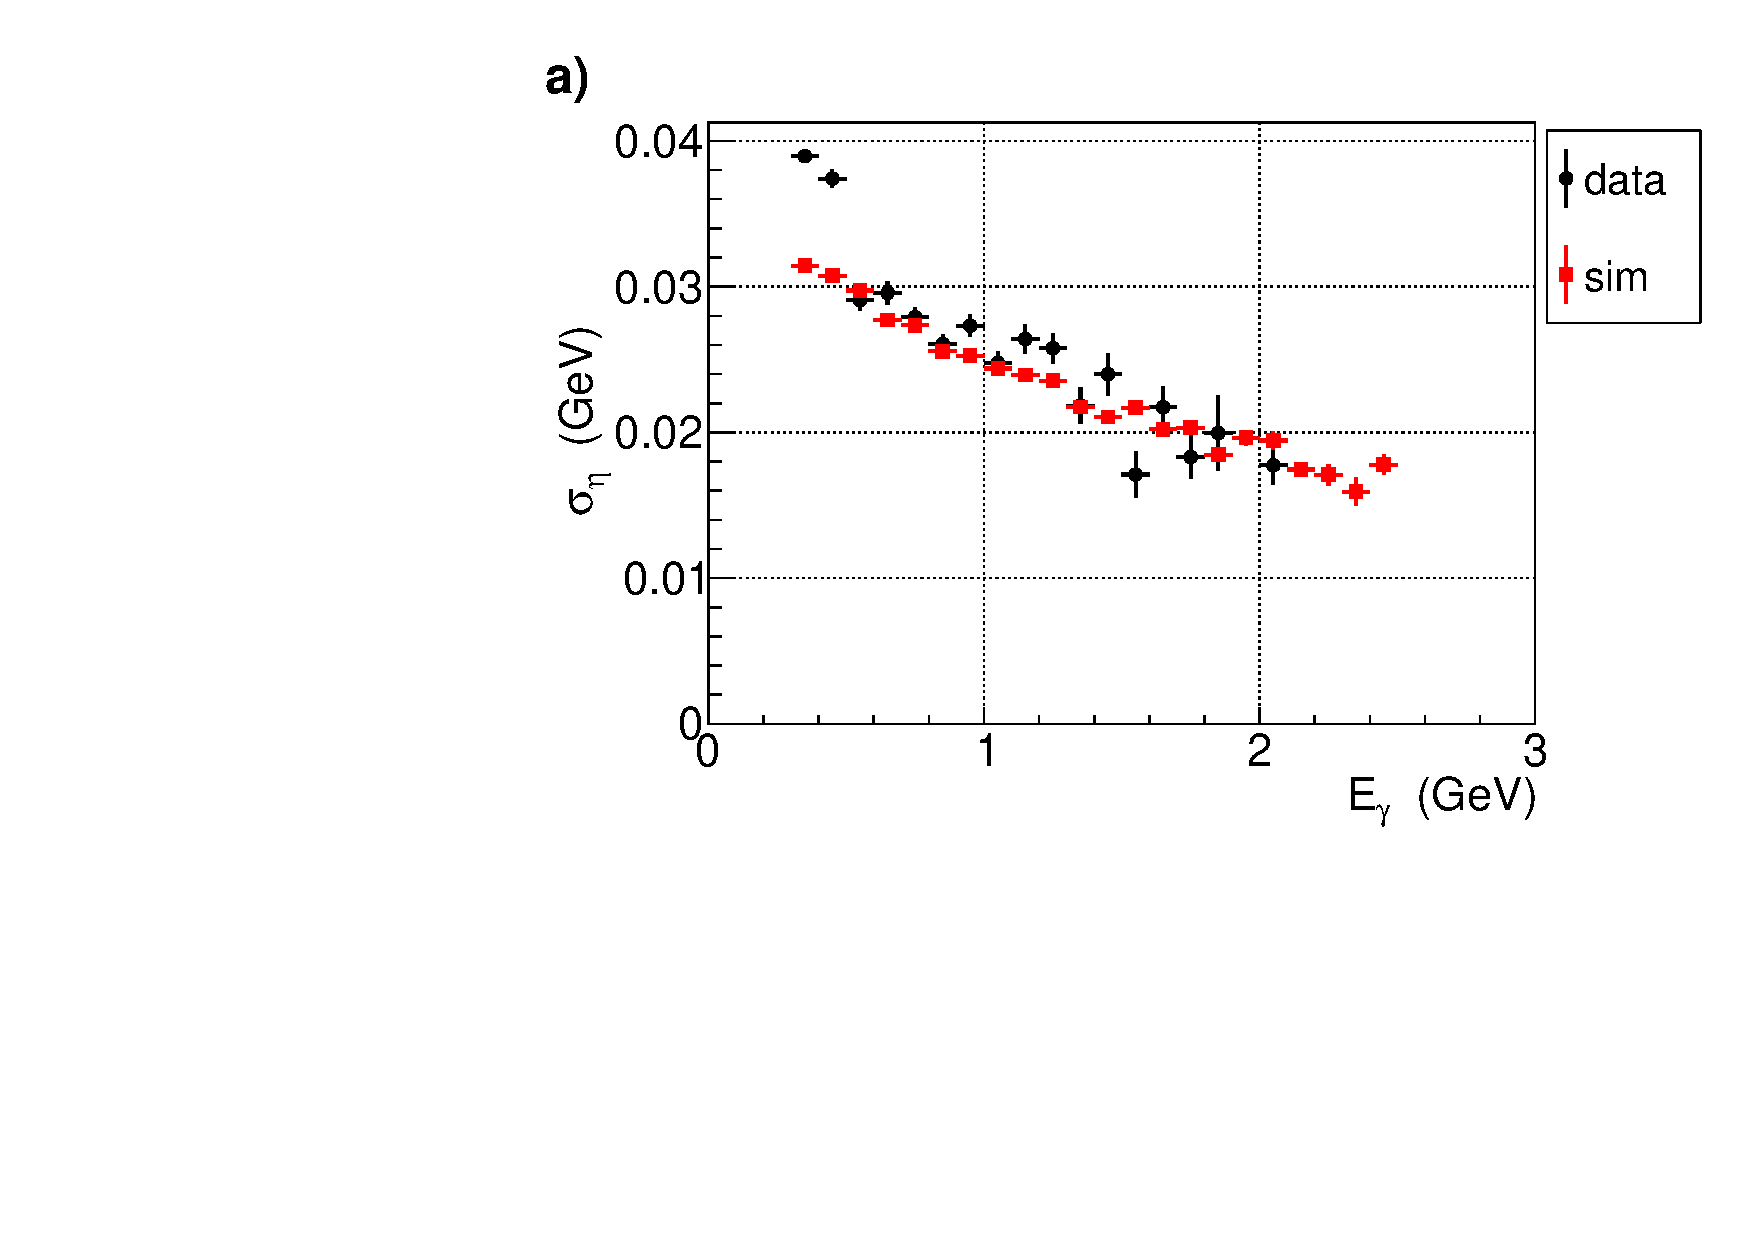
\includegraphics[width=0.45\textwidth]{figures/mcsmear50_37_gPsym100_etamass_sigma.pdf}   
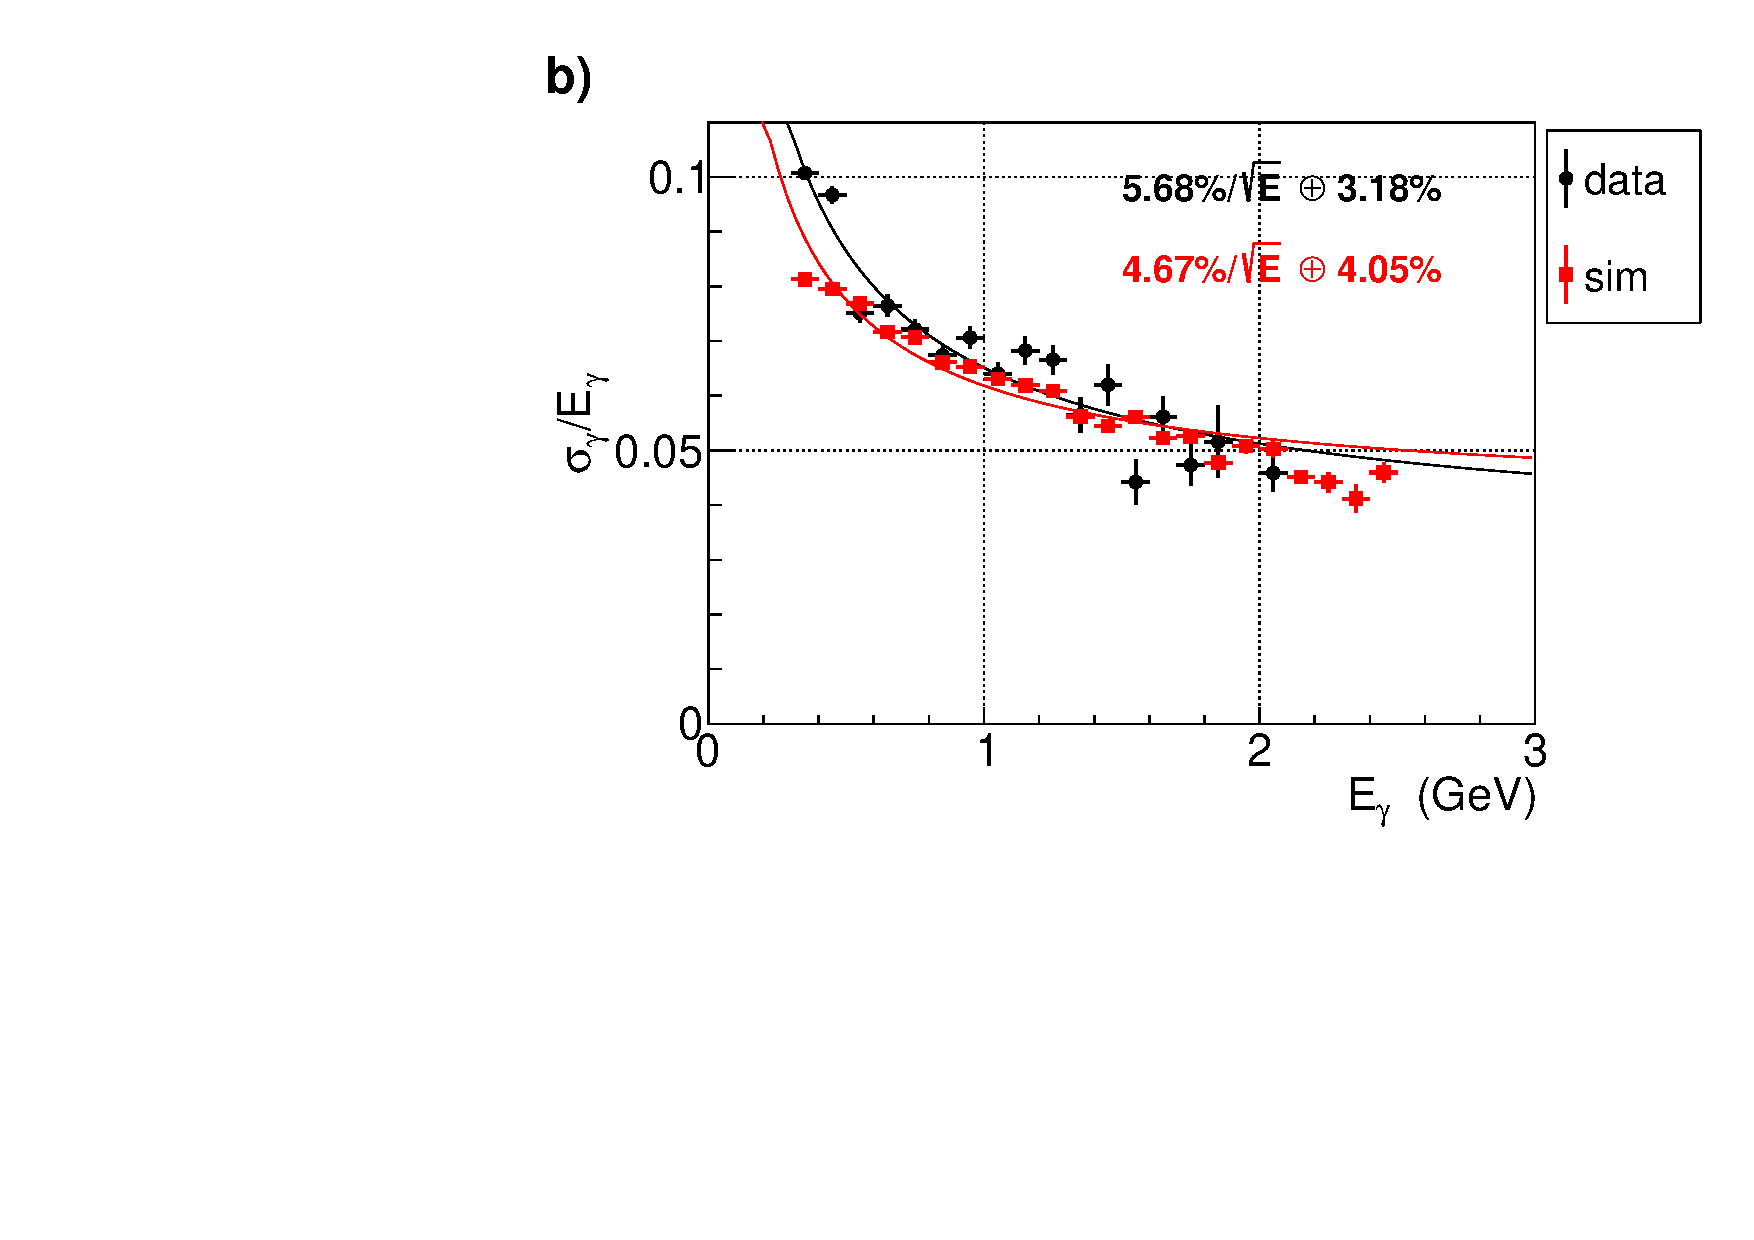
\includegraphics[width=0.45\textwidth]{figures/mcsmear50_37_gPsym100_E_sigma.pdf}
\caption{\label{fig:bcal:eta_resolution}
a)  Measured and simulated  $\eta$ width as a function of energy for symmetric decays, where both photons are required to be within 0.1 GeV of each other. 
b) The energy resolution of single photons calculated under the assumption that only the energy resolution contributes to the $\eta$ width. The curves are fits based on  Eq.\,\ref{eq:resolutionfit}.
(Color online)
 }
\end{figure}    






\subsection{Summary \label{sec:calsummary}}
\clearpage    % avoid formatting problems with empty sections
\section[Scintillation detectors (Mark I./Beni)]{Scintillation detectors \label{sec:scintillators}}
\subsection{Start counter \label{sec:st}}

The Start Counter (ST) detector, shown in Fig.~\ref{fig:st-overview-drawing}
surrounds the target
region and covers about 90\% of the solid angle for particles
originating from the center of the target. It is designed to operate
at tagged photon beam intensities of up to $10^8$ photons per second
in the coherent peak. It has a high degree of segmentation to limit
the the per-paddle rates. The time resolution is less than 350 ps
RMS. The Start Counter provides a timing signal that is releatively
independent of particle type and trajectory (because of its proximity
to the target), can provide particle identification via $dE/dx$, and
can be used in the Level 1 trigger.

\begin{figure}[!htb]
\centering
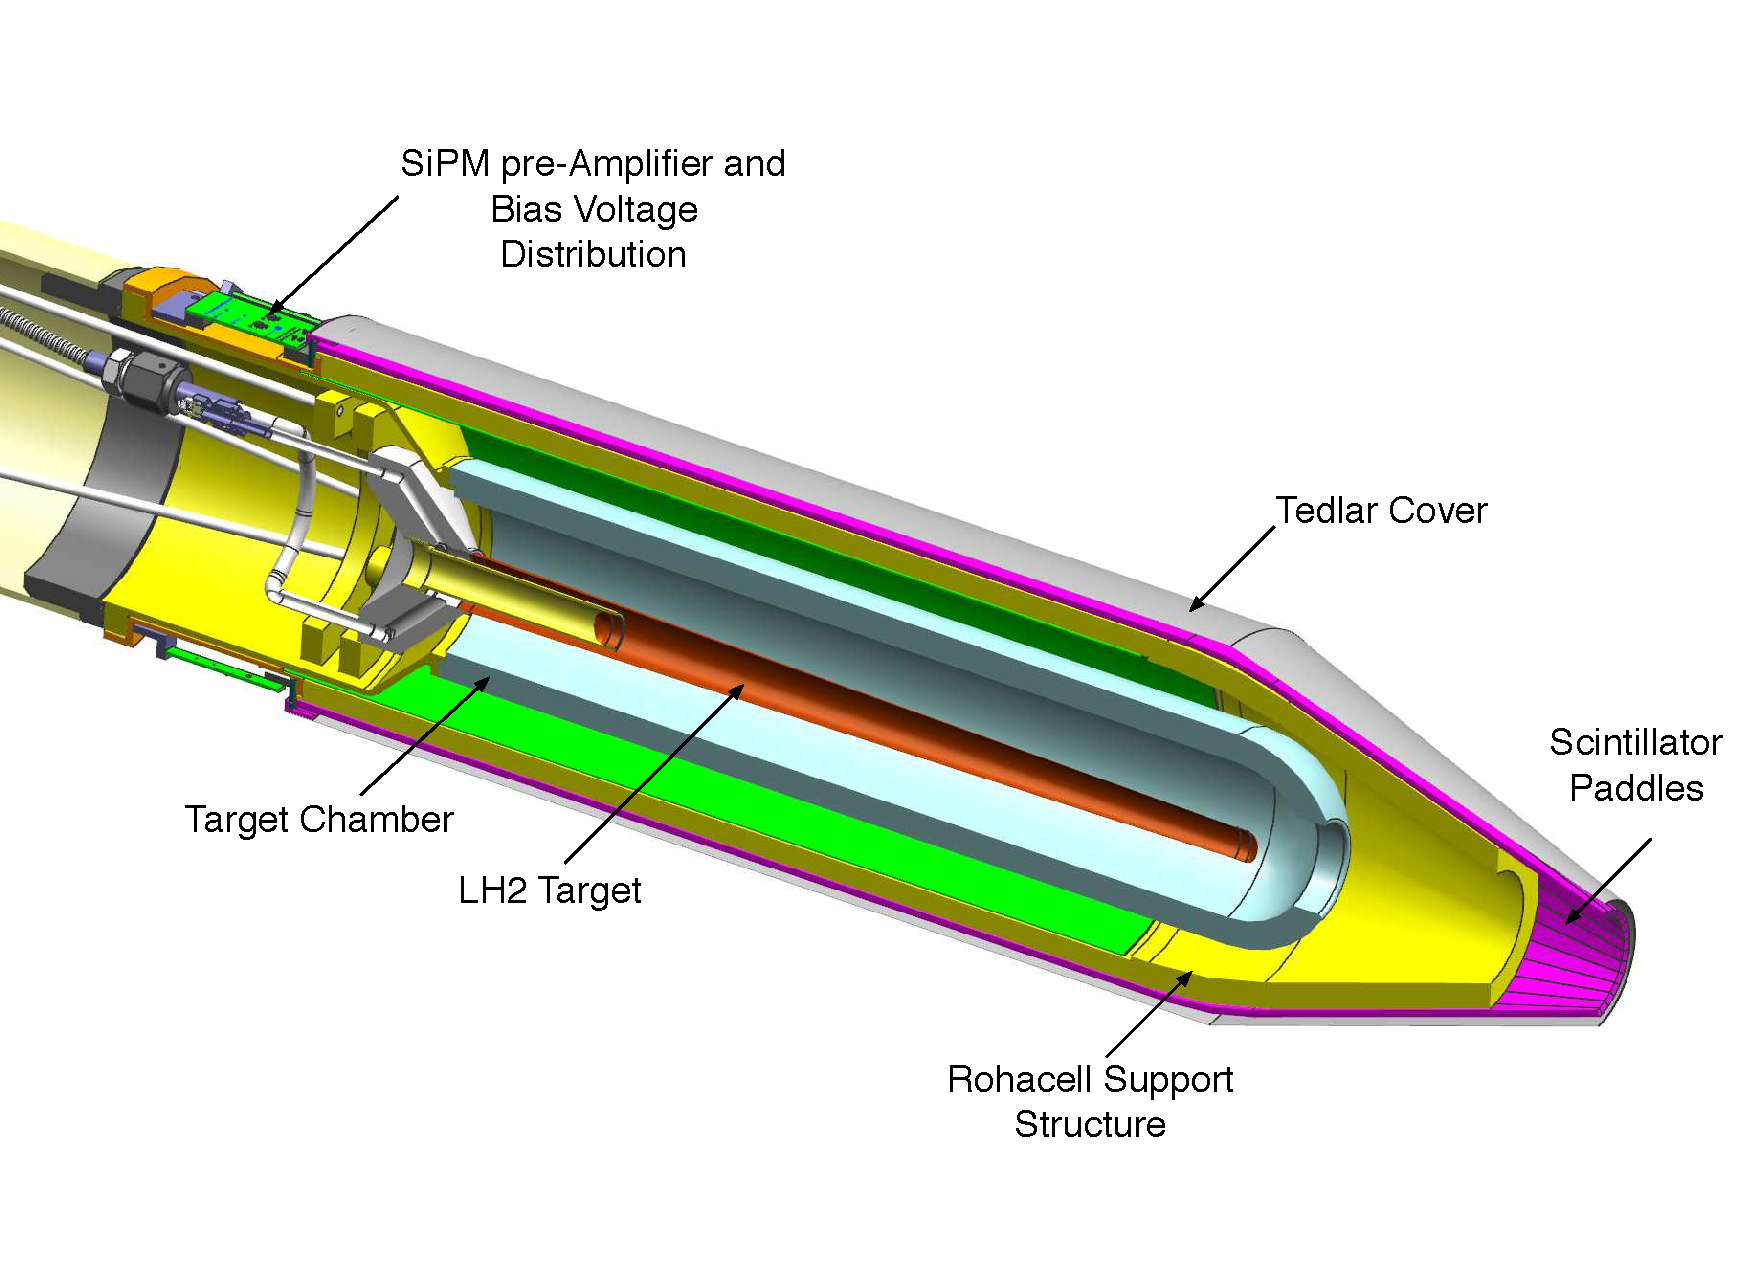
\includegraphics[width=1.0\columnwidth]{figures/start_counter_all.pdf}
\caption{The \gx{} Start Counter mounted to the liquid $\mathrm{H_2}$
  target assembly.  The beam goes from left to right down the central
  axis.\label{fig:st-overview-drawing}}
\end{figure}

\subsubsection{Detector Description}

The ST consist of 30 scintillator paddles arranged in a cylinder for most of
its length with a ``nose'' section that bends towards the beam line at
the downstream end. EJ-200 scintillator from Eljen
Technology\footnote{Eljen Technology, https://eljentechnology.com/products/plastic-scintillators.
	}
was selected. EJ-200 has a decay time
of 2.1~ns and an attenuation length of 380~cm. Silicon
photomultiplier (SiPM) detectors were use as light sensors [specs?]. These were
not affected by the 2 T[?] magnetic field produced by the GlueX
solenoid. The SiPMs were placed as close as possible to the upstream
end of each scintillator element to maximize light collection.

Each scintillator paddle started from stock 3~mm thick and 600 mm in
length. The paddles were bent at Eljen to create the nose section, and
then machined at McNeal Enterprises Inc.\cite{mcneal-reference} to
their final shape, including edges beveled at $6^\circ$ to minimize
loss of acceptance. The geometry for a single paddle is shown in
Fig.~\ref{figure:st-single-paddle-geometry}.

The scintillabor paddles are supported by a Rohacell closed-cell foam
structure. The Rohacell is 11 mm thick and is rigidly attached to an
aluminum support hub at its upstream end. The downstream support
extends partially into the nose section. The cylindrical length of the
Rohacell is further reinforced with three layers of carbon fiber, each
layer 650~$\mu$m thick. The assembly is made light-tigh with a Tedlar
wrapping. The Tedlar is attached to a plastic collar at the upstream
end. A summary of the materials used in the assembly are shown
schematically in Fig.~\ref{fig:st-materials}.

\begin{figure}[!htb]
  \centering
  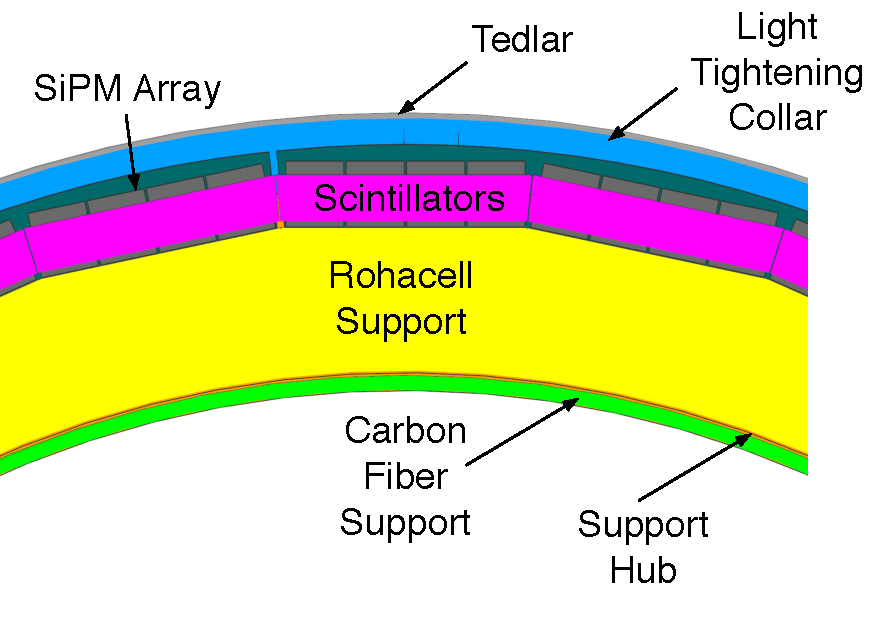
\includegraphics[width=1.0\columnwidth]{figures/st_materials.pdf}
  \caption{Start Counter materials.}
  \label{fig:st-materials}
\end{figure}

\subsubsection{Read-Out Electronics}

Each scintillator bar is read out with an array of four
magnetic-field-insensitive Hamamatsu S109031-050P multi-pixel photon
counters (MPPCs). Each MPPC consists of 3,600
$50 \times 50$ $\mu$m$^2$ avalanche photo-diode pixel counters
operating in Geiger mode. The signals from all pixels are summed. [no
  more mention of SiPM?] The scintillator is optically coupled to the
MPPCs through a 250 $\mu$m air gap. A schematic of the ST read-out electronics is shown in Fig.~\ref{fig:st-electronics}.

\begin{figure}[!htb]
  \centering
  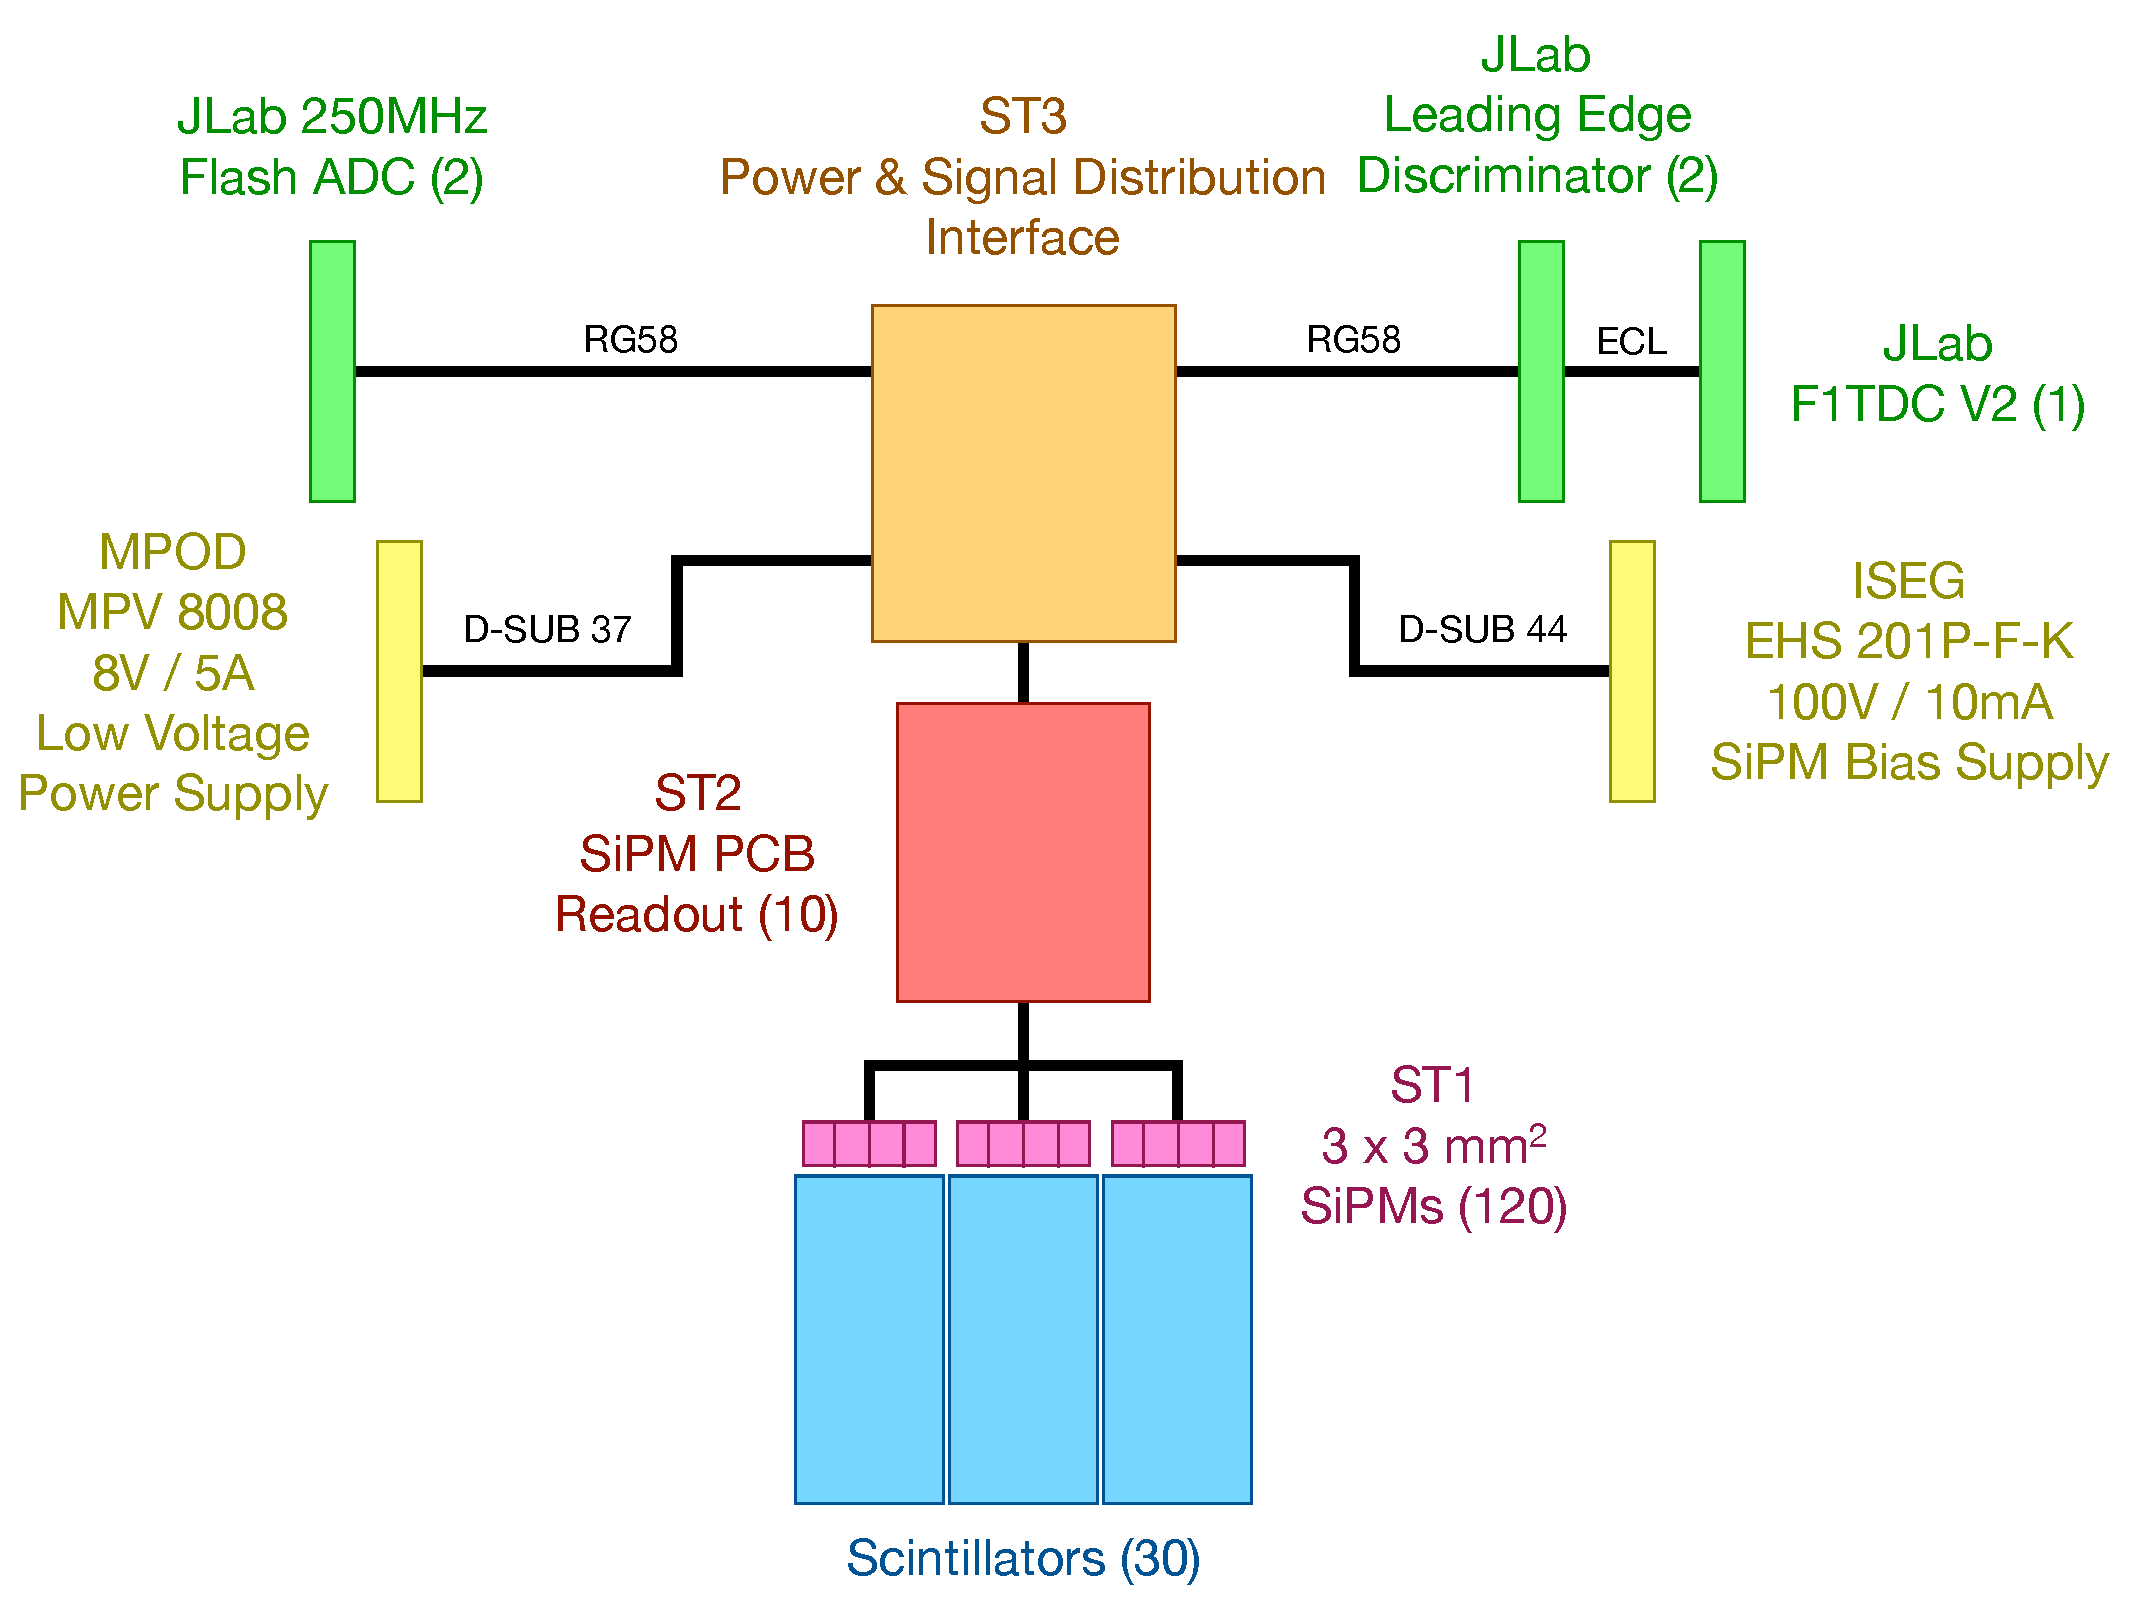
\includegraphics[width=1.0\columnwidth]{figures/st_electronics_diagram}
  \caption{Start Counter readout electronics diagram.  Numbers in 
    parenthesis indicate the total for the system.}
  \label{fig:st-electronics}
\end{figure}

The read-out electronics are deployed on three separate board designs,
``ST1,'' ``ST2,'' and ``ST3.'' The ST1 and ST2 boards are located
directly upstream of the end of the scintillator array, ST3 is located
further upstream, outside the bore of the solenoid magnet, adjacent to
the beam pipe.

The ST1 board houses the MPPCs themselves as well as a thermocouple for
temperature monitoring. Each ST1 board services three scintillator
paddles (twelve MPPCs per ST1 board). There are ten ST1 boards altogether. An ST1 board is shown in Fig.~\ref{fig:st-ST1}.

\begin{figure}[!htb]
  \centering
  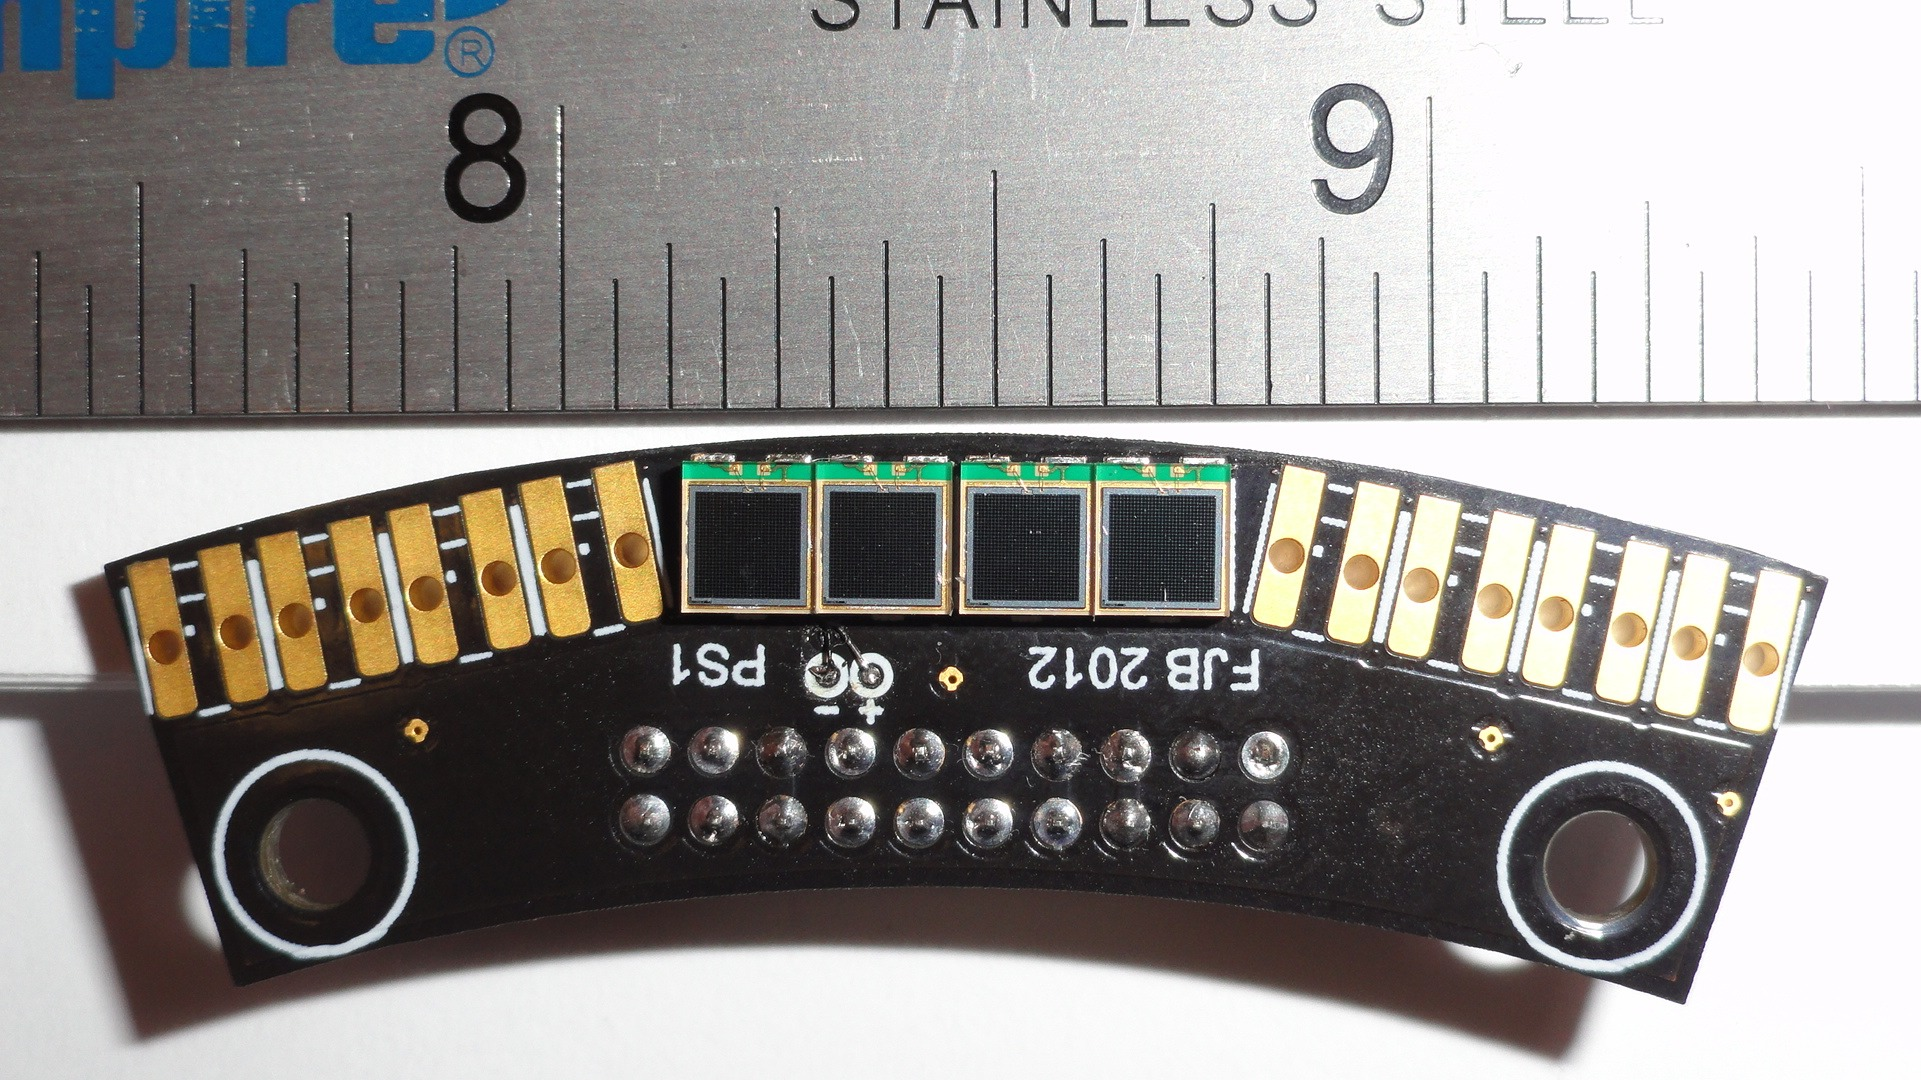
\includegraphics[width=1.0\columnwidth]{figures/st1_ruler}
  \caption{ST1 of Start Counter readout system.  Only the central array 
    is populated with SiPMs.  Approximately 72\% of the scintillator light 
    is collected at the upstream end.  The ST readout has 10 ST1 units in 
    total.  The ruler shown above is in inches.}
  \label{fig:st-ST1}
\end{figure}

For each ST1 board there is a corresponding ST2 board that services
all three electronic channels. For each channel there is a
pre-amplifier whose output is split. One side of the signal goes to a
buffer and then to a Flash ADC (FADC), the other goes to a
5$\times$~amplifier and is sent from there to a discriminator and TDC.

There is one ST3 provides an interface for distribution of low-voltage
power for the electronics and bias voltages for the MPPCs. It also
serves as a patch panel for the FADC, discriminator, and thermocouple
signal output cables.

\subsubsection{Calibration}

Calibrations are performed to correct measurements for the effects of
time-walk, light propagation time, and light attenuation

{\bf Time-Walk Correction}

Since the detector signal is sent to both a Flash ADC and a TDC, the time from the the FADC, which is largely independent of pulse amplitude, is used to measure the time walk seen by the TDC as a function of pulse amplitude as measured by the FADC. The resulting curve is fit to an empirical function to apply the correction and the procedure is done on a channel-by-channel basis.


\subsection[Time-of-flight counters (Beni)]{Time-of-flight counters \label{sec:tof}}
The Time-of-flight (TOF) detector is a wall of scintillators located about 5.5~m downstream from the target and covers 
an angular region from 0.6$^{\circ}$ to 13$^{\circ}$ in polar angle. The detector has two planes of
scintillator paddles stacked in the horizontal and vertical direction, respectively. Most paddles are 252~cm long and 2.54~cm
thick with a width of 6~cm. 
The scintillator material is EJ-200 from Eljen technology.
To accommodate the photon beam to pass through a central region of 12~cm by 12~cm is kept
free of any detector material giving rise to four short paddle detectors with a length of 120~cm around the beam hole
in each detector plane. These paddles also have a width of 6~cm with a thickness of 2.54~cm. In order to keep the
count rate of the paddles well below 2~MHz the two inner most full length paddles closest to the beam hole do have a reduced width of 3~cm.
Light guides from UV transmitting plastic provide the coupling space between the scintillator and the PMT and allow the 
magnetic shielding to protect the photo cathode by extending about 5~cm past the entrance window. All paddles are wrapped
with a layer of a highly reflective material DF2000MA from 3M followed by a layer of strong black Tedla film to
protect against external light sources. 
The main purpose of the detector is to provide fast timing for charged particles passing through the detector thereby providing information for particle identification and to the determine the event RF beam bunch of the photon that initiated the event.

\subsection{Electronics \label{sec:scelectronics}}
The full length scintillator paddles are read out on both ends using photo multiplier tubes (PMT) from Hamamatsu~\footnote{Hamamatsu Photonics "https://www.hamamatsu.com/us/en/index.html"}. These tubes of type H10534 have 10-stages and are complete assemblies with high voltage base, casing and $\mu$-metal shielding. Due to the significant stray field from the spectrometer solenoid magnet additional external
shielding based on soft iron is necessary to protect the PMTs from the magnetic field.
The high voltage (HV) to the PMTs is provided by CAEN HV modules of type A1535SN initially controlled by a CAEN SY1527 main frame
later upgraded to a SY4527.
The PMT output is connected to a splitter by a 50' long cables (WHAT TYPES?). The signal is split by
an passive splitter into two equal amplituded signals. One signals is directly connected to a flash ADC250~\cite{Dong:2007}
analog to digital converter (fADC) while the second signal passes first through a leading edge discriminator (LED) before connecting to 
a high resolution TDC VX1290A form CAEN~\footnote{CAEN "https://www.caen.it/"}. The digitizer electronics (fADC250 and TDC) are mounted
in VXS crates controlled by custom electronics as described in Section~\ref{sec:online}.
The threshold of the leading edge discriminator is controlled for each channel separately and has an intrinsic
dead time of about 25~ns.
The readout threshold for
the fADC250 is one single value for all channels on a single 16 channel board and is set to the same value for
all ADC modules in the TOF. The data from the fADC250 is provided by the FPGA algorithm and consists
of two words per channel with information about pedestal, signal amplitude, signal integral and timing.
The VX1290A TDC is a multi hit high resolution TDC with a buffer of 
up to 8 words per channel. The intrinsic dead time of a TDC channel is XX~ns. The timing resolution is about 25~ps per TDC count.
Since these TDCs provide the best time measurements in the GlueX detector the timing of the accelerator RF signal is also
digitized using this electronics.

\subsection{Calibration and monitoring \label{sec:sccalib}}
A detailed description of the TOF detector can be found in~\cite{GlueXTOFNIM}. Since the TOF detector consists of two
planes of narrow paddles oriented orthogonal to each other it is possible to calibrate the full detector independent
of any other external detector information. The overlap region of two full length paddles from the two planes define
a 6~cm by 6~cm area for most paddles with a few 3~cm by 3~cm areas close to the beam hole. The separation between
the two detector planes is minimal as they are mounted on top of each other and as such are only separated by their wrapping
material. While the time-difference TD between the two ends of a paddle is related to the hit position along the paddle
the mean-time MT is related to the flight time of a particle from the vertex to the paddle. Therefor the MT for two overlapping
paddles must be the same when they are hit by the same particle passing through both of them while the hit position in the horizontal (x) and vertical (y) dimensions are defined by TD of the two paddles. This relationship between paddles can be
explored to calibrate all paddles with respect to each other in a complete internally consistent way.

In a first step, however, all times have to be corrected for time-walk because of the use of LED discriminators which
introduces a time shift that depends on the signal amplitude. Because the signal amplitude together with its timing
in the fADC250 has been recorded as well this relation between time at threshold and signal amplitude can be parametrized and corrected for.

After all full length paddles with readout on both ends have been calibrated they can be used to as reference counters
the calibrate the remaining 8 paddles that do have only single-ended readout as they have to accommodate for the photon
beam to pass through the detector at zero degree. Again the fact that in any overlap region of two paddles from different
planes the flight time of the particle from the vertex to the detector is identical the MT of the full length paddle is used
as reference time for the time from the single ended paddle. This relation will result in a peaking distribution with the peak
location representing the timing offset of these single-ended readout paddles. Ensuring that the distribution of all offset
parameters together will have a distribution with a mean of zero will result in a timing calibration of TOF that is neutral
in time with respect to the time of any other detector in the GlueX spectrometer.

To test the calibration the time difference between the mean time of a reference paddle of choice with respect to 
all other long paddles from the other plane is calculated for hits associated with reconstructed charged tracks that hit
the reference paddle. The resulting distribution of these differences is shown in Fig.~\ref{fig:mt_diff}. Assuming that
all paddles have the same timing resolution an average time resolution for the reference counter can be determined 
and is found to be  96~ps$=\frac{136}{\sqrt{2}}$~ps, assuming a Gaussian distribution.
\begin{figure}[tbp]
\begin{center}
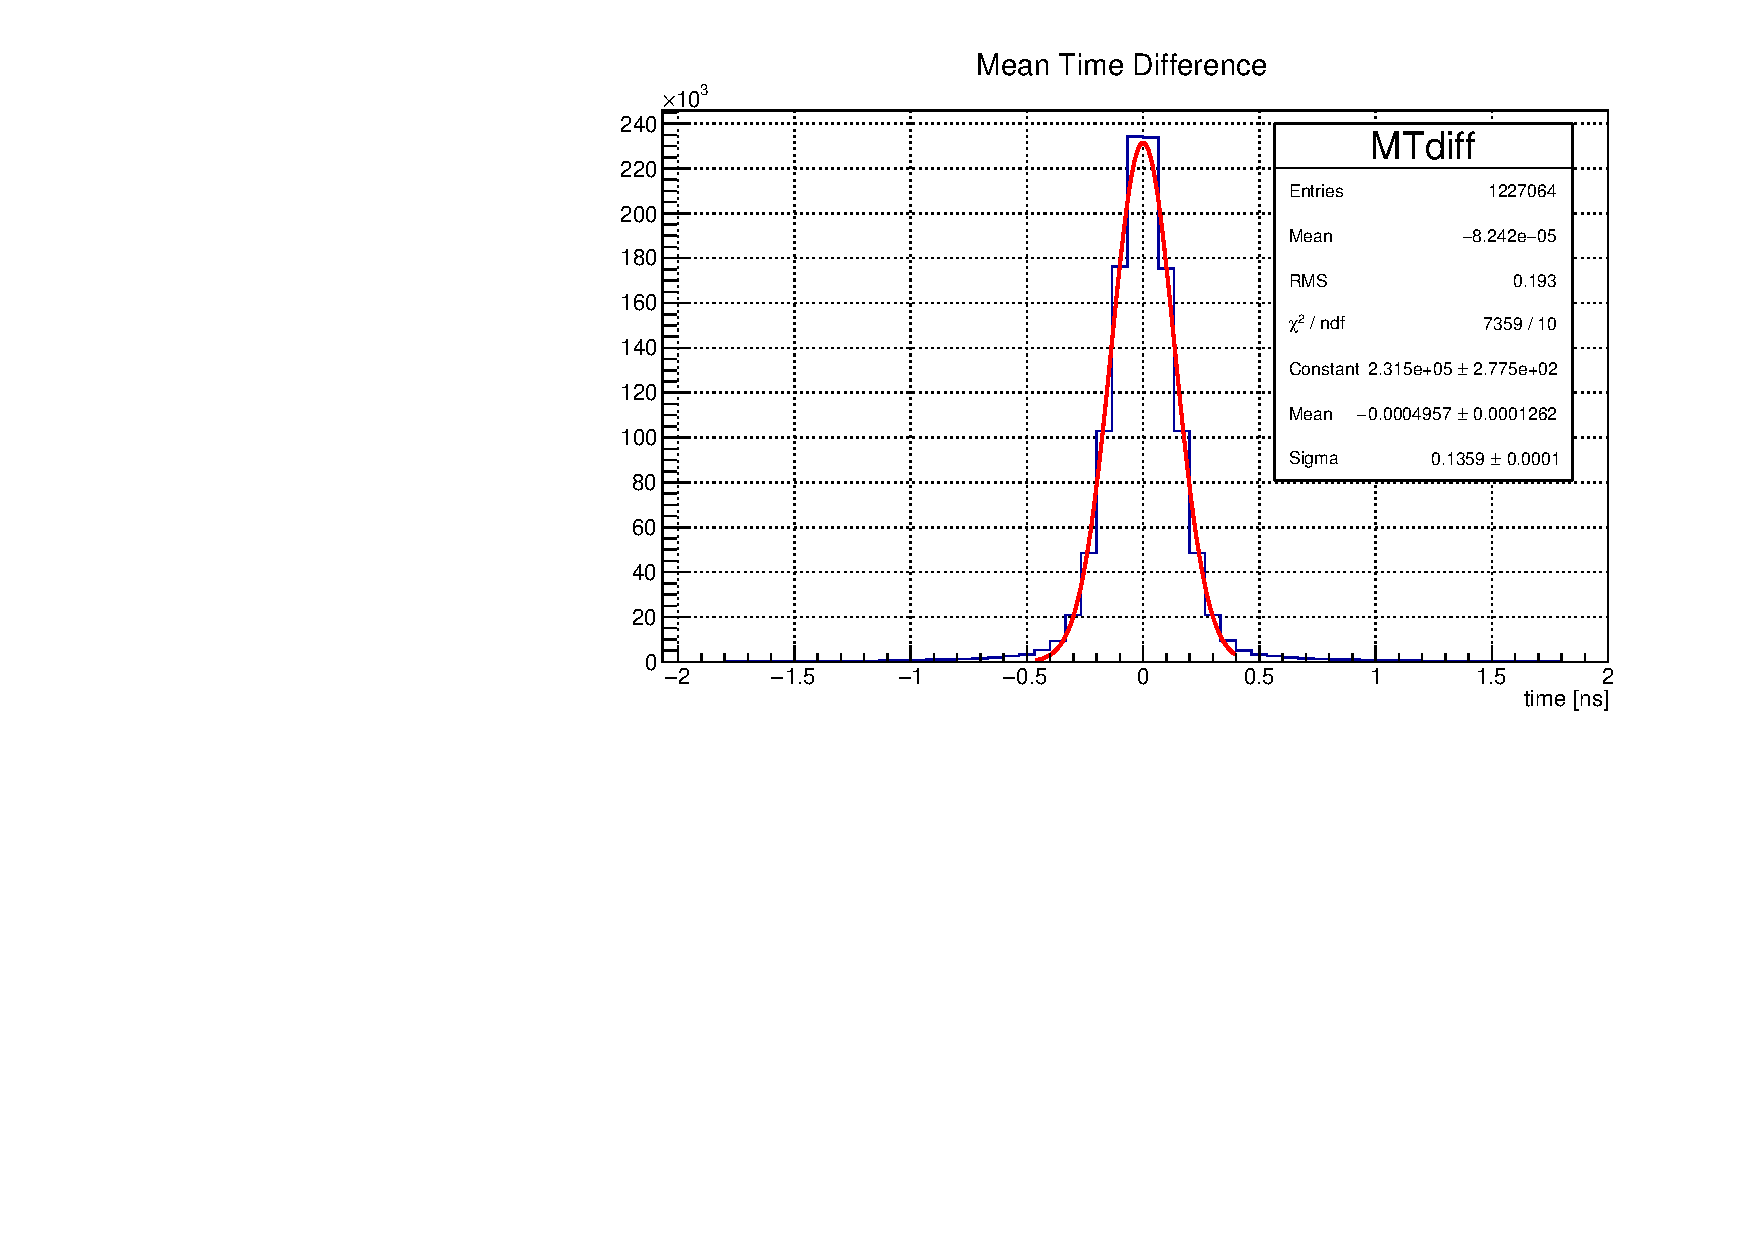
\includegraphics[width=0.8\textwidth]{figures/mt_diff_fullTOF.pdf}
\caption{\label{fig:mt_diff} Mean time difference between one long paddle of one plane with all other long paddles
of the other plane. (Color online)}
\end{center}
\end{figure}
\subsection{Performance \label{sec:scperformance}}
To investigate the performance of the TOF detector for its PID capability it is important to include the relative number of
particle types within the event sample. Here events are selected that do have at least three fully reconstructed charged tracks in the final state with at least one of these tracks intersecting with the TOF detector. The number of pions in such samples will
be much larger than for kaons. The number of protons will be certainly larger than kaons since the data is taken with a hydrogen 
target. Looking at the distribution of $beta$ of these tracks as a function of momentum it is easy to identify the bands
from protons, kaons and pions (see Fig.~\ref{fig:betavsp}). 

Looking at $\beta$ at two specific track momenta of 2~GeV/c and 4~GeV/c, respectively (see Fig.~\ref{fig:betaproj}) is very illustrative to see the limitations
of the TOF detector in terms of PID. At 2~GeV/c particle momentum the TOF detector provides about a 4$\sigma$ separation between
the pion,lepton peak and the kaon peak. This is sufficient to identify tracks with a $\beta$ of 0.97 or lower as kaons with a very
high certainty. However, at a $\beta$ of 0.98 the probability of the track begin a kaon is less than 50\% mainly due to the fact
that the abundance of pions is close to an order of magnitude larger than kaons. The protons on the other hand are very well
separated from the other particle types and can be identified as such with high confidence over the full range in $\beta$.
At a track momentum of 4~GeV/c this has changed and represents the limit at which the TOF can identify protons with high confidence. Again the separation between the large peak containing now pions, kaons and leptons is separated from the proton
peak by about 4$\sigma$, while the relative abundance in this case is about a factor of 4. As a consequence a 4~GeV/c momentum
track with a $\beta$ of 0.975 is most likely a proton with a small probability of being a pion. At a $\beta$ of 0.98 such
a track has a similar probability for being a proton or a pion.
\begin{figure}[tbp]
\begin{center}
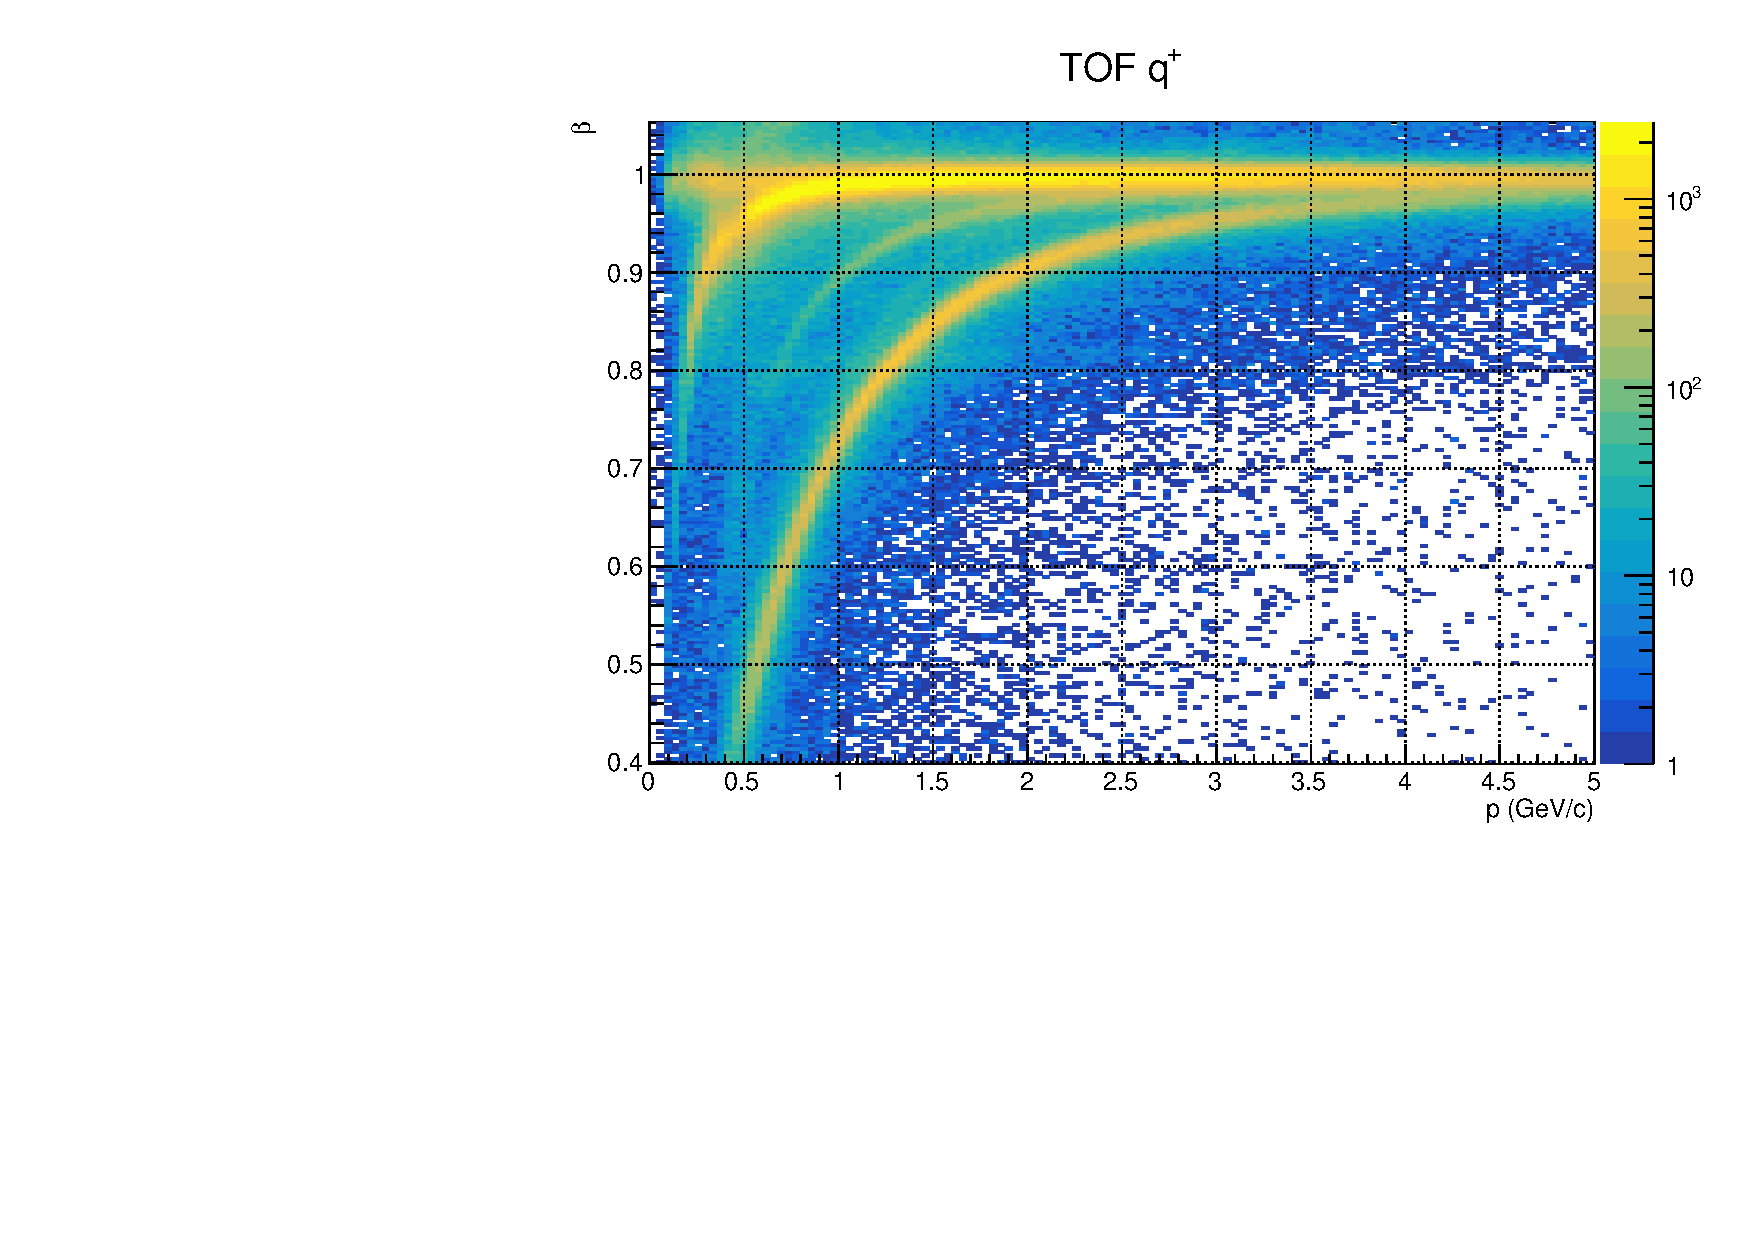
\includegraphics[width=0.8\textwidth]{figures/beta_vs_p_positivetracks.pdf}
\caption{\label{fig:betavsp}$\beta$ of positive charged track vs track momentum. The color coding of the third dimension
is in logarithmic scale.(Color online)}
\end{center}
\end{figure}

\begin{figure}[tbp]
\begin{center}
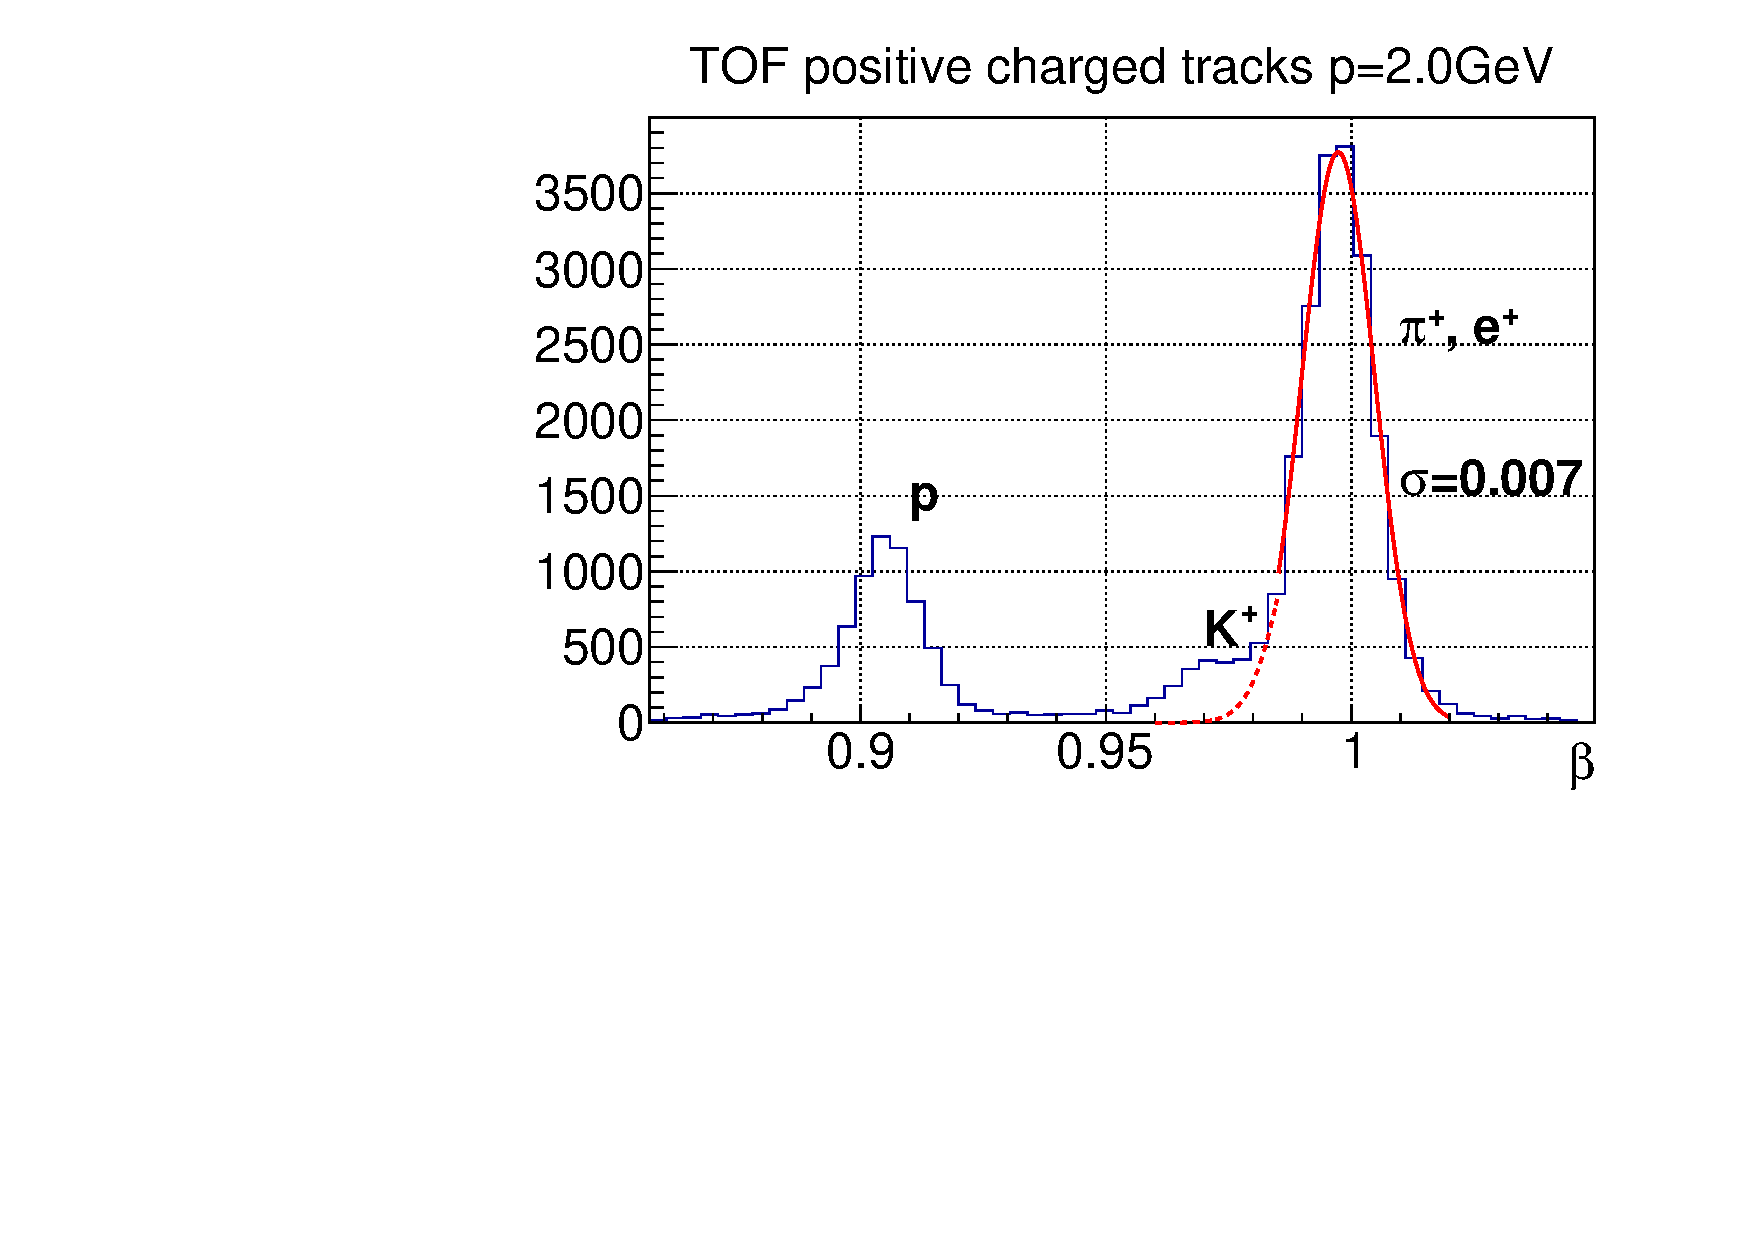
\includegraphics[width=0.45\textwidth]{figures/TOF_postracks_2000mev.pdf}
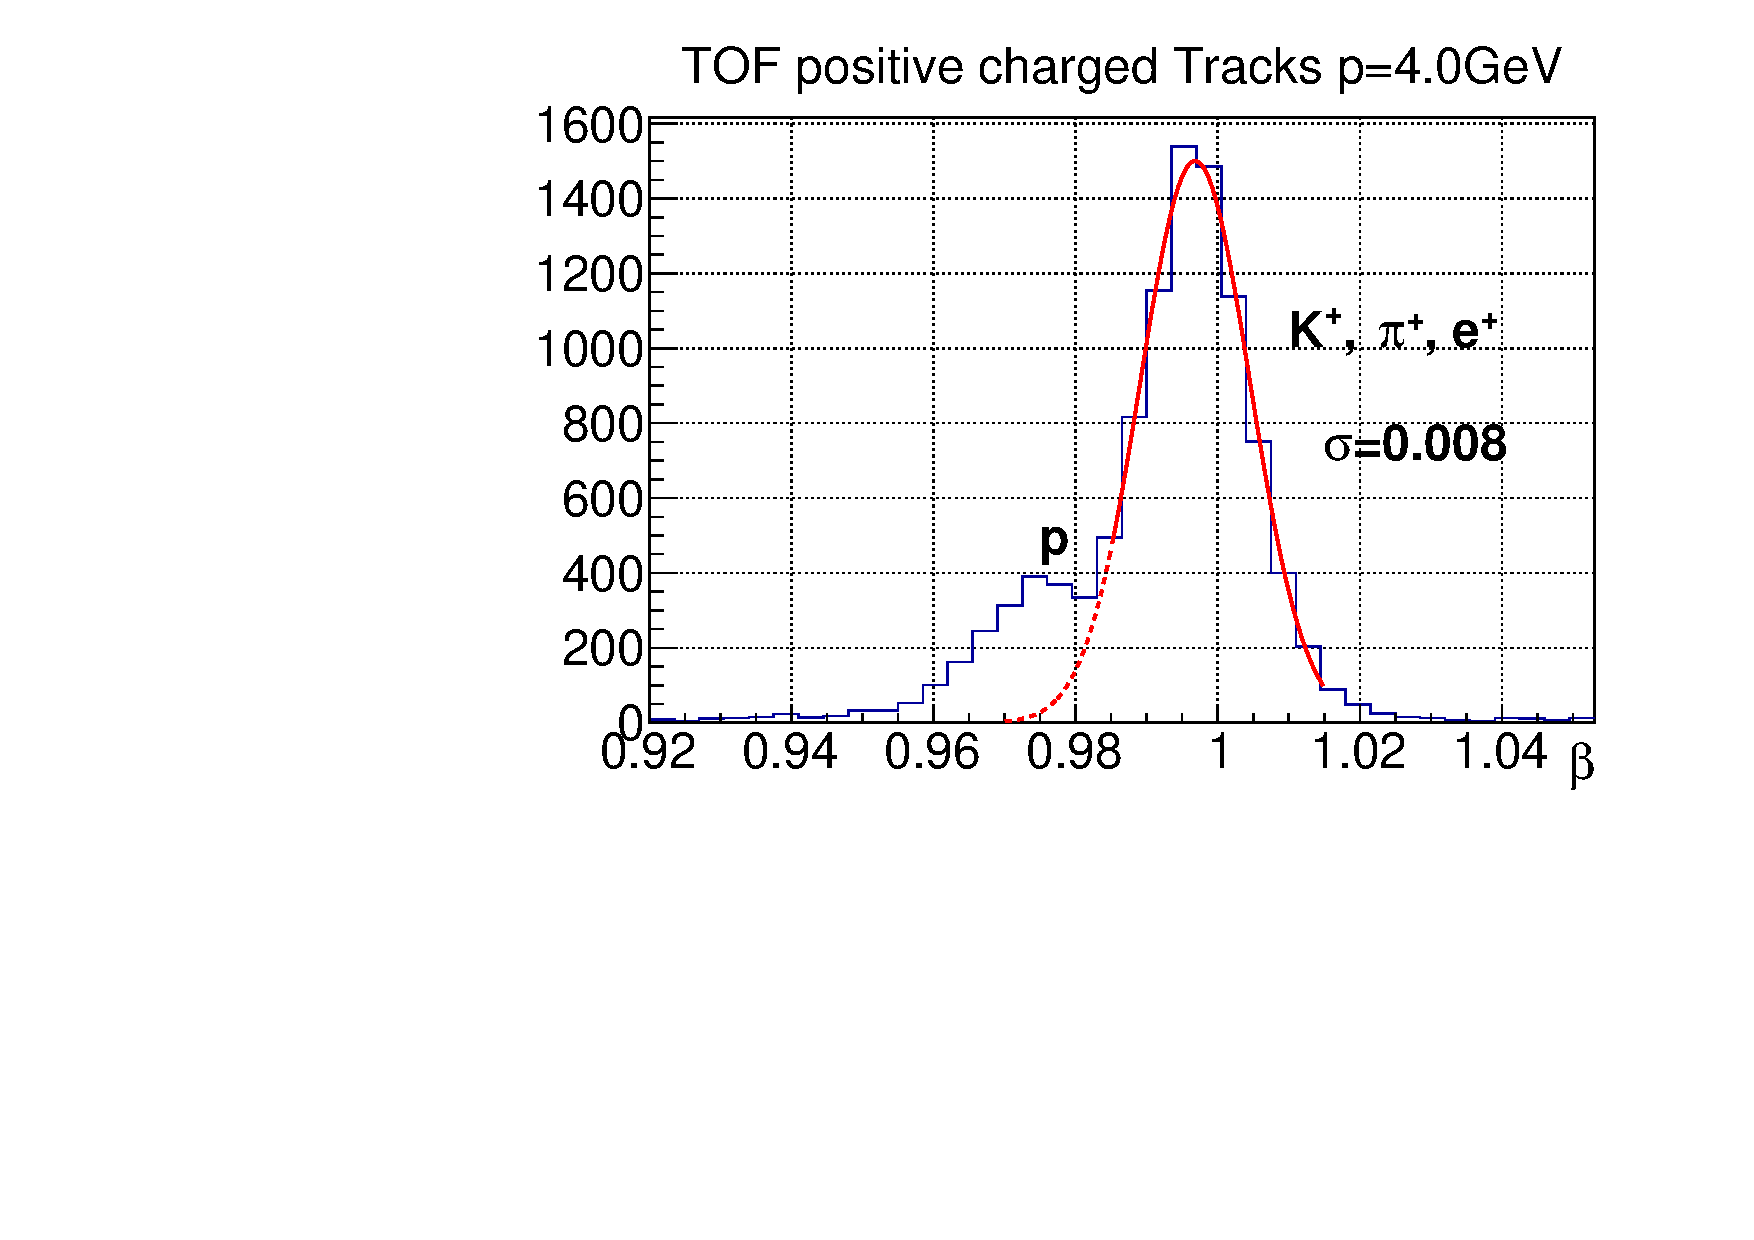
\includegraphics[width=0.45\textwidth]{figures/TOF_postracks_4000mev.pdf}
\caption{\label{fig:betaproj}$\beta$ of positive charged track with 2~GeV/c momentum (left) and with 4~GeV/c (right).}
\end{center}
\end{figure}

\subsection{Summary \label{sec:scsummary}}
The TOF detector in the forward region of the GlueX spectrometer provides high resolution timing information that contributes
to the identification of the RF beam bucket of the beam photon that initiated the event. In combination with the charged
track reconstruction TOF hits can be matched to such tracks to determine $\beta$ and as such give access to the particle
mass of the track. Protons can be identified with reasonable confidence up to momenta of 4~GeV/c while kaons can be
identified up to momenta of 2~GeV/c.

%=======================+=========================
%==============  Trigger and DAQ   ================
%=================================================\

\section{Trigger and data acquisition  \label{sec:trigdaq}}
\subsection{Architechture \label{sec:trigdaqarchichecture}}
\subsection{Triggers \label{sec:trigdaqtriggers}}
\subsection{Data logging \label{sec:trigdaqdata}}
\subsection{Rate capability \label{sec:trigdaqrate}}
\subsection{Performance \label{sec:trigdaqperformance}}

%=======================+=========================
%================  Controls  ================
%=================================================

\section[Slow controls]{Slow controls \label{sec:controls}}
\GX{} requires the ability to monitor 
and control tens of thousands of different variables that define the state of the experimental hardware. Different variable values need to be acquired, displayed, archived, and used as inputs to control loops continually with a high degree of reliability. For \gx~ we archive approximately 90,000 variables, and monitor many more.

\subsection{Architecture \label{sec:controlsarchitechture}}
The \gx{} slow control system consists of three layers. The first layer consists of the remote units such as high voltage or low voltage power chassis, magnet power supplies, temperature controller, LabView applications, and PLC-based applications, which directly interact with the hardware and contain almost all of the control loops. The second layer is the Supervisory Control and Data Acquisition (SCADA) layer which is implemented via approximately 140 EPICS Input/Output Controllers (IOC's). This layer provides the interface between low level applications and higher level applications via the EPICS ChannelAccess protocol. The highest level, referred as Experiment Control System (ECS), contains applications such as Human-Machine Interfaces (HMIs), the alarm system and data archiving system. This structure allows for relatively simple and seamless addition and integration of new components into the overall controls system.    

\subsection{Remote Units \label{sec:controlsinterface}}
\gx{} uses a variety of commercial units to provide control over the hardware used in the experiment. For instance, most of the detector high voltages are provided by the CAEN SYx527 voltage mainframe\footnote{https://www.caen.it/subfamilies/mainframes/} while the low and bias voltages are provided by boards residing in Wiener MPOD chassis\footnote{http://www.wiener-d.com/sc/power-supplies/mpod--lvhv/mpod-crate.html}. These two power supply types provide most of the voltage with the exception of Tagger Microscope and Forward Calorimeter where custom systems were developed which provide voltage regulation and interact with the EPICS-based layer through higher level interfaces using custom protocols, see Sections.~\ref{sec:TAGM} and \ref{sec:fcal} for more details.  

Various beam line devices need to be moved during beam operations. We use stepper motors to move motorized stages via Newport XPS universal multi-axis motion controllers\footnote{https://www.newport.com/c/xps-universal-multi-axis-motion-controller.} that allow for execution of complex trajectories involving multiple axes. All of the stage referencing, motion profile computations and encoder-based closed-loop control occur within the controller chassis after the basic parameters such as positions and velocities are provided by the user via TCP/IP based interface to EPICS.   

While installing complex systems, such as a superconducting magnet, we have developed a custom controls system with a large number of input and output channels, and sophisticated logic suited for the particular system. For those cases we mostly  used Allen-Bradley CompactLogix and ControlLogix PLC systems\footnote{https://ab.rockwellautomation.com.}. These systems are designed for industrial systems, allow for a modular design, and provide high reliability and require minimal maintenance. All of the controls loops are programmed within the PLC application. These PLC's are interfaced with EPICS through the TCP/IP EtherNet/IP proprietary protocol to allow the higher level applications access to process variables served by the PLC's.  

The cryogenic target and the superconducting solenoid employ National Instruments LabView applications. The controls of the target are implemented using custom-made and vendor-supplied hardware that include built-in remotely-accessible control systems and a NI CompactRIO\footnote{https://www.ni.com/en-us/shop/compactrio.html} chassis. This chassis communicates with the hardware and serves variables using an internal ChannelAccess server and an EPICS IOC running on the CompactRIO controller, as described in detail in Sec~\ref{sec:target}. We also use a National Instruments PXI high performance system\footnote{https://www.ni.com/en-us/shop/pxi.html} to collect data from different sensors as described in Sec.~\ref{sec:solenoid}. 

\begin{landscape}
 \begin{figure}[tbp]
\begin{center}
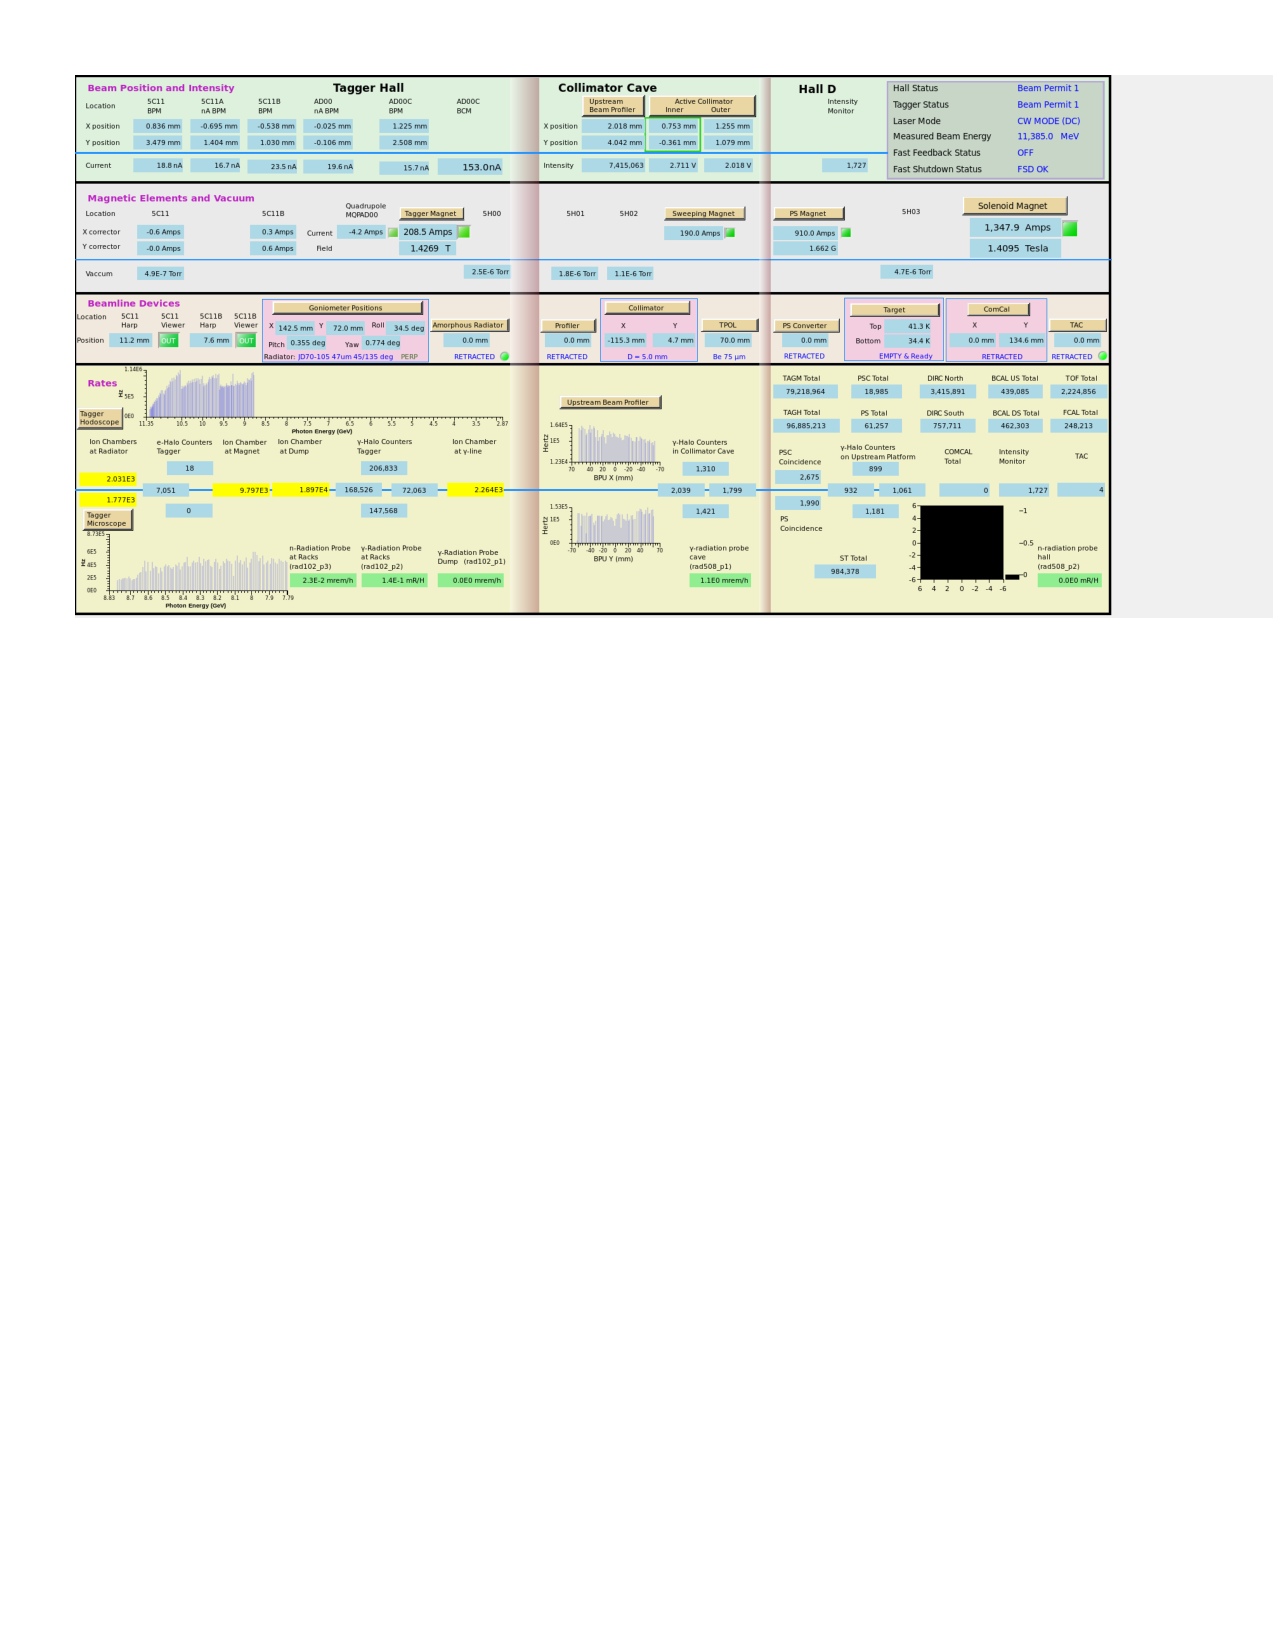
\includegraphics[height=10cm,bb=35 480 535 760,clip=true]{figures/GlueX_CSS_overview.pdf}
%\includegraphics[height=8cm,clip=true]{figures/GlueX_CSS_overview.pdf}
\caption{Top-level graphical interface for the beamline. This screen provides information on beam currents and rates, radiators, magnet status, target condition, background levels, etc.
\label{fig:GlueX_CSS_overview}
}
\end{center}
\end{figure}
\end{landscape}

\subsection{Supervisory Control and Data Acquisition layer \label{sec:archiver}}
The Supervisory Control and Data Acquisition (SCADA) layer is the middle layer that distributes the process variables allowing the higher level, and sometimes lower level, applications to use various process variables of the Hall-D control system. This layer is based on EPICS and uses the ChannelAccess protocol to publish the values of the variables over Ethernet. And because the accelerator controls also uses EPICS, this allows us to efficiently exchange the information between the experiment and accelerator operations. There are several dozen of software IOC processes running on hosts in the experiment control room that collect data from different components of the lowest layer. Each of these IOCs is configured to communicate using the protocol appropriate for the remote units from which it needs to exchange data. For instance the IOC controlling the voltage for the FDC detector needs to be able to communicate with Wiener MPOD and CAEN SYx527 voltage chassis. Although the middle layer is there mostly to distribute the data between different applications it also contains some EPICS-based applications running on IOC's that provide different control loops and software interlocks.  For instance, the low voltage power supplies for the FDC detector (see Sec. \ref{sec:fdc}) are shut off if the temperature or the flow of the coolant in the chiller falls outside of required limits. 
\subsection{Experiment Control System \label{sec:alarms}}
The highest level of controls contains the applications that archive data, display data in interactive GUIs and as stripcharts, alarm and notify shift personnel and experts in case problems occur, and interface with the CODA-based data acquisition system described is Sec.~\ref{sec:daq}.
An example of a GUI is provided by the beamline overview screen, shown in Fig.\,\ref{fig:GlueX_CSS_overview}. Many of the buttons are active and allow access to other GUIs.
The display management and the alarm system for \gx{} controls is based on Controls System Studio (CSS),\footnote{http://controlsystemstudio.org/}  which is an Eclipse-based toolkit for operating large systems and it is well suited for systems built on EPICS. Although CSS provides its own archiving engine and stripcharting tools we used the MYA archiver~\cite{Slominski:2009icaleps} provided by the JLAB accelerator software group with its tools for displaying the archived data as a time-series. The display management for \gx{} controls is done within the CSS BOY~\cite{Chen:2011icaleps} environment and allows system experts to build sophisticated control screens using standard widgets. The alarm system is based on the CSS BEAST\cite{Kasemir:2009icaleps} alarm handler software, which alerts the shift personnel about the problems with the detector. It also notifies system experts if the problems are not resolved by shift personnel.   
%=======================+=========================
%================  Online  ================
%=================================================

%------------------------------------------------------------------
\section[Online computing system]{Online computing system \label{sec:online}}

This section describes the \GX ~software and computing systems that are used for both data monitoring and transport to the tape system for permanent storage.

%------------------------------------------------------------------
\subsection{Monitoring \label{sec:onlinemonitoring}}

The Online Monitoring system consists of multiple stages that provide for immediate monitoring of the data, as well as near-term monitoring ($\sim$hours after acquisition). The immediate monitoring is based on the \textit{RootSpy} system\cite{rootspy} written for use in \GX, though its design is not \GX ~specific. Figure \ref{fig:online_monitoring_processes} shows a diagram of the processes involved in the RootSpy system and how they are coupled to the DAQ system. The Event Transfer System (ET) is part of the CODA DAQ system\cite{coda} and is used to extract a copy of a portion of the data stream without interfering with the DAQ itself. The monitoring system itself uses a secondary ET in order to minimize connections to the RAID server that is running the Event Recorder process.

\begin{figure}[tbp]
\begin{center}
\includegraphics[width=0.99\textwidth, clip,trim=1.5cm 0.9cm 1.7cm 0.8cm]{figures/online_monitoring_processes.pdf}
\caption{\label{fig:online_monitoring_processes}Diagram of the various processes distributed across several computers in the counting house that make up the online monitoring system. DC, EB, and ER represent the Data Concentrator, Event Builder, and Event Recorder processes respectively in the CODA DAQ system.}   
\end{center}  
\end{figure}

The monitoring system is run on a small farm of computers\footnote{The online monitoring farm consists of eight 2012 era Intel x86\_64 computers with 16 cores+16ht plus six 2016 era Intel x86\_64 computers with 36 cores + 36ht. The monitoring farm uses 40 Gbps (QDR) and 56 Gbps(FDR) IB for the primary interconnect. Note that the DAQ system uses a separate 40 Gbps ethernet network that is independent of the farm.} in the counting house, each processing a small part of the data stream. In total, about 10\% of the data is processed for the low level occupancy plots while roughly 2\% is fully reconstructed for higher level analysis. The CODA ET software system is used to distribute the data among the farm computers. Each farm node generates histograms which RootSpy gathers and combines before displaying them to shift workers in a GUI.
%Figure \ref{fig:online_monitoring_rootspy} shows a screen capture of the main RootSpy GUI window along with a window displaying the reference plot for the currently displayed image.
Plots are displayed via a set of ROOT macros, each responsible for drawing a single page. Most macros divide the page into multiple sections so that multiple plots can be displayed on a single page. Figure \ref{fig:online_monitoring_PID} shows an example of a high level monitoring plot where four invariant mass distributions are shown with fits. Values extracted from the fits are printed on the plots for easy quantitative comparison to the reference plot. 

Shift workers are presented with live plots alongside reference plots for comparison. Shift workers may assign a live plot as the new reference using a button on the RootSpy GUI. Relevant experts for the given plot are notified via e-mail when a new reference is made, thus providing for expert oversight of the reference plots.

ROOT macros are passed into the RootSpy GUI using the same xMsg\cite{xmsg} publish subscribe messaging system used to transport histogram objects. The macros are compiled into plugins as C++ strings by the build system. The build system recognizes ROOT macro files in the plugin source directory (via the .C suffix) and automatically generates C++ code that contains the macro and code to register it with the RootSpy system. This is done to ensure that a macro is always in sync with the histograms it displays since the former is linked in the same binary as the routines that produce the latter.

\begin{figure}[tbp]
\begin{center}
\includegraphics[width=0.99\textwidth]{figures/online_monitoring_PID.pdf}
%\includegraphics[width=0.99\textwidth, clip,trim=0.6cm 0.0cm 1.1cm 0.0cm]{figures/online_monitoring_PID.pdf}
\caption{\label{fig:online_monitoring_PID}Invariant mass distributions showing $\pi^\circ$, $\omega$, $\rho$, and $\phi$ particles. These plots were generated online in about 1hr 40min by looking at roughly 2\% of the data stream.}   
\end{center}  
\end{figure}

In addition to the RootSpy GUI, several other client programs exist that consume the histograms being produced by the RootSpy system. One of these is the RSTimeSeries program. This program periodically runs a set of macros that contain special calls to insert data into an InfluxDB time series database. This provides a web-accessible strip chart of detector hit rates and reconstructed quantities (e.g. number of $\rho$'s per 1k triggers). The RSArchiver program gathers summed histograms and periodically writes them to a ROOT file for permanent storage. The archive file is later used to generate a set of image files that are displayed in the Plot Browser\footnote{https://halldweb.jlab.org/data\_monitoring/Plot\_Browser.html.} website. Plot Browser allows for easy comparison of plots for different runs as well as with similar plots produced during offline analysis. The first five files (100GB) of each run are automatically pinned to disk in the JLab Computing Center after being transported there for permanent tape storage. Jobs are automatically submitted for these files to the JLab SciComp farm to perform full reconstruction. The results are displayed in Plot Browser under the title ``Incoming Data.''


%------------------------------------------------------------------
\subsection{Data Transport and Storage \label{sec:onlineprocessing}}

\GX ~Phase I generated production data at rates up to 650MB/s. The data were temporarily stored on large RAID-6 disk arrays and then copied to an LT0 tape system for long term storage. Two RAID servers, each with four partitions were used in the Hall-D counting house. The partition being written to was rotated between runs through the use of symlinks. This helped to minimize head thrashing on disks by only reading from partitions not currently being written to. Partitions were kept approximately 80\% full and older files deleted only as needed to maintain this. This was to allow the monitoring farm easy access to the files for times when the beam was down. An additional copy of the first 3 files ($\sim1.5\%$) of each run was made to a smaller RAID disk so that an easily accessible sample of each run could be maintained in the counting house.

The data volumes stored to tape are shown in table \ref{tab:online_data_volumes} in units of petabytes(PB). Lines marked ``actual'' are values taken from the tape storage system. The line marked ``model'' comes from the \GX ~computing model\cite{gx3821}.

\begin{table}[]
    \centering
    \begin{tabular}{|l|c|c|c|c|c|}
    \hline
                           & \textbf{2016}  & \textbf{2017}  & \textbf{2018} \\
    \hline
    actual (raw data only) & 0.624 & 0.914 & 3.107 \\
    \hline
     model (raw data only) &       & 0.863 & 3.172 \\
    \hline
    \hline
    actual (production)    & 0.55  & 1.256 & 1.206 \\
 %   \hline
 %    model (production)    &       & 0.607 & 3.084 \\
    \hline
    \end{tabular}
    \caption{\GX ~Data volumes by year. All values are in petabytes(PB). Most years include two run periods. The line marked \textit{model} is calculated from the \GX ~Computing Model\cite{gx3821}. ``Raw data only'' represents data generated by the DAQ system (not including the backup copy). ``Production'' represents all derived data including reconstructed values and ROOT trees. }
    \label{tab:online_data_volumes}
\end{table}


\clearpage   % avoid formatting problems with empty sections
%=======================+=========================
%================  Reconstruction  ================
%=================================================


\section[Event reconstruction]{Event reconstruction \label{sec:reconstruction}}

% Copy from GlueX-doc-3108
% "Production and Analysis of GlueX Data"
% TODO: UPDATE for 2017

During and after experimental running, GlueX used the computer center batch farm at Jefferson Lab to perform data monitoring, event reconstruction, and physics analyses.  For data monitoring, we studied the detector hit occupancies, calibration and reconstruction quality, and experimental yields and resolutions for several physics channels.  We monitored a subset of the data as soon as it was saved to tape, submitting batch farm jobs via cron jobs.  Every few weeks, we performed monitoring launches on a subset of the data to study improvements from ongoing calibrations and reconstruction software improvements.  The histograms produced by these monitoring jobs were displayed on a web site and ROOT files were available for download, so that collaborators could easily study the quality of the data. 

Every few months we performed a major reconstruction launch over all of the data, linking the hits in the various detector systems to reconstruct particles in the physics events.  Monitoring plots from these launches were also published to the web. Finally, we regularly performed analysis launches over the reconstructed data, where one JANA plugin was used to filter out reactions that were previously specified by users on a web form. The results of these launches were saved in reaction-specific ROOT TTrees for further analysis. For all launches, JANA was run multithreaded to make efficient use of the available computing resources.  %Figure~\ref{fig:offline_monitorA} shows the multithreaded scaling from our monitoring launches is near the theoretical limit.  SWIF is used to manage the batch farm jobs, and is queried to study the performance of the launches.  Figure~\ref{fig:farm-time} shows how many batch farm jobs were in each processing state as function of time our latest reconstruction launch.
All file outputs were written to a write-through cache system, which is ultimately backed up to tape.  

The series of steps in the production of GlueX data will be describe in the following. In its initial phase, GlueX recorded more than XXX separate runs with a unique run number, which have a total data footprint of about 5 petabytes. The data acquisition system saved the data in $19$ gigabyte files, with all physics quality runs consisting of multiple files (typically $100$ or more). Figure~\ref{fig:production_overview} shows an overview of the different production steps for GlueX data. 

\begin{figure}[h!]\centering
\includegraphics[width=0.8\textwidth]{figures/Production_generic.pdf}
\caption[]{\label{fig:production_overview}Production flow chart for GlueX data.} 
\end{figure}

\subsection{Calibration pass \label{sec:reccalibration}}

Two types of calibration jobs are running, depending on the complexity of the calibration procedures.  Simple, well-understood calibrations such as timing alignment between individual channels and subdetectors or drift chamber gain and time-to-distance calibrations, can be performed with one file of data per run.  These procedures are run either in the online environment or on the batch farm, and can be run several times as needed due to improvements in reconstruction algorithms or other calibrations.

More complicated calibration procedures, such as calorimeter gain calibration, require more data and are often iterative procedures, requiring several passes through the available data.  The raw data is processed on the batch farm as it comes into the computer center to produce the outputs needed for these procedures, either in the form of histograms or reduced skims in EVIO or ROOT tree format.  Many of these output require that charged particle tracks be reconstructed, but because of the computationally intensive nature of track reconstruction at GlueX, the available computing resources at JLab are insufficient for fully reconstructing all of the raw data as it comes in.  Therefore, only about $10-20$\% of the data has the full suite of calibration procedures applied.  The rest has a limited set of procedures, mostly focused on separating out events collected by specialized triggers. 
The individuals responsible for specific detector calibrations are then responsible for analyzing the skimmed data.

\subsection{Monitoring pass \label{sec:recmonitoring}}

The red-colored box at the top represents the experimental data that has been copied to the computer center. The small part of the box represents the first five files of each run, which are run through the offline monitoring processes. These monitoring jobs are first run during the run to check the quality of the data, but are also run after major changes to calibrations or software to validate those changes. These jobs produce both Reconstructed Events Storage (REST) files and root histogram files for checking the detector and reconstruction performance.

\subsection{Reconstruction pass \label{sec:recreconstruction}}

When the data is sufficently well calibrated, we carry out a full production of the physics quality data. In the total GlueX data set, about 1400 of the
runs were deemed physics quality. The remaining were short runs which were related to engineering and commissioning tests of the experiment. We note that while this number is small compared to the total number of runs, it is the vast majority of all data recorded during the running period, representing about 3 petabytes. All of these files are reconstructed and produce more than $500$ terabytes of REST data files. The large reduction is size from collected event data to physics data files allows us to  more quickly and efficiently carry out physics analyses on the data.
%, and is also small enough to be fully exported to off-site computer centers, see section~\ref{sec:remote-dist} (not really).

In the REST production, we included a series of detector performance studies that required access to raw data and would not be possible on the reconstructed data alone. Many improvements to software and detector calibration resulted from these studies. Similar studies can be made with simulated data to match and assess the detector acceptance.

\subsection{Offsite Reconstruction}
\label{sec:recoffsite}

\subsection{Analysis pass \label{sec:recanalysis}}

The reconstructed (REST) data is also skimmed to produce working data sets for physics. This needs more description here and is represented by the left-hand
green box at the bottom of Figure~\ref{fig:production_overview}. Users submit skim code as an \emph{analysis plugin} and it is connected to the master skim job that runs at Jefferson Lab. The skim job shown here had $50$ of these plug-ins and produced about $10$ Terabytes of root files for detailed physics analysis. The volume of these root files is dependent on the number of plug-ins.

\begin{figure}[h!]\centering
\includegraphics[width=\textwidth]{figures/analysis_submit_form.png}
\caption[]{\label{fig:production_analysis}Analysis submit form in browser.} 
\end{figure}
%=======================+=========================
%================  Simulation  ================
%=================================================


\section{Monte Carlo simulation \label{sec:simulation}}
\subsection{Event generators \label{sec:generators}}
\subsection{HDGeant \label{sec:hdgeant}}
\subsection{Material thickness scan \label{sec:materialscan}}
\subsection{Job submission \label{sec:jobsubmission}}


%=======================+=========================
%================  Performance  ================
%=================================================

\section{Detector performance \label{sec:performance}}
\subsection{Kinematic fitting \label{sec:perffitting}}
\subsection{Charged particles \label{sec:perfcharged}}
\subsubsection{Resolution \label{sec:perfchargedresol}}
\subsubsection{Efficiency \label{sec:perfchargedeff}}
\subsection{Neutral particles \label{sec:perfneutral}}
\subsubsection{Resolution \label{sec:perfneutralresol}}
\subsubsection{Efficiency \label{sec:perfneutraleff}}
\subsection{Particle identification \label{sec:perfpid}}
\subsection{Systematic uncertainties \label{sec:systematics}}

%=======================+==============================
%============    Summary   =============
%======================================================

\section{Summary and outlook\label{sec:summary} }
We have presented the design, construction and performance during the first phase of operation of the  \gx~ experiment in Hall D at Jefferson Lab. 
The experiment operated routinely at an incident photon flux of $2\times 10^{7}$ photons/s in the coherent peak\footnote{Defined as 0.6 GeV below the coherent edge, which varied somewhat depending on the primary incident electron beam energy.} with an open trigger taking data
at 40 kHz and recording 600 MB/s to tape and live time $>$95\%. 
During this time the experiment accumulated  121.4 pb$^{-1}$ in the coherent peak. and 319.4 pb$^{-1}$ for $E_\gamma>$8.1 GeV. We accumulated approximately 270 billion triggers during this period. as shown in Fig.\,\ref{fig:plot_rcdb3_phaseI}.  

\begin{figure}[tbh]\centering
\includegraphics[width=0.48\textwidth]{figures/plot_rcdb3_phaseI.eps}
\caption{\label{fig:plot_rcdb3_phaseI} 
Plot of integrated number of triggers versus the number of live days
in 2016, 2017 and 2018. The triggers of the four diamond configurations fall on top of one another, as we attempted to match the amount of data taken for each configuration. 
(Color online)
 }
\end{figure}   

We have verified the operational characteristics of the charged and neutral particle detector systems and checked that individual systems performed as designed. We have also demonstrated that the detector as a whole is able to reconstruct exclusive final states, determined the reconstruction efficiencies and validated our Monte Carlo simulation against data. The infrastructure is in place to process our high volume of data both on the JLab computing farm as well on other offsite facilities. The use of these tools gives us the ability to process the data in a timely fashion.

Future running will include taking data at higher luminosity  and with improved particle identification capability. 
The \gx~experiment has already implemented the necessary infrastructure to allow us to operate at a flux of $5\times10^{7}$ photons/s in the coherent peak for the upcoming run periods and has added a new DIRC detector\footnote{Four ``bar boxes" from the BaBar \cite{Aubert:2001tu} detector have been installed and tested.} to extend the particle identification of kaons to higher momenta. 

   

%================+===================
%========  Acknowledgments  =========
%====================================

\section{Acknowledgments}   
***DRAFT modified from eta eta' paper***\\
We would like to acknowledge the outstanding efforts of technical support at all the collaborating institutions and the support groups at Jefferson Lab that completed the assembly, installation
and assist with the maintenance of the detector. This work was  supported by the Natural Sciences and Engineering Research Council of Canada grant SAPPJ-2018-00021 and by the U.S. Department of Energy, Office of Science, Office of Nuclear Physics under contract DOE Grant No. DE-FG02-87ER40315.  This work was also supported in part by the U.S. Department of Energy, the U.S. National Science Foundation, the German Research Foundation, GSI Helmholtzzentrum f\"{u}r Schwerionenforschung GmbH, the Russian Foundation for Basic Research, the UK Science and Technology Facilities Council, the Chilean Comisi\'{o}n Nacional de Investigaci\'{o}n Cient\'{i}fica y Tecnol\'{o}gica, the National Natural Science Foundation of China, and the China Scholarship Council. This material is based upon work supported by the U.S. Department of Energy, Office of Science, Office of Nuclear Physics under contract DE-AC05-06OR23177. 

\newpage

\section*{References}
   
%\nocite{*}
\bibliography{GlueX_nim}
\bibliographystyle{unsrt}
%\bibliographystyle{elsarticle-num}

\end{document}
